\documentclass{article}
  \usepackage[a4paper, top=1in, bottom=1in, left=1in, right=1in]{geometry}
  \usepackage[utf8]{inputenc}
  \usepackage[english]{babel}

  \usepackage{tikz-cd, lipsum, bm, dcolumn}
  \usetikzlibrary{arrows}
  \usepackage{amsmath, amssymb, amsthm, mathrsfs, mathtools, centernot, hyperref, fancyhdr, lastpage}
  \usepackage{extarrows, esvect, esint, pgfplots}
  \pgfplotsset{compat=1.18}

  \setlength{\parindent}{0pt} % set no indent
  \hfuzz=5.0pt % ignore overfull hbox badness warnings below this limit


\renewcommand{\thispagestyle}[1]{}

\DeclareMathOperator{\Tr}{Tr}
\DeclareMathOperator{\Sym}{Sym}
\DeclareMathOperator{\Span}{span}
\DeclareMathOperator{\im}{Im}
\DeclareMathOperator{\Div}{div}
\DeclareMathOperator{\curl}{curl}
\DeclareMathOperator{\GL}{GL}
\DeclareMathOperator{\SL}{SL}
\DeclareMathOperator{\GA}{GA}
\DeclareMathOperator{\std}{std}
\DeclareMathOperator{\Cov}{Cov}
\DeclareMathOperator{\Var}{Var}
\DeclareMathOperator{\Corr}{Corr}
\DeclareMathOperator{\Int}{Int}
\DeclareMathOperator{\Id}{Id}
\DeclareMathOperator{\Lie}{Lie}
\DeclareMathOperator{\Hom}{Hom}
\DeclareMathOperator{\Alt}{Alt}
\DeclareMathOperator{\rank}{rank}
\DeclareMathOperator{\conv}{conv}
\DeclareMathOperator{\aff}{aff}
\DeclareMathOperator{\arccot}{arccot}


\newtheorem{theorem}{Theorem}[section]
\newtheorem{proposition}[theorem]{Proposition}
\newtheorem{lemma}[theorem]{Lemma}
\newtheorem{example}{Example}[section]
\newtheorem{corollary}{Corollary}[theorem]
\theoremstyle{remark}
\newtheorem*{remark}{Remark}
\theoremstyle{definition}
\newtheorem{definition}{Definition}[section]
\renewcommand{\qed}{\hfill$\blacksquare$}
\renewcommand{\footrulewidth}{0.4pt}% default is 0pt


\begin{document}
\pagestyle{fancy}

\lhead{Multivariate Calculus}
\chead{Muchang Bahng}
\rhead{\date{August 2021}}
\cfoot{\thepage / \pageref{LastPage}}

\title{Multivariate Calculus}
\author{Muchang Bahng}

\maketitle

Coordinate-dependent calculus of vector-valued functions between Euclidean spaces, with their standard topologies, metrics, norms, and inner products. We will denote scalars as unbolded $x$ and vectors as bolded $\mathbf{x}$. 

\section{Multivariate Limits and Continuity}

When computing the limit of a function $f: D \subset \mathbb{R}^n \longrightarrow \mathbb{R}$ at $\mathbf{a} \in D$, we have to consider all the multiple paths that a point must travel to in order to get to $\mathbf{a}$. If we can prove that for every path function $\ell: [-1, 1] \longrightarrow D$ s.t. $\ell(0) = \mathbf{a}$, the limit 
\[\lim_{t \rightarrow 0} (f \circ \ell)(t)\]
exists and are all equal to some $K$, then the limit 
\[\lim_{\mathbf{x} \rightarrow \mathbf{a}} f(\mathbf{x}) = K\]
However, it is impossible to check for all paths, so we must use the $\epsilon$-$\delta$ definition to get around this. 

\begin{definition}[Limit of Multivariate Function]
Given a function $f: D \subset \mathbb{R}^n \longrightarrow \mathbb{R}$ and an $\mathbf{a} \in D$, we say 
\[\lim_{\mathbf{x} \rightarrow \mathbf{a}} f(\mathbf{x}) = K\]
if for every $\epsilon > 0$, there exists a $\delta > 0$ s.t. 
\[||\mathbf{x} - \mathbf{a}|| < \epsilon \implies |f(\mathbf{x})  - K| < \delta\]
\end{definition}

\begin{definition}[Continuity of Multivariate Function]
Given a function $f: D \subset \mathbb{R}^n \longrightarrow \mathbb{R}$ and an $\mathbf{a} \in D$, we say that $f$ is continuous at $\mathbf{a}$ if for every $\epsilon > 0$, there exists a $\delta > 0$ s.t. 
\[||\mathbf{x} - \mathbf{a}|| < \epsilon \implies |f(\mathbf{x})  - f(\mathbf{a})| < \delta\]
\end{definition}

The following lemma follows from the definitions. 

\begin{lemma}[Continuity w/ Limits]
A function $f: D \subset \mathbb{R}^n \longrightarrow \mathbb{R}$ is continuous at $\mathbf{a} \in D$ if 
\begin{enumerate}
    \item $f(\mathbf{a})$ exists. 
    \item $\lim_{\mathbf{x} \longrightarrow \mathbf{a}} f(\mathbf{x})$ exists. 
    \item $\lim_{\mathbf{x} \longrightarrow \mathbf{a}} f(\mathbf{x}) = f(\mathbf{a})$
\end{enumerate}
\end{lemma}

Therefore, when computing the multivariate limit of a function, these are some methods: 
\begin{enumerate}
    \item Directly use the $\epsilon$-$\delta$ definition to compute limits, or somehow prove that $f$ is continuous and evaluate $f(\mathbf{a})$. Either way, both use the $\epsilon$-$\delta$ definition. 
    
    \item Use the squeeze theorem. That is, find two "nice" functions $g, h$ defined over some neighborhood $U_\mathbf{a} \subset \mathbb{R}^n$ s.t. $g (\mathbf{x}) \leq f (\mathbf{x}) \leq h(\mathbf{x})$ for all $\mathbf{x} \in U_\mathbf{a}$, and try to bound the limit of $f$ in between $h$ and $g$. 
    
    \item Try to prove that the limit of $f$ \textit{doesn't} exist at $\mathbf{a}$ by selecting a path $\ell$ and show that the limit under $\ell$ does not equal the other path limits. 
\end{enumerate}

\subsection{Affine Linear Subspaces and Hyperplanes}

Let $V$ be an $n$-dimensional vector space and $U$ be a $k$-dimensional subspace. We can identify an affine subspace translated by a vector $\mathbf{x}_0$ as $S = \mathbf{x}_0 + V$. That is, given some basis $\mathbf{v}_1, \ldots, \mathbf{v}_k$ of $U$, we can identify all vectors in $S$ as the linear combination
\[\mathbf{x}_0 + \sum_{i=1}^k c_i \mathbf{v}_i\]
We can also identify $S$ by taking the orthogonal complement $V^\perp$. Given any vector $\mathbf{x} \in S$, if we translate it "back to the origin" by $-\mathbf{x}_0$, then this vector should be orthogonal to $V^\perp$. Normally, this representation is messy, but when $k = n-1$, then $\mathrm{dim}\, V^\perp = 1$ with basis $\mathbf{v}_n$ for example, and every vector in $S$ can now be described as 
\[S = \{\mathbf{x} \in \mathbb{R}^n \mid \mathbf{v}_n \cdot (\mathbf{x} - \mathbf{x}_0) = 0\}\]

\begin{definition}[Hyperplane]
A \textbf{hyperplane} in $\mathbb{R}^n$ through the origin is the set
\[S = \{\mathbf{x} \in \mathbb{R}^n \mid \mathbf{v} \cdot \mathbf{x} = 0\}\]
where $\mathbf{v}$ is the vector orthogonal to the hyperplane. If we would like to translate this hyperplane by a vector $\mathbf{x}_0$, then this creates the equation of an \textbf{affine hyperplane} 
\[S = \{\mathbf{x} \in \mathbb{R}^n \mid \mathbf{v} \cdot (\mathbf{x} - \mathbf{x}_0) = 0\}\]
which will results in the equation $\mathbf{v} \cdot \mathbf{x} = c$ for some translation constant dependent on $c = \mathbf{v} \cdot \mathbf{x}_0$. With a little algebra, $|c|/||\mathbf{v}||$ represents the distance from the hyperplane to the origin. When $c$ is positive, the offset is in the direction of $\mathbf{v}$ and if negative, then in the direction of $-\mathbf{v}$. 
\end{definition}

\section{Total and Directional Derivatives}
Recall that the derivative of a one variable function $f: D \subset \mathbb{R} \longrightarrow \mathbb{R}$ at a point $a \in D$ is 
\[f^\prime (a) \coloneqq \lim_{h \rightarrow 0} \frac{f(a + h) - f(a)}{h}\]
We can interpret $f^\prime (a)$ as the slope of the tangent line of the graph of $f$ at the point $(a, f(a))$. We can further see that $f^\prime (a)$ defines a linear function 
\[h \mapsto f^\prime (a) h\]
that approximates $f$ within a neighborhood of $a$. That is, the first order Taylor expansion gives 
\[f(a + h) \approx f(a) + f^\prime(a) h\]
which is the term $f(a)$ with some sort of linear approximation of $h$. This linear approximation concept will be important later when we redefine differentiability. 

\begin{theorem}[Fundamental Increment Lemma]
The existence of the limit $f^\prime(a)$ defined above implies the existance of a function $\varphi$ satisfying 
\begin{enumerate}
    \item $\lim_{h \rightarrow 0} \varphi(h) = 0$ 
    \item $f(a + h) = f(a) + f^\prime (a) h + \varphi(h) \, h$ for sufficiently small nonzero $h$. 
\end{enumerate}
\end{theorem}
\begin{proof}
We can define 
\[\varphi(h) = \frac{f(a + h) - f(a)}{h} - f^\prime(a)\]
\end{proof}

The term $\frac{f(a + h) - f(a)}{h}$ is the slope of the secant line from $x = a$ to $x = a + h$, while $f^\prime(a)$ is the slope of the tangent tangent line at $x = a$. Therefore, condition 2 states that $\varphi(h)$ is the error term of the secant approximation of the tangent slope, and condition 1 states that this error term must tend towards $0$ as $h \rightarrow 0$. This may just sound like a stupidly convoluted way to restate the original limit definition of differentiability at a point, but properly restating this allows us to define it for multivariate functions. For suppose that there is a number $m$ and a function $\varphi$ defined on some deleted neighborhood of $a$ such that $\lim_{h \rightarrow 0} \varphi(h) = 0$ and $f(a + h) = f(a) + m h + \varphi(h)$. Then, when $h \neq 0$, we have 
\[\frac{f(a + h) - f(a)}{h} = \frac{m h + \varphi(h) h}{h} = m + \varphi(h
)\]
and it is clear that $\lim_{h \rightarrow 0} m + \varphi(h) = m$. Thus, the existence of a number $m$ and the function $\varphi$ with the above properties guarantees that $f^\prime(a)$ exists and is $m$. Since $h \mapsto m h$ is a linear function, we can state the following. 

\begin{theorem}
A function $f: D \longrightarrow \mathbb{R}$ is differentiable at $a \in D$ if and only if there is a linear function $M: \mathbb{R} \longrightarrow \mathbb{R}$ and a function $\varphi$ defined in a deleted neighborhood of $D$ s.t. 
\begin{enumerate}
    \item $\lim_{h \rightarrow 0} \varphi(h) = 0$
    \item $f(a + h) = f(a) + M h + \varphi(h) h$ for all sufficiently small nonzero $h$. 
\end{enumerate}
\end{theorem}

Therefore, we can characterize the differentiability of a multivariate function at $\mathbf{a}$ by the existence of some linear function that approximates the value of $f$ near $\mathbf{a}$. 

\begin{definition}[Differentiability]
A function $f: D \subset \mathbb{R}^n \longrightarrow \mathbb{R}$ is differentiable at $\mathbf{a} \in D$ if there exists a linear function $M: \mathbb{R}^n \longrightarrow \mathbb{R}$ and a function $\Phi: \mathbb{R}^n \longrightarrow \mathbb{R}$ s.t. 
\begin{enumerate}
    \item $\lim_{\mathbf{h} \rightarrow \mathbf{0}} \Phi (\mathbf{h}) = 0$ 
    \item $f( \mathbf{a} + \mathbf{h}) = f(\mathbf{a}) + M \mathbf{h} + \Phi(\mathbf{h}) \, ||\mathbf{h}||$ for all sufficiently small nonzero vector $\mathbf{h}$
\end{enumerate}
When these conditions hold, then the linear function $M$ is called the \textbf{total derivative} (or \textbf{Jacobian matrix}) of $f$ at $\mathbf{a}$, written $D f_\mathbf{a}$. Being differentiable at a point is amazing, since it shows that there exists a simple linear map $D f_\mathbf{a}$ that can approximate $f$ within a neighborhood of $\mathbf{a}$! We can interpret $D f_\mathbf{a}$ as a row matrix, and our approximation of $f(\mathbf{a} + \mathbf{h})$ is the \textit{affine} map 
\[\mathbf{h} \mapsto f(\mathbf{a}) + D f_\mathbf{a} \mathbf{h}\]
\end{definition}

This allows us to define a tangent plane in $\mathbb{R}^n \oplus \mathbb{R}$ in terms of the total derivative, since we know that our linear approximation is of the form $f(\mathbf{a}) + \mathrm{Im}(D f_\mathbf{a})$. This tangent plane is all vectors of the form 
\[\bigg\{ \begin{pmatrix} \mathbf{a} \\ f(\mathbf{a}) \end{pmatrix} + \begin{pmatrix} \mathbf{h} \\ D f_\mathbf{a} \mathbf{h} \end{pmatrix} \text{ for all } \mathbf{h} \in \mathbb{R}^n \bigg\}\]
i.e. all vectors of the form $\big( \mathbf{a} + \mathbf{h}, f(\mathbf{a}) + D f_\mathbf{a} \mathbf{h} \big)$ for all $\mathbf{h} \in \mathbb{R}^n$. Rewriting $\mathbf{a} = \mathbf{x}_0$ and $\mathbf{h} = \mathbf{x} - \mathbf{x}_0$, we have $\big( \mathbf{x}, f(\mathbf{x}_0) + D f_{\mathbf{x}_0} (\mathbf{x} - \mathbf{x}_0) \big)$ for all $\mathbf{x} \in D$, leading to the theorem below. 

\begin{theorem}[Tangent Plane on Surface]
Given a function $f: D \subset \mathbb{R}^n \longrightarrow \mathbb{R}$, the \textbf{tangent plane} to the surface $\{(\mathbf{x}, y) \in \mathbb{R}^{n+1} \mid y = f(\mathbf{x})\}$ at point $(\mathbf{x}_0, f(\mathbf{x}_0))$ is defined 
\[S = \{(\mathbf{x}, y) \in \mathbb{R}^{n+1} \mid y = f (\mathbf{x}_0) + D f_{\mathbf{x}_0} (\mathbf{x} - \mathbf{x}_0)\}\]
\end{theorem}

The \textbf{total derivative} is a linear map defined almost always as a point, while the gradient, mentioned further on, is a vector field. Note that if $f$ is scalar-valued, since $D f_\mathbf{a}$ really takes in a vector $\mathbf{v}$ and outputs a scalar, this makes the total derivative at a point really a \textit{linear functional}, or a \textit{covector}. If $f$ is vector-valued, then we just call $D f_\mathbf{a}$ a linear map from $\mathbb{R}^n$ to $\mathbb{R}^m$. The definition for differentiability can be restated as the following. 

\begin{definition}[Differentiability]
A function $f: D \subset \mathbb{R}^n \longrightarrow \mathbb{R}$ is differentiable at $\mathbf{a} \in D$ if and only if there is a linear function $M: \mathbb{R}^n \longrightarrow \mathbb{R}$ s.t. 
\[\lim_{\mathbf{h} \rightarrow \mathbf{0}} \frac{f(\mathbf{a} + \mathbf{h}) - f(\mathbf{a}) - M \mathbf{h}}{||\mathbf{h}||} = 0\]
For vector-valued functions, $f: D \subset \mathbb{R}^n \longrightarrow \mathbb{R}^m$ is differentiable at $\mathbf{a} \in D$ if and only if there is a linear function $M: \mathbb{R}^n \longrightarrow \mathbb{R}^m$ s.t. 
\[\lim_{\mathbf{h} \rightarrow \mathbf{0}} \frac{||f(\mathbf{a} + \mathbf{h}) - f(\mathbf{a}) - M \mathbf{h}||_{\mathbb{R}^m}}{||\mathbf{h}||_{\mathbb{R}^n}} = 0\]
\end{definition}

But how do we find this $M$? Fortunately, it turns out that if such $M$ does exist, then we can first find out how $M$ acts on each basis vector of $\mathbf{h}$ (partial derivatives), and by linearity of $M$, this completely characterizes $M$. 

\begin{definition}[Directional, Partial Derivative]
The \textbf{directional derivative} of a multivariate function $f: D \subset \mathbb{R}^n \longrightarrow \mathbb{R}$ at a point $\mathbf{a} \in D$ in direction $\mathbf{v} \in \mathbb{R}^n$ is the instantaneous rate of change of $f$ when moving along direction $\mathbf{v}$ at $\mathbf{a}$. Formally, 
\[\nabla_\mathbf{v} f(\mathbf{a}) \coloneqq \lim_{h \rightarrow 0} \frac{f(\mathbf{a} + h \mathbf{v})}{h}\]
When computing directional derivatives, it is convenient to normalize the directional vector $\mathbf{v}$ to be unit length so that it coincides with the partial derivatives. We don't technically need to set $||\mathbf{v}|| = 1$, but if we have two vectors $\mathbf{v}$ and a scaled $c \mathbf{v}$, then the directional derivatives will also be scaled ($\nabla_{c \mathbf{v}} f (\mathbf{a}) = c \nabla_{\mathbf{v}} f (\mathbf{a})$), so we will only work with unit directional vectors. Some say that this restriction is undesirable, since it loses the linearity of the function $\mathbf{v} \mapsto \partial_\mathbf{v} f (\mathbf{a})$. 

If $\mathbf{v}$ is a unit basis vector $\mathbf{e}_i$, then we define this specific instance to be the \textbf{partial derivative} of $f$ with respect to argument $\mathbf{x_i}$. 
\[\partial_{x_i} f (\mathbf{a}) = \frac{\partial}{\partial x_i} \bigg|_{\mathbf{a}} f \coloneqq \lim_{h \rightarrow 0} \frac{f(\mathbf{a} + h \mathbf{e}_i)}{h} \]
which can be calculated by differentiating the function w.r.t. $x_i$ and fixing all other variables. The partial derivative looks at the function as it is approaching $\mathbf{a}$ along an axis, while a directional derivative looks at the function as it is approaching from any direction in the domain. 
\end{definition}

Sometimes, it is more convenient and clear to define directional derivatives using path functions. 

\begin{definition}[Directional Derivatives w/ Paths]
Now, given that we have a function $f: D \subset \mathbb{R}^n \longrightarrow \mathbb{R}$, we can compute the derivative over a path by composing it with the path function $p: [-1, 1] \subset \mathbb{R} \longrightarrow D$. Let $p(0) = \mathbf{a}$. Then, by the chain rule, 
\[(f \circ p)^\prime (0) = D f_{\mathbf{a}} \, p^\prime(0) = \begin{pmatrix} \partial_{x_1} f (\mathbf{a}) & \ldots & \partial_{x_n} f (\mathbf{a}) \end{pmatrix} \begin{pmatrix} p_1^\prime(0) \\ \vdots \\ p_n^\prime (0) \end{pmatrix}\]
which is just the directional derivative $\nabla_{p^\prime (0)} f (\mathbf{a})$. If we normalize $p^\prime (0)$, then this is our normalized directional derivative. 
\end{definition}


\subsection{Differentiability vs Existence of Directional Derivatives vs Existence of Partials}

In summary, differentiability of a function $f$ at $\mathbf{a}$ implies existence of all directional derivatives at $\mathbf{a}$, which implies existence of all partials at $\mathbf{a}$. However, the existence of partials does not imply the existence of all directional derivatives, and the existence of all directional derivatives does not imply differentiability. 

\begin{theorem}
Let us have a function $f: D \subset \mathbb{R}^n \longrightarrow \mathbb{R}$ and a point $\mathbf{a} \in D$. 
\begin{enumerate}
    \item If $f$ is differentiable at $\mathbf{a} \in D$, then all of its directional derivatives exist. Furthermore, the total derivative $D f_\mathbf{a}$ applied to the directional unit vector $\mathbf{v}$ is equal to the directional derivative at $\mathbf{a}$ in direction $\mathbf{v}$. 
    \[D f_\mathbf{a} \mathbf{v} = \nabla_\mathbf{v} f (\mathbf{a})\]
    However, the converse is not true. The existence of all directional derivatives does not imply the existence of a total derivative. 
    \item If all directional derivatives exist, then the partials exist (since we can just set the directional vectors to be the unit vectors). However, the converse is not necessarily true. 
\end{enumerate}
\end{theorem} 

Therefore, given that we have the total derivative $D f_\mathbf{a}$, we can generate the directional derivative in direction $\mathbf{v}$ by simply calculating $D f_\mathbf{a} \mathbf{v}$, and given the directional derivative $\nabla_\mathbf{v} f(\mathbf{a})$, we can simply calculate the partials by setting $\mathbf{v} = \mathbf{e}_i$. This is extremely useful for computation. 

We can visualize what these conditions will look like. Let us take a function $f: \mathbb{R}^2 \longrightarrow \mathbb{R}$. 
\begin{enumerate}
    \item If $f = 1$ on the line $x_1 = x_2$ and $0$ everywhere else, then we can see that its partials along $x_1$ and $x_2$ are $0$. However, the directional derivative along $(\frac{1}{\sqrt{2}}, \frac{1}{\sqrt{2}})$ is undefined. If $f(0, 0) = 1$, then \textit{only} the directional derivative along the line is defined, and undefined for all other directional vectors. 
    \item If all the directional derivatives exist but do not lie on some linear plane, then the total derivative does not exist. We can imagine this as some "crease" existing on the surface of $f$. For example, take the function $f(x_1, x_2) = x_1 + x_2$ on the line $x_1 = x_2$ and $0$ everywhere else. Then, its directional derivative along the line is 
    \[\nabla_{(\frac{1}{\sqrt{2}}, \frac{1}{\sqrt{2}})} f (0, 0) = \frac{\sqrt{2} h}{h} = \sqrt{2}\]
    and $0$ along every other directional vector. But this vector $(\frac{1}{\sqrt{2}}, \frac{1}{\sqrt{2}}, \sqrt{2})$ does not lie in the flat linear hyperplane $z = 0$ that every other directional derivative is on. So, a total derivative does not exist. 
\end{enumerate}

\subsubsection{Calculating Total Derivatives}

Let's look at the last paragraph and work backwards. Given a function $f$ and point $\mathbf{a}$, if we assume that the total derivative $D f_\mathbf{a}$ exists, then its evaluation on the directional basis vectors must be equal to the partials. 
\[\partial_{x_i} f(\mathbf{a}) = D f_\mathbf{a} \mathbf{e}_i\]
and therefore, we can explicitly compute 
\[D f_\mathbf{a} = \begin{pmatrix} \partial_{x_1} f(\mathbf{a}) & \partial_{x_2} f(\mathbf{a}) & \ldots & \partial_{x_n} f(\mathbf{a}) \end{pmatrix}\]
This allows us to identify the only proper candidate for a total derivative of $f$ at $\mathbf{a}$, if it exists, and we can build a framework on this. 

To prove that a function $f: \mathbb{R}^n \longrightarrow \mathbb{R}$ is differentiable at $\mathbf{a}$, and if so, what its total derivative is, there are essentially two steps. 
\begin{enumerate}
    \item We find a candidate for $M$ by evaluating the partials. 
    \[M = \begin{pmatrix} \partial_{x_1} f(\mathbf{a}) & \partial_{x_2} f(\mathbf{a}) & \ldots & \partial_{x_n} f(\mathbf{a}) \end{pmatrix}\]
    \item We check to see if the limit is true. 
    \[\lim_{\mathbf{h} \rightarrow \mathbf{0}} \frac{f(\mathbf{a} + \mathbf{h}) - f(\mathbf{a}) - M \mathbf{h}}{||\mathbf{h}||} = 0\]
    If it is, then $D f_\mathbf{a} = M$, and the "tangent plane" of $f$ at $\mathbf{a}$ is defined by the equation 
    \[y = f(\mathbf{a}) + M \mathbf{h}\]
\end{enumerate}

\begin{example}[Computing Total Derivative]
The function $f(x_1, x_2) = x_1^2 + x_2^2$ is differentiable at $(1, 1)$. We let $M = \big(\partial_{x_1} f(1, 1), \partial_{x_2} f(1, 1) \big) = \big(2, 2\big)$ and see that 
\begin{align*}
    \lim_{\mathbf{h} \rightarrow \mathbf{0}} \frac{f(\mathbf{a} + \mathbf{h}) - f(\mathbf{a}) - M \mathbf{h}}{||\mathbf{h}||} & = \lim_{\mathbf{h} \rightarrow \mathbf{0}} \frac{f(1 + h_1, 1 + h_2) - f(1, 1) - 2 h_1 - 2 h_2}{\sqrt{h_1^2 + h_2^2}} \\
    & = \lim_{\mathbf{h} \rightarrow \mathbf{0}} \frac{(1 + h_1)^2 + (1 + h_2)^2 - 2 - 2 h_1 - 2 h_2}{\sqrt{h_1^2 + h_2^2}} \\
    & = \lim_{\mathbf{h} \rightarrow \mathbf{0}} \sqrt{h_1^2 + h_2^2} = 0
\end{align*}
So, $D f (1, 1) = (2, 2)$. 
\end{example}

\begin{example}[Computing Tangent Plane]
Let us find the equation of the tangent plane to $f(x, y) = \ln(2x + y)$ at $(-1, 3)$. Our total derivative, if it exists, is the covector of partials
\[D f = \begin{pmatrix} \frac{\partial f}{\partial x} & \frac{\partial f}{\partial y} \end{pmatrix} = \begin{pmatrix} \frac{2}{2x + y} & \frac{1}{2x + y} \end{pmatrix}\]
which is indeed continuous at a neighborhood of $(-1, 3)$ (in fact, in every neighborhood not containing $\mathbf{0}$). By continuity of partials, $f$ is differentiable at $(-1, 3)$, with $D f_{(-1, 3)} = (2, 1)$. The equation of the plane is then 
\[z = f(-1, 3) + D f_{(-1, 3)} \begin{pmatrix} x + 1\\ y - 3 \end{pmatrix} = 2(x + 1) + 1 (y - 3) \implies z = 2x + y - 1\]
\end{example}

\begin{example}[Existence of Directional Derivatives $\centernot \implies$ Differentiability]
The function $f: \mathbb{R}^2 \longrightarrow \mathbb{R}$, defined 
\[f(x_1, x_2) \coloneqq \begin{cases} 
0 & \text{ for } (x_1, x_2) = (0, 0) \\
\frac{x_1^3}{x_1^2 + x_2^2} & \text{ for } (x_1, x_2) \neq (0, 0)
\end{cases}\]
is not differentiable at $(0, 0)$, but all directional derivatives exist. That is, for any (conventionally) unit $\mathbf{v} = (v_1, v_2)$, its directional derivative is always well defined to be 
\[\nabla_\mathbf{v} f(0, 0) = \lim_{h \rightarrow 0} \frac{\frac{h^3 v_1^3} {h^2 (v_1^2 + v_2)^2}}{h} = \frac{v_1^3}{v_1^2 + v_2^2} = v_1^3\]
Now assuming that there is such a linear $M$, we can find the partials by setting $\mathbf{v} = (1, 0)$ and $\mathbf{v} = (0, 1)$, giving 
\[M = \begin{pmatrix} \partial_{x_1} f(0, 0) & \partial_{x_2} f(0, 0) \end{pmatrix} = \begin{pmatrix} 1 & 0 \end{pmatrix}\]
But 
\begin{align*}
    \lim_{\mathbf{h} \rightarrow \mathbf{0}} \frac{f(a + h) - f(a) - M h}{||\mathbf{h}||} & = \lim_{\mathbf{h} \rightarrow \mathbf{0}} \frac{f(h_1, h_2) - f(0, 0) - 1 \cdot h_1 - 0 \cdot h_2}{\sqrt{h_1^2 + h_2^2}} \\
    & = \lim_{\mathbf{h} \rightarrow \mathbf{0}} \frac{\frac{h_1^3}{h_1^2 + h_2^2} - h_1}{\sqrt{h_1^2 + h_2^2}} \\
    & = \lim_{\mathbf{h} \rightarrow \mathbf{0}} - \frac{ h_1 h_2^2}{(h_1^2 + h_2^2)^{3/2}}
\end{align*}
and taking along the path $\mathbf{h} = (k, k)$ gives 
\[\lim_{(k, k) \rightarrow \mathbf{0}} - \frac{k^3}{(2k^2)^{3/2}} = - \frac{1}{2^{3/2}} \neq 0\]
\end{example}

\begin{example}[Existence of Partials $\centernot \implies$ Existence of Directional Derivatives]
Consider the function 
\[f(x_1, x_2) = \begin{cases} 
\frac{x_1 x_2}{x_1^2 + x_2^2} & \text{ if } (x_1, x_2) \neq (0, 0) \\
0 & \text{ if } (x_1, x_2) = (0, 0) 
\end{cases}\]
The partial derivatives exist everywhere. Away from the origin we can simply compute 
\begin{align*}
    \frac{\partial f}{\partial x_1} = \frac{x_2 (x_1^2 + x_2^2) - x_1 x_2 \cdot 2x_1}{(x_1^2 + x_2^2)^2} = \frac{- x_1^2 x_2 + x_2^3}{(x_1^2 + x_2^2)^2} \\
    \frac{\partial f}{\partial x_2} = \frac{x_1 (x_1^2 + x_2^2) - x_1 x_2 \cdot 2 x_2}{(x_1^2 + x_2^2)^2} = \frac{x_1^3 - x_1 x_2^2}{(x_1^2 + x_2^2)^2}
\end{align*}
As for the partials at the origin, we must compute using the limit rule. 
\begin{align*}
    \partial_{x_1} f (\mathbf{0}) & = \lim_{h \rightarrow 0} \frac{f(\mathbf{0} + h \mathbf{e}_1) - f(\mathbf{0})}{h} = \lim_{h \rightarrow 0} \frac{f(h, 0)}{h} = 0  \\
    \partial_{x_2} f (\mathbf{0}) & = \lim_{h \rightarrow 0} \frac{f(\mathbf{0} + h \mathbf{e}_2) - f(\mathbf{0})}{h} = \lim_{h \rightarrow 0} \frac{f(0, h)}{h} = 0
\end{align*}
However, the directional derivative taken in direction $\mathbf{v} = (1, 1)$ gives 
\begin{align*}
    \nabla_{(1, 1)} f (0, 0) & = \lim_{h \rightarrow 0} \frac{f(\mathbf{0} + h (1, 1)) - f(\mathbf{0})}{h} \\
    & = \lim_{h \rightarrow 0} \frac{f(h, h)}{h} \\
    & = \lim_{h \rightarrow 0} \frac{1}{2h} 
\end{align*}
which does not have a limit as $h \rightarrow 0$. To visualize this, let's look at the values of $f$ along various lines in $\mathbb{R}^2$. 
\begin{enumerate}
    \item $f = 0$ at the line $x_1 = 0$ and $x_2 = 0$, which is why the partials are $0$. 
    \item $f = \frac{1}{2}$ at the line where $x_1 = x_2$, except for the point $(0, 0)$, where $f = 0$, which is why the limit in the direction doesn't exist. 
\end{enumerate}
\end{example}

\subsection{Deriatives as a Function}
Given that a function $f: D \subset \mathbb{R}^n \longrightarrow \mathbb{R}$ is differentiable on all points of $D$, we can imagine that there exists a covector $D f_\mathbf{a}$ for every point $\mathbf{a} \in D$. If we loosen the restriction on $\mathbf{a}$ and consider the function $D f: \mathbf{a} \mapsto D f_\mathbf{a}$, we can imagine that $D f$ defines a \textit{bundle} of covectors on every point of $\mathbf{a}$. $D f: \mathbb{R}^n \longrightarrow \mathbb{R}^{n*}$ is what we call a \textbf{covector}, \textbf{cotangent} field, and it evaluated at a point is called a \textbf{cotangent vector}. 

Similarly, given the unit directional derivative $\nabla_\mathbf{v} f(\mathbf{a})$, we can loosen the restriction on $\mathbf{a}$ and consider the function $\nabla_\mathbf{v} f: \mathbf{a} \mapsto \nabla_\mathbf{v} f(\mathbf{a})$. Taking the directional derivative of $f$ produces another function $\nabla_\mathbf{v} f: D \subset \mathbb{R}^n \longrightarrow \mathbb{R}$, which we can also consider differentiability on. Therefore, the partial derivatives are maps $\partial_{x_i} f: D \subset \mathbb{R}^n \longrightarrow \mathbb{R}$. 

An even stronger condition beyond differentiability is continuous partials, and we often prove continuity of partials to prove differentiability. 

\begin{theorem}[Continuous Partials $\implies$ Differentiability]
Given a function $f: D \subset \mathbb{R}^n \longrightarrow \mathbb{R}$ and a point $\mathbf{a} \in D$, if all the partials $\partial_{x_i} f$ exist and are continuous at $\mathbf{a}$, then $f$ is differentiable at $\mathbf{a}$. 
\end{theorem}

\begin{example}[Differentiability $\centernot \implies$ Continuous Partials]
The function 
\[g(x) \equiv \begin{cases}
x^2 \sin\Big(\frac{1}{x}\Big) & x \neq 0 \\
0 & x = 0
\end{cases}\]
is differentiable, with derivative at $x = 0$ to be $g^\prime(0) = 0$, since $g(h)$ is bounded by $h^2$. 
\[\lim_{h \rightarrow 0} \frac{h^2 \sin\big(\frac{1}{h}\big) - 0}{h} \leq \lim_{h \rightarrow 0} \frac{h^2}{h} = 0\]
which makes 
\[g^\prime (x) \equiv \begin{cases}
- \cos \Big( \frac{1}{x}\Big) + 2 x \sin\Big(\frac{1}{x}\Big) & x \neq 0 \\
0 & x = 0
\end{cases}\]
But because $\cos(\frac{1}{x})$ oscillates at $x \rightarrow 0$, $g^\prime (x)$ is not continuous at $x = 0$. Therefore $g(x)$ is differentiable but not in $C^1(\mathbb{R})$. 
\end{example}

\begin{definition}[$C^1$ Space]
The vector space of all functions $f: D \subset \mathbb{R}^n \longrightarrow \mathbb{R}$ with continuous partials is denoted $C^1 (D; \mathbb{R})$ or $C^1 (D)$. They are called \textbf{continuously differentiable}. 
\end{definition}

We can also visualize this theorem. Since the partials are continuous, then the tangent subspace, which is determined by the span of the tangent vectors determined by the partials, also changes continuously, and therefore the total derivative within a neighborhood of $\mathbf{a}$ exists. Note that from now, whenever we talk about differentiating a function $f$, we will assume that it is $C^1$. This is overkill, since the set of all $k$-times differentiable functions is a subset of $C^k$, but it is conventional to work with $C^k$ functions.  

\subsection{Derivative Rules}
Just like single variable calculus, the total derivative behaves in predictable ways: it is linear, product/quotient rules, and the chain rule. 

\begin{theorem}[Linearity of Total Derivatives]
Let $f, g: D \subset \mathbb{R}^n \longrightarrow \mathbb{R}^m$ be differentiable at $\mathbf{a} \in D$. Then, the total derivative at $\mathbf{a}$ is linear w.r.t. the function arguments. 
\begin{enumerate}
    \item $D (f + g)_\mathbf{a} = D f_\mathbf{a} + D g_\mathbf{a}$ 
    \item $D (c f)_\mathbf{a} = c D f_\mathbf{a}$ 
\end{enumerate}
Furthermore, if $f$ and $g$ are differentiable over $D$, then 
\begin{enumerate}
    \item $D (f + g) = D f + D g$ 
    \item $D (c f) = c D f$
\end{enumerate}
\end{theorem}

Note that for the product and quotient rules, our scope is only for scalar valued functions. 

\begin{theorem}[Product Rule]
Let $f, g: D \subset \mathbb{R}^n \longrightarrow \mathbb{R}$ be differentiable at $\mathbf{a}$. Then, 
\[D (f g)_\mathbf{a} = D f_\mathbf{a} g(\mathbf{a}) + f(\mathbf{a}) D g_\mathbf{a}\]
If $f, g$ are differentiable over $D$, then 
\[D (f g) = D f \cdot g + f \cdot D g\]
\end{theorem}

\begin{theorem}[Quotient Rule]
Let $f, g: D \subset \mathbb{R}^n \longrightarrow \mathbb{R}$ be differentiable at $\mathbf{a}$ with $g(\mathbf{a}) \neq 0$. Then, 
\[D \Big( \frac{f}{g} \Big)_\mathbf{a} = \frac{D f_\mathbf{a} g(\mathbf{a}) - f(\mathbf{a}) D g_\mathbf{a}}{g(\mathbf{a})^2}\]
If $f, g$ are differentiable over $D$ and $g$ never vanishes on $D$, then 
\[D \Big( \frac{f}{g} \Big) = \frac{D f \cdot g - f \cdot D g}{g^2}\]
\end{theorem}

\begin{theorem}[Chain Rule]
Let $f: D \subset \mathbb{R}^n \longrightarrow \mathbb{R}^m$ and $g: E \subset \mathbb{R}^p \longrightarrow \mathbb{R}^n$ be two functions such that $f \circ g: E \subset \mathbb{R}^p \longrightarrow \mathbb{R}^m$ is defined on $E$. Suppose $g$ is differentiable at $\mathbf{a} \in E$ and $f$ is differentiable at $g(\mathbf{a}) \in D$. Then, $f \circ g$ is differentiable at $\mathbf{a}$, and 
\[D (f \circ g)_\mathbf{a} = D f_{g(\mathbf{a})} \circ D g_\mathbf{a}\]
If $g$ is differentiable over $E$ and $f$ over $g(E) \subset D$, then $f \circ g$ is differentiable over $E$, and 
\[D (f \circ g)(\cdot)  = D f_{g(\cdot)} \circ D g_{(\cdot)}\]
\end{theorem}

Therefore, given the composition of function $f \circ g$, we have two methods of finding the derivative matrix of $f \circ g$ at point $x_0$. First is to explicitly compute $f \circ g$ and find its $m \times p$ derivative matrix $D (f \circ g)$, and plug in $\mathbf{a}$ to get $D(f\circ g)_\mathbf{a}$. The second way is to use the chain rule to find the individual total derivatives $D f_{g(\mathbf{a})}$ and $D g_\mathbf{a}$, and multiply them together. 

\subsection{Gradients}

\begin{definition}[Gradient]
The gradient of a $C^1$ scalar-valued function $f$ is the vector field $\nabla f: D \subset \mathbb{R}^n \longrightarrow \mathbb{R}^n$ defined 
\[\nabla f(\mathbf{a}) \coloneqq \begin{pmatrix} \partial_{\mathbf{x}_1} (\mathbf{a}) \\ \vdots \\ \partial_{\mathbf{x}_n} (\mathbf{a}) \end{pmatrix} \]
The gradient at a point is a \textbf{tangent vector}. 
\end{definition}

Note that the gradient is a vector field (a bundle of vectors), while the total derivative is a covector field (a bundle of covectors). Since $\mathbb{R}^n$ is an inner product space, we can invoke Riesz Representation theorem and see that they are related in the way that 
\[D f_\mathbf{a} \mathbf{v} = \nabla f (\mathbf{a}) \cdot \mathbf{v}\]
where $\cdot$ represents the dot product. At this point, it's a bit hard to see the difference between these two, but in more abstract spaces the total derivative generalizes much better than the gradient, which exists for inner product spaces. From this, we can write a coordinate independent definition of the gradient. 

\begin{definition}[Gradient]
The gradient of a scalar valued function $f \in C^1$ is the unique vector field whose dot product with any vector $\mathbf{v}$ at each point is the directional derivative of $f$ along $\mathbf{v}$. That is, 
\[\nabla f_\mathbf{a} \cdot \mathbf{v} = D f_\mathbf{a} \mathbf{v} \text{ for all } \mathbf{a} \in D\]
\end{definition}

\begin{theorem}[Gradient as Direction of Fastest Increase]
Let $f$ be a real-valued function such that $\nabla f(x) \neq 0$. Then, at the point $x$, $\nabla f(x)$ points in the direction along which $f$ is increasing the fastest. Equivalently, $-\nabla f(x)$ points in the direction along which $f$ is decreasing the fastest. 
\end{theorem}
\begin{proof}
Note that this is a coordinate-independent proof. Given a directional vector $\mathbf{v}$, we can normalize it since we are only interested in direction. Evaluating it with the total derivative at $x$ gives us $D_\mathbf{a} f \mathbf{v}$. But by definition, 
\[\nabla f_\mathbf{a} \cdot \mathbf{v} = D f_\mathbf{a} \mathbf{v}\]
which means that 
\begin{align*}
    \sup_{||\mathbf{v}|| = 1} \{D f_\mathbf{a} \mathbf{v}\} & = \sup_{||\mathbf{v}||=1} \{\nabla f_\mathbf{a} \cdot \mathbf{v}\} \\
    & = \sup_{||\mathbf{v}||=1} \{ ||\nabla f_\mathbf{a}|| \, ||\mathbf{v}|| \cos(\theta)\} \\
    & = \sup \{||\nabla f_\mathbf{a}|| \cos(\theta)\} \\
    & = ||\nabla f_\mathbf{a}|| \text{ when } \theta = 0
\end{align*}
Therefore, $v$ must point in the direction of $\nabla f_\mathbf{a}$. 
\end{proof}

Therefore, we can interpret the gradient evaluated at a point as the tangent vector that points in the direction of fastest increase. We can also interpret the gradient $\nabla f$ itself as the vector field that determines some sort of "flow" in the domain $\mathbb{R}^n$. Therefore, if we drop a point in this field, the point will flow through $\mathbb{R}^n$ through a current determined by $\nabla f$ and will eventually end up at a local maximum. 

\begin{definition}[Del Operator]
For convenience, we use the del operator to denote the gradient. The \textbf{del operator} $\nabla: f \mapsto \nabla f$ takes in a differentiable function and outputs the gradient of it. 
\end{definition}

\subsection{Paths, Surfaces, and Sets}

We can represent a $K$-dimensional subset $S \subset \mathbb{R}^N$ in multiple ways, where $K < N$. There are three conventional ways to do this. 
\begin{enumerate}
    \item We can parameterize it with a function $f: D \subset \mathbb{R}^k \longrightarrow \mathbb{R}^n$ to create a \textbf{parameterized set} defined as the image of an \textit{injective} $f$ under $D$. Letting $\mathbf{x} \in \mathbb{R}^n$ and $\mathbf{u} \in \mathbb{R}^k$, the parameterization is defined 
    \[\mathbf{u} \mapsto f(\mathbf{u}) = \big( f_1 (\mathbf{u}), f_2 (\mathbf{u}), \ldots, f_n (\mathbf{u}) \big) \]
    
    \item A function $\mathbf{f}: \mathbb{R}^n \longrightarrow \mathbb{R}^m$ of the form $\mathbf{y} = \mathbf{f}(\mathbf{x})$ creates an \textbf{explicit representation} by defining all $(\mathbf{x}, \mathbf{y}) \in \mathbb{R}^{n+m}$ satisfying 
    \[\mathbf{y} = \mathbf{f}(\mathbf{x})\]
    
    \item A \textbf{level set} of the form $\mathbf{F}(\mathbf{x}) = \mathbf{0}$ creates an \textbf{implicit representation} by defining all $\mathbf{x} \in \mathbb{R}^n$ satisfying 
    \[\mathbf{F}(\mathbf{x}) = \mathbf{0}\]
    Now if $\mathbf{F}$ was scalar valued, then the equation $F(\mathbf{x}) = 0$ defines a hypersurface in $\mathbb{R}^n$ with codimension 1. If $\mathbf{F}$ is a $k$-vector valued function, then the implicit surface generally has codimension $k$, since we can interpret $\mathbf{F}(\mathbf{x}) = \mathbf{0}$ as a system of $k$ constraint equations. 
\end{enumerate}
Generally, the change of representations is simple only when the explicit representation $\mathbf{y} = \mathbf{f}(\mathbf{x})$ is given. The implicit form is $\mathbf{F}(\mathbf{x}, \mathbf{y}) = \mathbf{y} - \mathbf{f}(\mathbf{x}) = \mathbf{0}$, and the parameterized form is the map $\mathbf{x} \mapsto (\mathbf{x}, \mathbf{f}(\mathbf{x}))$. However, the explicit representation is very limited in usefulness, because it can only describe sets that are graphs of functions that pass the vertical line test. The implicit function theorem, stated later, states conditions under which an equation $\mathbf{F}(\mathbf{x}) = 0$ can be solved explicitly for any of the $x_i$'s. The other two representations are much more versatile, with the implicit representation being slightly more general, but the parametric form being more useful, since we can directly compute points on the $S$. Some examples are: 
\begin{enumerate}
    \item a 1-dimensional path/curve in $\mathbb{R}^n$ 
    \item a 2-dimensional surface in $\mathbb{R}^3$ 
    \item a $k$-dimensional set in $\mathbb{R}^n$ 
\end{enumerate}

If these surfaces are smooth enough, then there must exist geometric tangent vectors, geometric tangent planes, and geometric orthogonal vectors on them. We say "geometric" to distinguish them from the vectors in the tangent space $T_{\mathbf{x}_0} \mathbb{R}^n$. It is important to know how to derive them. 

\begin{theorem}[Explicit Representation]
Let us have the surface $S \subset \mathbb{R}^{n+1}$ defined by $y = f(\mathbf{x})$ and a point on the surface $(\mathbf{x}_0, f(\mathbf{x}_0))$. 
\begin{enumerate}
    \item To get the equation of the set of affine points forming the geometric tangent plane, we look at all points $(\mathbf{x}, y)$ satisfying 
    \[y = f(\mathbf{x}_0) + D f_{\mathbf{x}_0} (\mathbf{x} - \mathbf{x}_0)\]
    and to get an arbitrary tangent vector protruding from $\mathbf{x}_0$, we look at all vectors $(\mathbf{v}, w)$ of form 
    \[w = D f_{\mathbf{x}_0} \mathbf{v}\]
    i.e. all vectors of form $(\mathbf{v}, D f_{\mathbf{x}_0} \mathbf{v})$. 
    \item To get the equation of the orthogonal vector, convert this to the implicit representation $g(\mathbf{x}, y) = y - f(\mathbf{x}) = 0$, and see that the gradient is orthogonal to the tangent plane. So, the orthogonal vector at $\mathbf{x}_0$ is 
    \[\nabla g (\mathbf{x}_0, f(\mathbf{x}_0)) = \begin{pmatrix} - \nabla f(\mathbf{x}_0) \\ 1 \end{pmatrix}\]
    Note that indeed, dotting this with an arbitrary tangent vector of the form above gives 
    \[\begin{pmatrix} -\nabla f(\mathbf{x}_0) \\ 1 \end{pmatrix} \cdot \begin{pmatrix} \mathbf{v} \\ D f_{\mathbf{x}_0} \mathbf{v} \end{pmatrix} = - \nabla f(\mathbf{x}_0) \cdot \mathbf{v} + D f_{\mathbf{x}_0} \mathbf{v} = 0\]
\end{enumerate}
\end{theorem}

Given a level set $S = \{ \mathbf{x} \in \mathbb{R}^n \mid f(\mathbf{x}) = c\}$, a vector $\mathbf{v}$ is a \textbf{tangent vector} of $S$ at $\mathbf{a}$ if the directional derivative (if it exists) satisfies
\[\nabla_\mathbf{v} f (\mathbf{a}) = 0\]
If $f$ is differentiable at $\mathbf{a}$, then this condition is equivalent to 
\[D f_\mathbf{a} \mathbf{v} = 0\]
Intuitively, $D f_\mathbf{a} \mathbf{v}$ answers the question: "If I move infinitesimally in the direction $\mathbf{v}$, what happens to $f$?" We would want this direction to preserve the value of $f = c$, and so the derivative should be $0$. Therefore, we look for the vectors $\mathbf{v}$ satisfying $D f_\mathbf{a} \mathbf{v} = 0$, i.e. the annihilator $(D f_\mathbf{a})^0 \subset \mathbb{R}^n$. This result is precisely the well-known theorem that states that "gradients are orthogonal to level sets." It is intuitive to claim that if we have some sort of directional vector $\mathbf{v}$, then this $\mathbf{v}$ must be "tangent" if the directional derivative towards $\mathbf{v}$ must be $0$, essentially staying within the level set of value $c$. 

\begin{theorem}[Implicit Representation]
Let us have the surface $S \subset \mathbb{R}^n$ defined by $F(\mathbf{x}) = 0$ and a point $\mathbf{a} \in S$. 
\begin{enumerate}
    \item The gradient $\nabla F(\mathbf{x}_0)$ is simply the orthogonal vector at $\mathbf{x}_0$. 
    \item The set of all directional tangent vectors protruding from $\mathbf{x}_0$ is defined by the set of directional vectors $\mathbf{v}$ satisfying 
    \[\nabla F(\mathbf{x}_0) \cdot \mathbf{v} = 0\]
    and the set of all affine points forming the geometric tangent plane are all $\mathbf{x} \in \mathbb{R}^n$ satisfying 
    \[\nabla F(\mathbf{x}_0) \cdot (\mathbf{x} - \mathbf{x}_0) = 0\]
\end{enumerate}
\end{theorem}
\begin{proof}
This is trivial since we can invoke Reisz representation theorem and see that 
\[D f_\mathbf{a} \mathbf{v} = 0 \implies \nabla_\mathbf{a} f \cdot \mathbf{v} = 0\]
\end{proof}

This theorem now simplifies our derivation of tangent planes of a function $f: \mathbb{R}^n \longrightarrow \mathbb{R}$. To find the equation of a tangent plane of $y = f(\mathbf{x})$ at $\mathbf{x} = \mathbf{a}$, we can simply write the one-line equation as 
\[y = f(\mathbf{a}) + D f_{\mathbf{a}} (\mathbf{x} - \mathbf{x}_0)\]
However, if we had an implicit function of the form $g(\mathbf{x}, y) = c$, then separating this into an explicit function of $y$ is hard. Therefore, we can simply treat $g$ itself as a function of the $n+1$ variables $(\mathbf{x}, y)$, and treat $g(\mathbf{x}, y) = c$ as a level set. 

\begin{theorem}[Parametric Representation]
Let us have $f: D \subset \mathbb{R}^k \longrightarrow \mathbb{R}^n$, with injective $f$ defining a surface $f(D) \subset \mathbb{R}^n$. Let us have $\mathbf{u}_0 \in D$ with $f(\mathbf{u}_0) = \mathbf{x}_0 \in f(D)$. Our idea is this: we compute $k$ directional derivatives of $f$ in $k$ linearly independent direction vectors at $\mathbf{u}_0$, which will give us $k$ (linearly independent, due to injectiveness of $f$, but not necessarily orthogonal) geometric tangent vectors protruding from $\mathbf{x}_0$ that span the tangent space $T_{\mathbf{x}_0}$. If $k = n-1$, then the orthogonal vector is uniquely defined to be the vector spanning $T_{\mathbf{x}_0}^\perp$, and is $k < n-1$, there is no unique orthogonal vector defined. 
\begin{enumerate}
    \item The set of all directional tangent vectors $\mathbf{v}$ protruding from $\mathbf{x}_0$ is represented by the set of all linear combinations of the partials, aka the image of the Jacobian of $f$
    \[\{c_1 \partial_{u_1} f (\mathbf{u}_0) + \ldots + c_k \partial_{u_k} f (\mathbf{u}_0) \mid \mathbf{c} \in \mathbb{R}^n\} = \mathrm{Im} \begin{pmatrix} \vert & \ldots & \vert \\ \partial_{u_1} f (\mathbf{u}_0) & \ldots & \partial_{k} f (\mathbf{u}_0) \\ \vert & \ldots & \vert \end{pmatrix} = \mathrm{Im} D f_{\mathbf{u}_0}\]
    The tangent space is the space of all $\mathbf{x} \in \mathbb{R}^n$ of the form 
    \[f(\mathbf{x}_0) + D f_{\mathbf{x}_0} \mathbf{u} \text{ for all } \mathbf{u} \in \mathbb{R}^k\]
    \item If $k=n-1$, the orthogonal vector is the unique vector that is orthogonal to all $\partial_{u_i} f(\mathbf{u}_0)$, which can be computed using linear algebra techniques (e.g. kernel of $D f_{\mathbf{x}_0}$). If $n=3, k=2$, then this can simply be computed using the cross product. 
\end{enumerate}
\end{theorem}

\section{Higher Order Derivatives}

\subsection[Ck Functions]{$C^k$ Functions}

Since $\nabla_\mathbf{v} f: D \subset \mathbb{R}^n \longrightarrow \mathbb{R}$, we can take the directional derivative (assuming it exists) of it again in direction $\mathbf{u}$ to get a second derivative $\nabla_\mathbf{u} \nabla_\mathbf{v} f$. We usually work with iterated partial derivatives, and we can compute derivatives as many times as we want, given that they exist. Therefore, the second-order iterated partial derivatives of $f$ are 
\[\partial_{x_i x_j} \coloneqq \partial_{x_j} \partial_{x_i} f \text{ for } i, j = 1, \ldots n\]

\begin{definition}[$C^k$ Functions]
A function $f: D \subset \mathbb{R}^n \longrightarrow \mathbb{R}$ is said to be a $C^k$ function if all $k$-times iterated partial derivatives 
\[\partial_{x_{i_1} x_{i_2} \ldots x_{i_k}} f\]
exist and are continuous. The vector space of all $C^k$ functions is denoted $C^k (D; \mathbb{R})$, or $C^k(D)$. 
\end{definition}

Whenever we want to get the $k$th iterated partial derivative of $f$, we will assume that $f \in C^k$. Again, this is overkill, but it is conventional since we don't really work with the set of functions with existing partial derivatives. 

\begin{theorem}[Nested $C^k$ and $\mathcal{D}^k$ Function Spaces]
Let the space of all $k$-times differentiable functions over $\mathbb{R}^n$ be denoted $\mathcal{D}(\mathbb{R}^n)$. Then, 
\[C^0(\mathbb{R}^n) \supset \mathcal{D}^1 (\mathbb{R}^n) \supset C^1 (\mathbb{R}^n) \supset \mathcal{D}^2 (\mathbb{R}^n) \supset C^2 (\mathbb{R}^n) \ldots \mathcal{D}^k (\mathbb{R}^n) \supset C^k (\mathbb{R}^n) \ldots C^\infty (\mathbb{R}^n) \]
\end{theorem}

Note that mathematicians throw around the word "smooth" a lot. Usually, it means one of three things
\begin{enumerate}
    \item it is of class $C^1$ 
    \item it is of class $C^\infty$
    \item it is of class $C^k$, where $k$ is however high it needs to be to satisfy our assumptions. For example, if I say let us differentiate smooth $f$ two times, then I am assuming that $f \in C^2 (\mathbb{R}^n)$. 
\end{enumerate}
Visualizing $C^k$-functions is easy for low orders. A $C^0$ function produces a graph that isn't "ripped" or "punctured," since this is exactly what a discontinuity would look like. A $C^1$ function requires the surface to be smooth in such a way that there is a well defined affine tangent subspace at every point. This means that there cannot be any sharp "points" or "edges" on the graph since a tangent subspace cannot be well defined. 

\subsection{Iterated Partials}

\begin{theorem}[Clairut's Theorem]
Given $f \in C^2$ at point $\mathbf{a}$, its second iterated partials are equal. 
\[\partial_{x_i x_j} f (\mathbf{a})= \partial_{x_j x_i} f (\mathbf{a})\text{ for } i, j = 1, 2, \ldots, n\]
\end{theorem}
\begin{proof}
For clarity, denote $x_i, x_j$ as $x, y$ and ignore the rest of the variables. Then, the partial derivatives $\partial_{x y} f$ and $\partial_{y x} f$ at a point $(x_0, y_0)$ can be expressed as double limits: 
\[\partial_{x y} f (x_0, y_0) = \lim_{y \rightarrow y_0} \frac{\partial_x f (x_0, y) - \partial_x f (x_0, y_0)}{y - y_0}\]
where $\partial_x f: D \subset \mathbb{R}^n \longrightarrow \mathbb{R}$. We can use the two limit definitions of partial derivatives
\[\partial_x f (x_0, y) = \lim_{x \rightarrow x_0} \frac{f(x, y) - f(x_0, y)}{x-x_0} \text{ and } \partial_x f (x_0, y_0) = \lim_{x \rightarrow x_0} \frac{f(x, y_0) - f(x_0, y_0)}{x-x_0}\]
and substitute them to get the two partials
\begin{align*}
    \partial_{xy} f (x_0, y_0) & = \lim_{y \rightarrow y_0} \frac{ \lim_{x \rightarrow x_0} \frac{f(x, y) - f(x_0, y)}{x-x_0} - \lim_{y \rightarrow y_0} \frac{f(x, y_0) - f(x_0, y_0)}{x-x_0}}{y - y_0} \\
    & =  \lim_{y \rightarrow y_0} \lim_{x \rightarrow x_0} \bigg( \frac{f(x, y) - f(x_0, y) - f(x, y_0) + f(x_0, y_0)}{(x - x_0) (y - y_0)} \bigg) \\
    \partial_{yx} f (x_0, y_0) & = \lim_{x \rightarrow x_0} \frac{ \lim_{y \rightarrow y_0} \frac{f(x, y) - f(x, y_0)}{y-y_0} - \lim_{y \rightarrow y_0} \frac{f(x_0, y) - f(x_0, y_0)}{y-y_0}}{x - x_0} \\
    & = \lim_{x \rightarrow x_0} \lim_{y \rightarrow y_0} \bigg( \frac{f(x, y) - f(x, y_0) - f(x_0, y) + f(x_0, y_0)}{(y-y_0) (x-x_0)} \bigg)
\end{align*}
Now invoking our assumption that $f$ is $C^2$, the two limits, which approach $(x_0, y_0)$ along different paths, both exist and are equal to 
\[\lim_{(x, y) \rightarrow (x_0, y_0)} \frac{f(x, y) - f(x_0, y) - f(x, y_0) + f(x_0, y_0)}{(x - x_0) (y - y_0)}\]
and therefore $\partial_{x y} f = \partial_{y x} f$. 
\end{proof}

\begin{corollary}
Given $f \in C^k$, its $k$th iterated partials are equal. That is, given any permutation $\sigma$, 
\[\partial_{x_{i_1} x_{i_2} \ldots x_{i_k}} f = \partial_{x_{\sigma(i_1)} x_{\sigma(i_2)} \ldots x_{\sigma(i_k)}} f \text{ for } i_1, \ldots, i_k = 1, \ldots, n\]
\end{corollary}

\begin{definition}[Hessian Matrix]
The $n \times n$ matrix of second iterated partials of $f \in C^2$ at $\mathbf{a}$ is called the \textbf{Hessian matrix}. 
\[H f_\mathbf{a} \coloneqq \begin{pmatrix} 
\partial_{x_1 x_1} (\mathbf{a}) & \ldots & \partial_{x_1 x_n} (\mathbf{a}) \\
\vdots & \ddots & \vdots \\
\partial_{x_n x_1} (\mathbf{a}) & \ldots & \partial_{x_n x_n} (\mathbf{a}) \\
\end{pmatrix} \text{ and } H f \coloneqq \begin{pmatrix} 
\partial_{x_1 x_1} & \ldots & \partial_{x_1 x_n} \\
\vdots & \ddots & \vdots \\
\partial_{x_n x_1} & \ldots & \partial_{x_n x_n} \\
\end{pmatrix}\]
By equality of mixed partials, it is symmetric. 
\end{definition}

\begin{theorem}
The Hessian matrix of a function $f: D \subset \mathbb{R}^n \longrightarrow \mathbb{R}$ is the Jacobian matrix of the gradient of $f$. That is, interpreting $\nabla f: D \subset \mathbb{R}^n \longrightarrow \mathbb{R}^n$, we have
\[H f_\mathbf{a} = D \nabla f_\mathbf{a} \text{ for all } \mathbf{a} \in D\]
which we can also write as $H f = D \nabla f$. This theorem is very useful, especially for optimization and sampling methods, since we can now interpret the Hessian as the rate of change of the gradient of $f$. 
\end{theorem}

\subsection{Taylor Series}

To talk about convergence, the big-O notation is very useful. 

\begin{definition}[Classes of Infinitesimal Functions]
A function $\alpha: \mathbb{R}^n \longrightarrow \mathbb{R}$ is \textbf{infinitesimal} if $\alpha \rightarrow 0$ as $\mathbf{x} \rightarrow \mathbf{x}_0$. There are multiple "levels" of infinitesimal functions, i.e. how fast they converge to $0$. We can classify them by comparing their limits to polynomials. 
\begin{enumerate}
    \item $\alpha$ is of class $O(1)$ if 
    \[\lim_{\mathbf{x} \rightarrow \mathbf{x}_0} \frac{\alpha(\mathbf{x})}{1} = 0\]
    This means that $\alpha(\mathbf{x})$ tends to $0$ infinitely faster than $1$ (which just means that it tends to $0$). 
    
    \item $\alpha$ is of class $O(h)$ if 
    \[\lim_{\mathbf{x} \rightarrow \mathbf{x}_0}
    \frac{\alpha(\mathbf{x})}{||\mathbf{x} - \mathbf{x}_0||} = 0\]
    This means that $\alpha(\mathbf{x})$ tends to $0$ infinitely faster than the linear $||\mathbf{h}||$, where $\mathbf{h} = \mathbf{x} - \mathbf{x}_0$. 
    
    \item $\alpha$ is of class $O(h^2)$ if 
    \[\lim_{\mathbf{x} \rightarrow \mathbf{x}_0} \frac{\alpha(\mathbf{x})}{||\mathbf{x} - \mathbf{x}_0||^2} = 0\]
    This means that $\alpha(\mathbf{x})$ tends to $0$ infinitely faster than the quadratic $||\mathbf{h}||^2$, where $\mathbf{h} = \mathbf{x} - \mathbf{x}_0$. 
    
    \item $\alpha$ is of class $O(h^k)$ if 
    \[\lim_{\mathbf{x} \rightarrow \mathbf{x}_0} \frac{\alpha(\mathbf{x})}{||\mathbf{x} - \mathbf{x}_0||^k} = 0\]
    This means that $\alpha(\mathbf{x})$ tends to $0$ infinitely faster than the $k$th-order $||\mathbf{h}||^k$, where $\mathbf{h} = \mathbf{x} - \mathbf{x}_0$. 
\end{enumerate}
Clearly, $O(h^k) \supset O(h^{k+1})$. 
\end{definition}

Now given a $f: D \subset \mathbb{R}^n \longrightarrow \mathbb{R}$, we present some polynomial approximations of $f$ at $\mathbf{x}_0 \in D$: 
\begin{enumerate}
    \item If $f \in C^0$, the zeroth (constant) approximation is just 
    \[P_0 (\mathbf{x}) = f(\mathbf{x}_0)\]
    This is not interesting at all, since it is just constant. Furthermore, the error term $\epsilon_0 (\mathbf{x}) = f(\mathbf{x}) - P_0 (\mathbf{x})$ is an infinitesimal function as $\mathbf{x} \rightarrow \mathbf{x}_0$ and is of class $O(1)$, since 
    \[\lim_{\mathbf{x} \rightarrow \mathbf{x_0}} \frac{f(\mathbf{x}) - P_0 (\mathbf{x})}{1} = 0\]
    
    \item If $f \in C^1$, the first (linear) approximation requires us to use our total derivative: 
    \[P_1 (\mathbf{x}) = f(\mathbf{x}_0) + D f_{\mathbf{x}_0} (\mathbf{x} - \mathbf{x}_0)\]
    and we know that the error $\epsilon_1 (\mathbf{x}) = f(\mathbf{x}) - P_1 (\mathbf{x})$ is infinitesimal as $\mathbf{x} \rightarrow \mathbf{x}_0$ and is of class $O(h)$, since 
    \[\lim_{\mathbf{x} \rightarrow \mathbf{x}_0} \frac{f(\mathbf{x}) - P_1(\mathbf{x})}{||\mathbf{x} - \mathbf{x}_0||} = 0\]
    
    \item If $f \in C^2$, the second (quadratic) approximation requires us to use a quadratic term (i.e. a bilinear form of $\mathbf{h} = \mathbf{x} - \mathbf{x}_0$) centered at $\mathbf{x}_0$. Call it $H_{\mathbf{x}_0}: \mathbb{R}^n \times \mathbb{R}^n \longrightarrow \mathbb{R}$, and our estimation is 
    \[P_2 (\mathbf{x}) = f(\mathbf{x}_0) + D f_{\mathbf{x}_0} (\mathbf{x} - \mathbf{x}_0) + \frac{1}{2} H (\mathbf{x} - \mathbf{x}_0, \mathbf{x} - \mathbf{x}_0)\]
    which we would like the error term $\epsilon_2 (\mathbf{x}) = f(\mathbf{x}) - P_2 (\mathbf{x})$ to be $O(h^2)$, or in limit terms, $P_2$ must satisfy 
    \[\lim_{\mathbf{x} \rightarrow \mathbf{x}_0} \frac{f(\mathbf{x}) - P_2 (\mathbf{x})}{||\mathbf{x} - \mathbf{x}_0||^2} = 0\]
    We show that this form $H$ is precisely the Hessian matrix. 
\end{enumerate}

\begin{theorem}[Hessian]
The second order approximation of a $C^2$-differentiable function $f$ about a point $\mathbf{x}_0$ is 
\[f (\mathbf{x}) = f(\mathbf{x}_0) + D f_{\mathbf{x}_0} (\mathbf{x} - \mathbf{x}_0) + \frac{1}{2} (\mathbf{x} - \mathbf{x}_0)^T H f_{\mathbf{x}_0} (\mathbf{x} - \mathbf{x}_0) + O(h^2)\]
where $D f_{\mathbf{x}_0}$ is the total derivative at $\mathbf{x}_0$ and $H f_{\mathbf{x}_0}$ is the Hessian matrix at $\mathbf{x}_0$. 
\end{theorem}


\subsection{Optimization}

Note that while the approximation isn't exact, the $k$th-degree approximation of $f \in C^k$ "mimics" $f$ in the way that the iterated partial derivatives, up to the $k$th order, are the same as the iterated partial derivatives of $f$ at the point $\mathbf{x}_0$. Since every (iterated) directional derivative can be expressed as a linear combination of the basis derivatives (i.e. the partials), \textit{all} of the directional derivatives of the approximation up to the $k$th order match those of $f$. This allows us to analyze the behavior of the function $f$ up to the $k$th order at $\mathbf{x}_0$ by looking only at the components of its $k$th degree Taylor expansion. The most obvious application of this is to find the local extrema of $f$ using the Hessian matrix. 

\subsubsection{Extrema}

\begin{definition}[Local Extrema]
Given a function $f: D \subset \mathbb{R}^n \longrightarrow \mathbb{R}$, a point $\mathbf{x}_0 \in D$ is a \textit{local minimum} if there exists a neighborhood $U$ of $\mathbf{x}_0$ such that 
\[f(\mathbf{x}) \geq f(\mathbf{x}_0) \text{ for every } \mathbf{x} \in U\]
Similarly, $\mathbf{x}_0$ is a \textit{local maximum} if there exists a neighborhood $U$ of $\mathbf{x}_0$ such that 
\[f(\mathbf{x}) \leq f(\mathbf{x}_0) \text{ for every } \mathbf{x} \in U\]
\end{definition}

\begin{theorem}[1st Derivative Test]
If $\mathbf{x}_0$ is a local extremum of a differentiable function $f$, then $D f_{\mathbf{x}_0} = \mathbf{0}$. That is, $\mathbf{x}_0$ is a critical point of $f$, i.e. every directional derivative through $\mathbf{x}_0$ is $0$. 
\end{theorem}

Note that even though the converse of this theorem is not true, we can use the contrapositive to determine that every point that has a nonzero derivative cannot be a extremum. A function may also have an infinite amount of critical points (e.g. if they lie in a circle). In order to determine whether a critical point $\mathbf{x}_0$ is a relative maximum, minimum, or neither, we use the second derivative test. 

\begin{theorem}[2nd Derivative Test]
Let $\mathbf{x}_0$ be a critical point of $C^2$ function $f: \mathbb{R}^n \longrightarrow \mathbb{R}$. That is, $D f_{\mathbf{x}_0} = \mathbf{0}$. Then, 
\begin{enumerate}
    \item $\mathbf{x}_0$ is a local minimum if $H f_{\mathbf{x}_0}$ is positive definite.
    \item $\mathbf{x}_0$ is a local maximum if $H f_{\mathbf{x}_0}$ is negative definite. \item $\mathbf{x}_0$ is a \textit{saddle point} if $H f_{\mathbf{x}_0}$ is not positive definite nor negative definite. 
\end{enumerate}

\end{theorem}

Visually, this makes sense since given a critical point $\mathbf{x}_0$, the derivative matrix would be $0$, meaning that the 2nd degree Taylor expansion of $f$ near $\mathbf{x}_0$ would be in form
\[f(\mathbf{x}) \approx f(\mathbf{x}_0) + \frac{1}{2} (\mathbf{x} - \mathbf{x}_0)^T H f_{\mathbf{x}_0} (\mathbf{x} - \mathbf{x}_0)\]
If $H f_{\mathbf{x}_0}$ is positive definite, then by definition $\frac{1}{2} (\mathbf{x} - \mathbf{x}_0)^T H f_{\mathbf{x}_0} (\mathbf{x} - \mathbf{x}_0) > 0$ for all $x$ near $\mathbf{x}_0$, and so $f$ would increase in every direction within the neighborhood of $\mathbf{x}_0$. The logic follows similarly for negative definite matrix $H f_{\mathbf{x}_0}$. If $H f_{\mathbf{x}_0}$ is not positive nor negative definite, then $\frac{1}{2} (\mathbf{x} - \mathbf{x}_0)^T H f_{\mathbf{x}_0} (\mathbf{x} - \mathbf{x}_0)$ could be positive or negative, depending on which direction vector $\mathbf{h} = \mathbf{x} - \mathbf{x}_0$ we choose for computing the directional derivative. Therefore, $f$ will increase for certain $\mathbf{h}$ and decrease for other $\mathbf{h}$. 

\begin{definition}[Global Extrema]
Given $f: D \subset \mathbb{R}^n \longrightarrow \mathbb{R}$, a point $\mathbf{x}_0 \in A$ is said to be an \textit{absolute, or global, maximum} if 
\[f(\mathbf{x}_0) \geq f(x) \text{ for all } \mathbf{x} \in D\]
and a \textit{global minimum} if 
\[f(\mathbf{x}_0) \leq f(x) \text{ for all } \mathbf{x} \in D\]
\end{definition}

Unfortunately, determining whether a point $\mathbf{x}_0$ is a local extremum requires us to define an open neighborhood around $\mathbf{x}_0$. This means that we can only determine local extrema within open sets in $\mathbb{R}^n$. Therefore, we must modify our procedure when looking for extrema on functions defined over closed bounded sets. We now describe a method of computing the global extrema. Let $f: D \subset \mathbb{R}^n \longrightarrow \mathbb{R}$ be a multivariable function defined on a closed and bounded set $D \equiv U \cup \partial U$, where $U$ is open and $\partial U$ is the boundary of $D$. To find the global extrema on $D$, we find all local extrema of 
\begin{enumerate}
    \item $f$ defined over the interior of $U$, which is open, by locating all points where $D f = \mathbf{0}$ 
    \item $f$ defined over $\partial U$, preferably defined as a composition of the path function $p: I \subset \mathbb{R} \longrightarrow \partial U$ and $f: \partial U \longrightarrow \mathbb{R}$. That is, find the values of $t$ such that $D (f \circ p) (t) = 0$ and identify $p(t)$. 
\end{enumerate}
We take all these critical points and choose the largest to be the global maximum and the smallest to be the global minimum. 

\subsubsection{Convexity and Curvature}

\begin{definition}[Convex Set]
A subset $D \subset \mathbb{R}^n$ is a \textbf{convex set} if for any two points $\mathbf{x}, \mathbf{y} \in D$, the line segment joining them is also in $D$. That is, 
\[\{ \theta \mathbf{x} + (1 - \theta) \mathbf{y} \mid 0 \leq \theta \leq 1\} \subset D\]
\end{definition}

\begin{definition}[Convex Function]
Let $D$ be a convex set. A function $f: D \subset \mathbb{R}^n \longrightarrow \mathbb{R}$ is a \textbf{convex function} if 
\[f\big( \theta \mathbf{x} + (1 - \theta) \mathbf{y} \big) \leq \theta f(\mathbf{x}) + (1 - \theta) f(\mathbf{y})\]
We can visualize this as the graph of the function in $D \oplus \mathbb{R}$ always being "under" every line segment connecting $\big( \mathbf{x}, f(\mathbf{x})\big)$ and $\big( \mathbf{y}, f(\mathbf{y}) \big)$. 
\end{definition}

If we assume that $f$ is $C^1$ or $C^2$, we can use additional tools to prove convexity. The theorem for $C^1$ functions is quite intuitive, since for a convex function, the tangent plane on its graph must never be "above" the graph. In other words, the first order approximation must be a global underestimate of $f$. 

\begin{theorem}[Convexity of $C^1$ Functions]
Let $D$ be a convex set and $f: D \subset \mathbb{R}^n \longrightarrow \mathbb{R}$ be $C^1$. Then, $f$ is convex over $D$ if and only if 
\[f(\mathbf{x}_0) + D f_{\mathbf{x}_0} (\mathbf{x} - \mathbf{x}_0) \leq f(\mathbf{x})\]
for all $\mathbf{x}_0, \mathbf{x} \in D$. 
\end{theorem}

\begin{theorem}[Convexity of $C^2$ Functions]
Let $D$ be a convex set and $f: D \subset \mathbb{R}^n \longrightarrow \mathbb{R}$ be $C^2$. Then, $f$ is convex over $D$ if and only if $H f$ is positive semidefinite over all interior points of $D$ (i.e. all eigenvalues of $H f_\mathbf{a}$ are nonnegative for all $\mathbf{a} \in D$). 
\end{theorem}

The computation of the Hessian now gives us much more information about the graph of the function of interest. 

\begin{theorem}
A function $f: D \subset \mathbb{R}^n \longrightarrow \mathbb{R}$ defined on a convex set $D$ is convex if and only if its Hessian matrix $H f$ is positive semidefinite for all $\mathbf{x} \in D$. 
\end{theorem} 

Once we have computed the Hessian, let's take the eigendecomposition of it. Since $H f_\mathbf{a}$ is a real symmetric matrix, by the spectral theorem, it will have $n$ real eigenvalues $\lambda_1, \ldots, \lambda_n$ (in descending values) and corresponding orthonormal eigenvectors $\mathbf{v}_1, \ldots, \mathbf{v}_n$. Now given the gradient $\nabla f(\mathbf{a})$ at $\mathbf{a}$, we can approximate $\nabla f(\mathbf{a} + \mathbf{h})$ at $\mathbf{a} + \mathbf{h}$ using its total derivative as 
\[\nabla f(\mathbf{a} + \mathbf{h}) \approx \nabla f(\mathbf{a}) + D \nabla f_\mathbf{a} \mathbf{h} = \nabla f(\mathbf{a}) + H f(\mathbf{a}) \mathbf{h}\]
The eigenvalues of $H f(\mathbf{a})$ will tell us how "fast" the gradient changes at $\mathbf{a}$. That is, given a small displacement vector $\mathbf{h}$, we can take an orthonormal decomposition of it in the form 
\[\mathbf{h} = \sum_{i} h_i \mathbf{v}_i\]
and now the approximate gradient can be written as 
\[\nabla f (\mathbf{a} + \mathbf{h}) = \nabla f(\mathbf{a}) + \sum_i h_i \lambda_i \mathbf{v}_i\]
Therefore, bigger $\lambda_i$'s will contribute to a greater change in $f(\mathbf{a})$, and smaller ones will contribute less. We can use this information to speed up convergence by scaling along different axes of $\mathbf{h}$ when sampling. 

\subsection{Lagrange Multipliers}

In many cases we are required to find the local extrema of a function $f: D \subset \mathbb{R}^n \longrightarrow \mathbb{R}$ subject to a system of equality constraints (i.e. subject to the condition that one of more equations have to be satisfied exactly by the chosen values of the variables) of the form: 
\[g_1 (\mathbf{x}) = 0, g_2 (\mathbf{x}) = 0, \ldots, g_c (\mathbf{x}) = 0 \]
which can be summarized into the constraint $\mathbf{g}: \mathbb{R}^n \longrightarrow \mathbb{R}^c$
\[\mathbf{g}(x) = \begin{pmatrix}
g_1 (x) \\ \vdots \\ g_c (x)
\end{pmatrix} = \mathbf{0}\]
which really just represents a level set of $\mathbf{g}$ at $\mathbf{0}$, i.e. a set described by an implicit representation. In physics, these types of "well-behaved" constraints are known as \textit{holonomic constraints}. Here is an example of a function $f: \mathbb{R}^2 \longrightarrow \mathbb{R}$ constrained to the unit circle, where $g(x, y) = x^2 + y^2 - 1= 0 $.
\begin{center}
    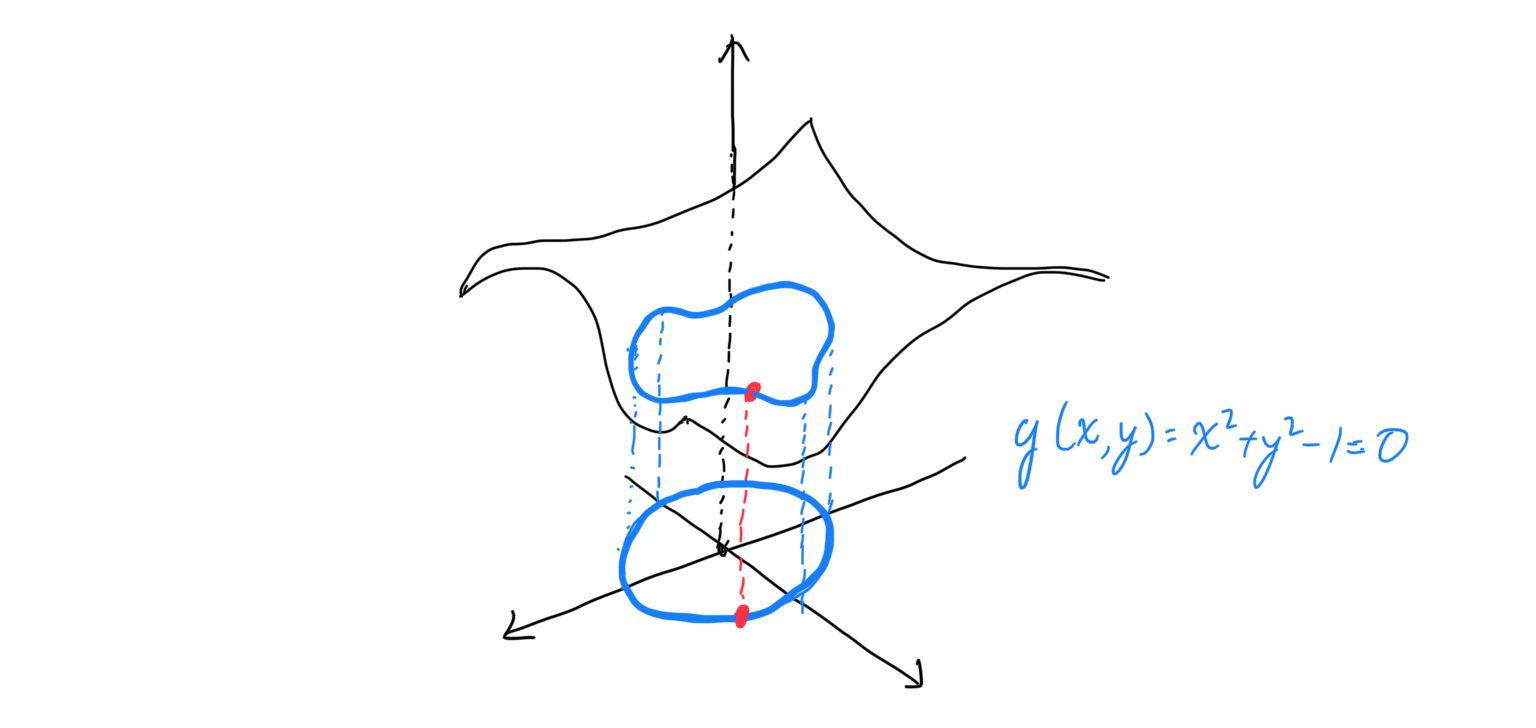
\includegraphics[scale=0.2]{img/Function_with_Constraints.PNG}
\end{center}
To solve this constraint problem, we use the method of Lagrange multipliers. The basic idea is to convert a constrained problem into a form such that the derivative test of an unconstrained problem can still be applied. The relationship between the gradient of the function and gradients of the constraints rather naturally leads to a reformulation of the original problem, known as the \textit{Lagrangian function}. That is, in order to find the maximum/minimum of $f$ subjected to the equality constraint $\mathbf{g}(\mathbf{x}) = \mathbf{0}$, we form the Lagrangian function
\[\mathcal{L}(\mathbf{x}, \lambda) \equiv f(\mathbf{x}) - \boldsymbol{\lambda}^T \mathbf{g}(\mathbf{x})\]
and find the stationary points of $\mathcal{L}$ considered as a function of $\mathbf{x} \in D$ and the Lagrange multiplier $\lambda \in \mathbb{R}$. The main advantage to this method is that it allows the optimization to be solved without explicit parameterization in terms of the constraints. 

\begin{theorem}[Lagrange Multipliers Theorem]
Let $f: \mathbb{R}^n \longrightarrow \mathbb{R}$ be a $C^1$ function and let $g(\mathbf{x}) = 0$, where $g: \mathbb{R}^n \longrightarrow \mathbb{R}^c$, be a system of $C^1$ constraint equations: $g \coloneqq (g_1, g_2, \ldots, g_c)$. Let $\mathbf{x}^*$ be an optimal solution to the optimization problem of maximizing $f(\mathbf{x})$ subject to the constraint $g(\mathbf{x}) = 0$ such that $\rank D g_{\mathbf{x}^*} = c < n$. Then, their exists a unique vector $\boldsymbol{\lambda}^*$ of Lagrange multipliers $\lambda_1^*, \lambda_2^*, \ldots, \lambda_c^*$ s.t. 
\[D f_{\mathbf{x}^*} = \lambda^{*T} D g_{\mathbf{x}^*}\]
where $D f_{\mathbf{x}^*}$ can be interpreted as the $1 \times n$ Jacobian matrix of $f$ and $D g_{\mathbf{x}^*}$ as the $c \times n$ Jacobian of $g$. Since both $D f_{\mathbf{x}^*}$ and $\lambda^{*T} D g_{\mathbf{x}^*}$ are maps from $\mathbb{R}^n$ to $\mathbb{R}$, we can invoke Riesz representation theorem to turn this into gradients: 
\[\nabla f(\mathbf{x}^*) = \nabla \mathbf{g}(\mathbf{x}^*) (\boldsymbol{\lambda}^*)\]
which has a matrix realization of 
\begin{align*}
\begin{pmatrix}
\frac{\partial f}{\partial x_1} (\mathbf{x}^*) \\ \vdots\\ \frac{\partial f}{\partial x_n} (\mathbf{x}^*) \end{pmatrix} & = \begin{pmatrix}
\frac{\partial g_1}{\partial x_1} (\mathbf{x}^*)& \ldots & \frac{\partial g_c}{\partial x_1} (\mathbf{x}^*)\\
\vdots & \ddots & \vdots \\
\frac{\partial g_1}{\partial x_n} (\mathbf{x}^*)& \ldots & \frac{\partial g_c}{\partial x_n}(\mathbf{x}^*)
\end{pmatrix} \begin{pmatrix}
\lambda^*_1 \\ \vdots \\ \lambda^*_c \end{pmatrix} \\
& = \lambda^*_1 \begin{pmatrix}
\frac{\partial g_1}{\partial x_1} (\mathbf{x}^*) \\ \vdots \\ \frac{\partial g_1}{\partial x_n}(\mathbf{x}^*)
\end{pmatrix} + \lambda^*_2 \begin{pmatrix}
\frac{\partial g_2}{\partial x_1} (\mathbf{x}^*) \\ \vdots \\ \frac{\partial g_2}{\partial x_n}(\mathbf{x}^*)
\end{pmatrix} + \ldots + \lambda^*_c \begin{pmatrix}
\frac{\partial g_c}{\partial x_1} (\mathbf{x}^*) \\ \vdots \\ \frac{\partial g_c}{\partial x_n}(\mathbf{x}^*)
\end{pmatrix}
\end{align*}
This equation tells us that at any critical points $\mathbf{x}^*$ of $f$ evaluated under the equality constraints, the gradient of $f$ at $\mathbf{x}^*$ can be expressed as a unique linear combination of the gradients of the constraints $\nabla g_i (\mathbf{x}^*)$ (at $\mathbf{x}^*$), with the Lagrange multipliers acting as coefficients. Therefore, finding the critical points $\mathbf{x}^*$ of $f$ constrained with $g$ is equivalent to solving the system of $c + n$ equations for the $n$ unknowns in $\mathbf{x}$ and $c$ unknowns in $\boldsymbol{\lambda}$: 
\begin{align*}
    \mathbf{g}(\mathbf{x}) & = 0 \\ 
    \nabla f(\mathbf{x}) & = \nabla \mathbf{g}(\mathbf{x}) (\boldsymbol{\lambda})
\end{align*} 
which can be rewritten as
\begin{align*}
    c \text{ constraint equations} & \begin{cases}
    g_1 (x) & = 0 \\
    \ldots & = 0 \\
    g_c (x) & = 0
    \end{cases} \\
    n \text{ Lagranaian equations} & \begin{cases}
   \frac{\partial f}{\partial x_1} (\mathbf{x}^*) & = \lambda^*_1 \frac{\partial g_1}{\partial x_1} (\mathbf{x}^*) + \lambda^*_2 \frac{\partial g_2}{\partial x_1} (\mathbf{x}^*) + \ldots + \lambda^*_c \frac{\partial g_c}{\partial x_1} (\mathbf{x}^*) \\
    \ldots & = \ldots \\
    \frac{\partial f}{\partial x_n} (\mathbf{x}^*) & = \lambda^*_1 \frac{\partial g_1}{\partial x_n} (\mathbf{x}^*) + \lambda^*_2 \frac{\partial g_2}{\partial x_n} (\mathbf{x}^*) + \ldots + \lambda^*_c \frac{\partial g_c}{\partial x_n} (\mathbf{x}^*) 
    \end{cases}
\end{align*}
\end{theorem}

More abstractly, $D f_{\mathbf{x}^*}$ is the linear functional in $(\mathbb{R}^n)^*$, and $D g_{\mathbf{x}^*}$, which is a linear map from $\mathbb{R}^n$ to $\mathbb{R}^c$, can be interpreted as a map from $(\mathbb{R}^c)^*$ to $(\mathbb{R}^n)^*$ Since $\boldsymbol{\lambda}^*$ "lives" in $(\mathbb{R}^c)^*$, $D g_{\mathbf{x}^*}(\boldsymbol{\lambda}^*) \in (\mathbb{R}^n)^*$, which is the same space that $f_{\mathbf{x}^*}$ lives in. 


Let us introduce a visualization for when where is a single constraint $g: \mathbb{R}^n \longrightarrow \mathbb{R}$. From the properties of the gradient, $\nabla f(x_0)$ is orthogonal to the level set of points satisfying $f(x) = f(x_0)$ at point $x_0$. Note that the constraint function $g$ also maps $\mathbb{R}^n \longrightarrow \mathbb{R}$, and so it has its own level surfaces. We can see that the point where the contour line of $g(x) = 0$ tangentially touches the contours of $f$ is the maximum. Since it intersects it tangentially, the gradient vector at that point $\nabla g(x_0)$ is parallel to $\nabla f(x_0)$. 
\begin{center}
    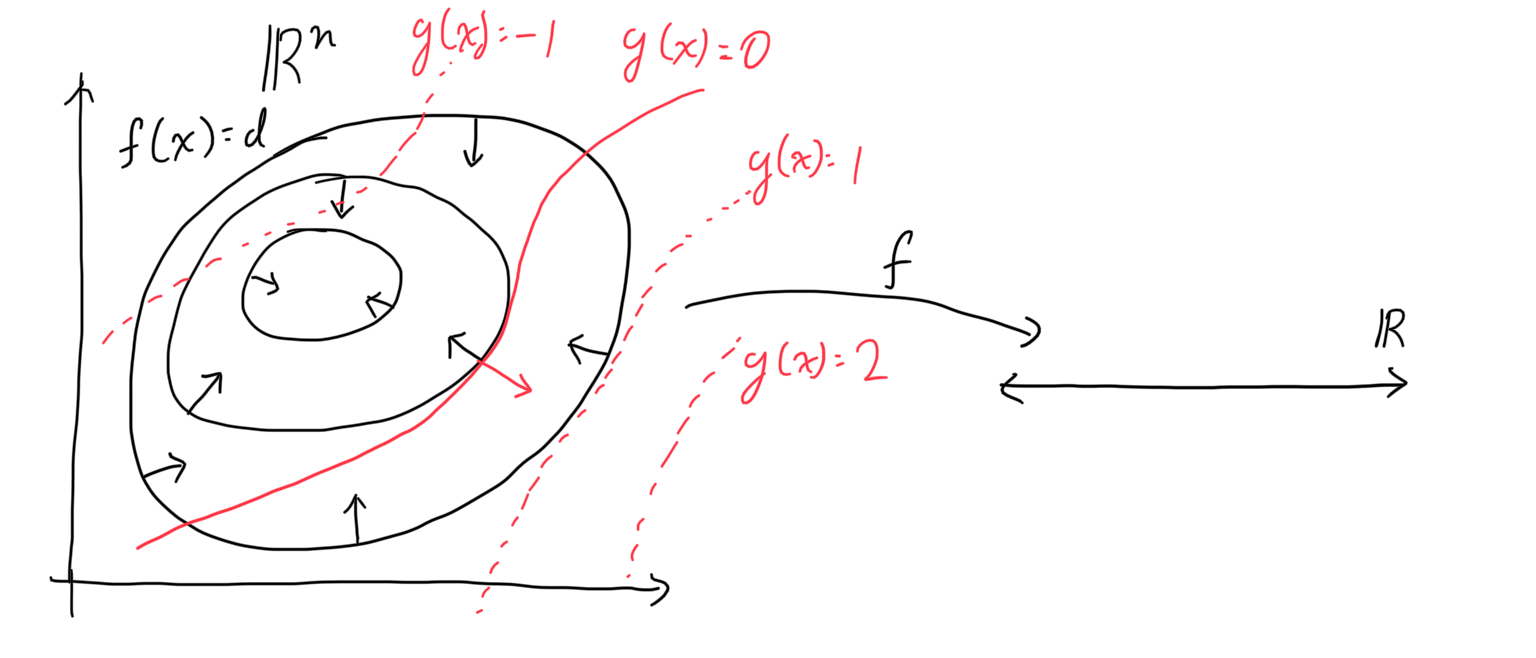
\includegraphics[scale=0.22]{img/Lagrange_Multiplier_Single_Constraint.PNG}
\end{center}
We can visualize this for multiple constraints as well, where $\nabla f(x_0)$ (the gradient vector of $f$ at $x^*$) can be expressed as a linear combination of $\nabla g_1 (x_0)$ and $\nabla g_2 (x_0)$ (gradient vectors of the constraint functions at $x^*$). 
\begin{center}
    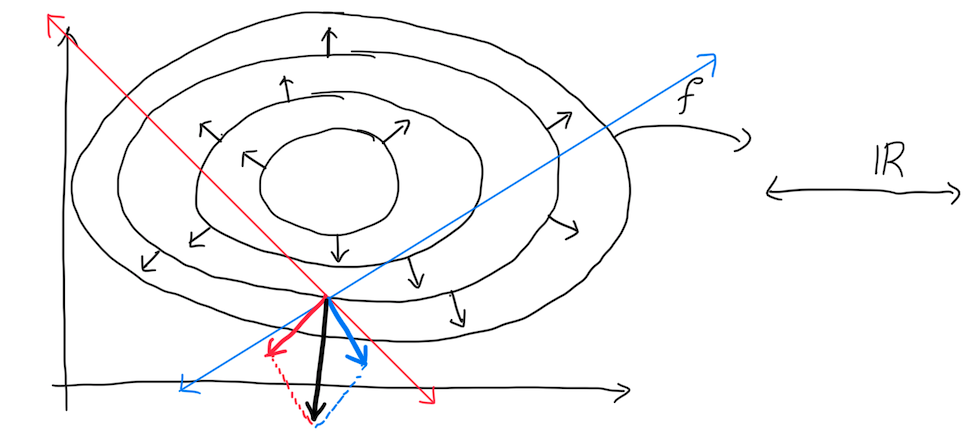
\includegraphics[scale=0.27]{img/Lagrange_Multiplier_Multiple_Constraints.PNG}
\end{center}

From the properties of the gradient introduced before, $\triangledown f(x_0)$ is orthogonal to the level set of points satisfying $f(x) = c$ at the point $x_0$. But this level set $f(x) = c$ actually intersects the level set determined by $g(x) = c$ at the point $x_0$ and is indistinguishable from each other at $x_0$. This means that $\triangledown g(x_0)$ is normal the level set of $g(x) = c$ at $x_0 \iff $ it is normal to the level set of $f(x) = c$ at $x_0$. But $\triangledown f(x_0)$ is also normal at that point, so $\triangledown f(x_0)$ must be parallel to $\triangledown g(x_0)$. 


\section{Implicit, Inverse Function Theorem}

\subsection{Inverse Function Theorem}
A special case of the general implicit function theorem is the inverse function theorem. It gives sufficient condition for a function to be invertible in a neighborhood of a point in its domain. 

\begin{theorem}[Inverse Function Theorem for Single-Variable $C^1$ Functions]
If $f: \mathbb{R} \longrightarrow \mathbb{R}$ is a $C^1$ function with a nonzero derivative at point $x_0$, then $f$ is invertible in a neighborhood of $x_0$, the inverse is also $C^1$, and the derivative of the inverse function at $y_0 = f(x_0)$ is the reciprocal of the derivative of $f$ at $x_0$. 
\[\big( f^{-1}\big)^\prime (y_0) = \frac{1}{f^\prime (x_0)}\]
This can be visualized easily by looking at the graph of any $C^1$ function. 
\begin{center}
    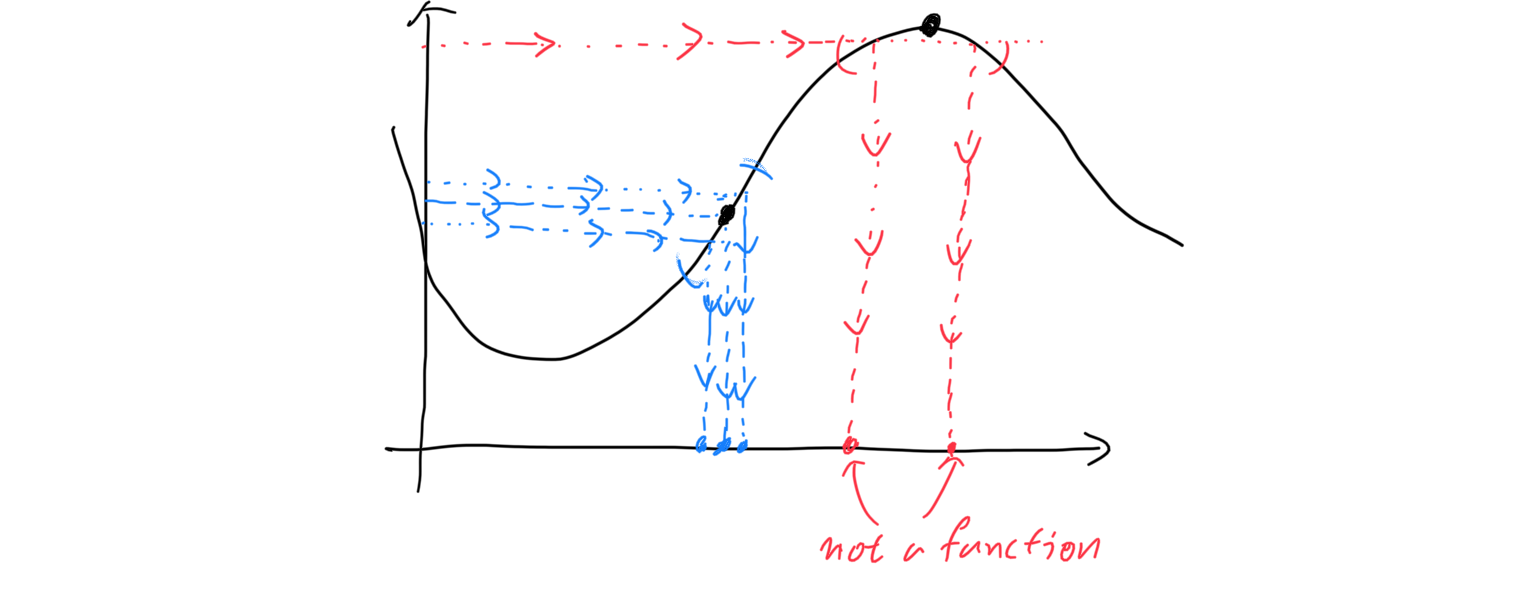
\includegraphics[scale=0.25]{img/Inverse_Function_Theorem_One_Variable.PNG}
\end{center}
In high school mathematics, this theorem is informally presented as the \textit{horizontal line test}. 
\end{theorem}

This can be stated in an alternative form: If $f: \mathbb{R} \longrightarrow \mathbb{R}$ is continuous and injective near $x_0$, and differentiable at $x_0$ such that $f^\prime (x_0) \neq 0$, then $f$ is invertible near $x_0$ with an inverse that's similarly continuous and injective, and where the above formula would apply as well. 

\begin{corollary}[Inverse Function Theorem for Single-Variable $C^k$ Functions]
If $f: \mathbb{R} \longrightarrow \mathbb{R}$ is a $C^k$ functions with a nonzero derivative at point $x_0$, then $f$ is invertible in a neighborhood of $x_0$, the inverse is also $C^k$, and the derivative of the inverse function at $y_0 = f(x_0)$ is the reciprocal of the derivative of $f$ at $x_0$. 
\end{corollary}

\begin{theorem}[Inverse Function Theorem for Multivariable Functions and its Matrix Realization]
Let $\mathbf{f}: \mathbb{R}^n \longrightarrow \mathbb{R}^n$ be a $C^1$ function defined on an open neighborhood of $\mathbf{x}_0$ in the domain. If the total derivative/Jacobian $D \mathbf{f}_{\mathbf{x}_0}$ at $\mathbf{x}_0$ is invertible, an inverse function of $\mathbf{f}$ is defined on some neighborhood of $\mathbf{y}_0 = \mathbf{f}(\mathbf{x}_0)$. Given that we are working with a fixed basis, $\mathbf{f}$ can be modeled by the set of $n$ equations 
\begin{align*}
    f_1 (x_1, x_2, \ldots, x_n) &= y_1 \\
    \ldots & = \ldots \\
    f_2 (x_1, x_2, \ldots, x_n) &= y_2
\end{align*}
This theorem says that this system of $n$ equations has a unique solution for $x_1, x_2, \ldots, x_n$ in terms of $y_1, \ldots, y_n$, provided that we restrict $\mathbf{x}$ and $\mathbf{y}$ to small enough neighborhoods of $\mathbf{x}_0$ and $\mathbf{y}_0$. This inverse function $\mathbf{f}^{-1}: \mathbb{R}^n \longrightarrow \mathbb{R}^n$ is also $C^1$, and its total derivative/Jacobian $D \mathbf{f}^{-1}_{\mathbf{y}_0}$ at $\mathbf{y}_0 = \mathbf{f}(\mathbf{x}_0)$ is the inverse linear map of $D \mathbf{f}_{\mathbf{y}_0}$. 
\[D \mathbf{f}^{-1}_{\mathbf{y}_0} = \big( D \mathbf{f}_{\mathbf{x}_0} \big)^{-1}\]
\end{theorem}

\begin{example}
Consider the vector-valued function $\mathbf{f}: \mathbb{R}^2 \longrightarrow \mathbb{R}^2$ defined by 
\[\mathbf{f}(x_1, x_2) = \begin{pmatrix}
e^{x_1}\cos (x_2) \\ e^{x_1} \sin(x_2)
\end{pmatrix}\]
The total derivative/Jacobian matrix is 
\[J \mathbf{f}(x_1, x_2) = \begin{pmatrix}
e^{x_1} \cos(x_2) & - e^{x_1} \sin(x_2) \\
e^{x_1} \sin(x_2) & e^{x_1} \cos(x_2)
\end{pmatrix} \implies \det J \mathbf{f}(x_1, x_2) = e^{2x_1} \cos^2 (x_2) + e^{2x_1} \sin^2 (x_2) = e^{2x_1}\]
Since the determinant $e^{2x_1}$ is nonzero everywhere, $D \mathbf{f}_\mathbf{x}$ is nonsingular. Thus, the theorem guarantees that for every point $\mathbf{x}_0 \in \mathbb{R}^2$, there exists a neighborhood about $\mathbf{x}_0$ over which $\mathbf{f}$ is invertible. However, this does not mean $\mathbf{f}$ is invertible over its entire domain: in this case $\mathbf{f}$ isn't even injective since it is periodic: e.g. the preimage of $(e, 0)$ contains $(1, 0)$ and $(1, 2\pi)$. 
\end{example}

\subsection{Implicit Function Theorem}
Remember that given an explicit representation of a set $\mathbf{y} = \mathbf{f}(\mathbf{x})$, we can easily find the implicit form as $\mathbf{F}(\mathbf{x}, \mathbf{y}) = \mathbf{y} - \mathbf{f}(\mathbf{x}) = \mathbf{0}$. What about the other way around? That is, given an implicit representation of some surface, what conditions must be met so that it can be represented as the graph of a function? The implicit function theorem is a tool that allows relations between points in $\mathbb{R}^n$ to be converted to functions of several real variables. That is, it states that for sufficiently "nice" points on a $n$-dimensional surface defined as $\mathbf{F}(\mathbf{x}, \mathbf{y}) = \mathbf{0}$ (where $\mathbf{F}: \mathbb{R}^{n+m} \longrightarrow \mathbb{R}^m$), we can locally pretend that this surface is a graph of a function $\mathbf{g}: \mathbb{R}^n \longrightarrow \mathbb{R}^m$ whose graph $\big(\mathbf{x}, \mathbf{g}(\mathbf{x})\big)$ is precisely the set of all $(\mathbf{x}, \mathbf{y})$ s.t. $\mathbf{f}(\mathbf{x}, \mathbf{y}) = \mathbf{0}$. When $m = 1$, it basically states that if an implicit surface suffices the vertical line test in a neighborhood, then it can be written as a function. 

\begin{example}[Circle]
Let $f: \mathbb{R}^2 \longrightarrow \mathbb{R}$ be defined by $f(x, y) = x^2 + y^2 - 1$. The level set at $z = 0$ would be the set of points satisfying 
\[x^2 + y^2 - 1 = 0\]
the unit circle. The derivative of $f$ with respect to $y$ is $0$ at the points $(-1,0)$ and $(1,0)$, meaning that in any neighborhood of these points, we cannot define a function of $y$ with respect to $x$. This is true, indeed, since any such function would fail the vertical line test, which can be seen in the red neighborhood around $(1,0)$. However, the blue neighborhood of the point $(-\sqrt{2}/2, \sqrt{2}/2)$ does indeed define a function of $y$ with respect to $x$ satisfying the vertical line test. 
\begin{center}
\begin{tikzpicture}
    \draw[<->] (-3,0)--(3,0);
    \draw[<->] (0,-3)--(0,3);
    \draw (0,0) circle (2);
    \draw[fill=red] (2,0) circle (0.08);
    \draw[fill=red] (-2,0) circle (0.08);
    \draw[red, thick] (1.732, -1) arc (-30:60:2);
    \draw[dashed, <->] (1.8,-2.5)--(1.8,2.5);
    \draw[fill=blue] (-1.414, 1.414) circle (0.08);
    \draw[blue, thick] (-1, 1.732) arc (120:170:2);
    \draw[dashed,<->] (-1.7,2.5)--(-1.7,-2.5);
\end{tikzpicture}
\end{center}
\end{example}

\begin{theorem}[Implicit Function Theorem in $\mathbb{R}^2$]
Let $f: \mathbb{R}^2 \longrightarrow \mathbb{R}$ be a $C^1$ function with a point $\mathbf{a} = (a_1, a_2)$ on the level set $f(\mathbf{x}) = 0$. If 
\[\partial_{x_2} f (\mathbf{a}) \neq 0\]
then there is an open neighborhood $U$ around $a_1$ such that we can make $x_2$ a function of $x_1$ within $U$ satisfying $f(x_1, x_2(x_1)) = 0$. That is, we can find a $x_2: \mathbb{R} \longrightarrow \mathbb{R}$ s.t. the graph of $x_2(x_1)$ within $U$ coincides with the graph of $f(\mathbf{x}) = 0$.
\end{theorem}

\begin{theorem}[Implicit Function Theorem in $\mathbb{R}^3$]
Let $f: \mathbb{R}^3 \longrightarrow \mathbb{R}$ be a $C^1$ function with a point $\mathbf{a} = (a_1, a_2, a_3)$ on the level set $f(\mathbf{x}) = 0$. If 
\[\partial_{x_3} f (\mathbf{a}) \neq 0\]
then there is an open neighborhood $U$ around $(a_1, a_2)$ such that we can make $x_3$ a function of $x_1$ and $x_2$ within $U$ satisfying $f(x_1, x_2, x_3(x_1 x_2)) = 0$. That is, we can find a $x_3: \mathbb{R}^2 \longrightarrow \mathbb{R}$ s.t. the graph of $x_3(x_1, x_2)$ within $U$ coincides with the graph of $f(\mathbf{x}) = 0$.
\end{theorem}

Note that for the 2D and 3D case, the level surface that we dealt with has a codimension of $1$. 

\begin{definition}[Truncated Jacobian Matrix]
Given a function $\mathbf{f}: \mathbb{R}^{n+m} \longrightarrow \mathbb{R}^m$ where the variables are 
\[x_1, \ldots, x_n, y_1, \ldots, y_m\]
the \textit{truncated Jacobian matrix} of $f$ can either refer to
\begin{enumerate}
    \item the $m \times n$ matrix formed by the leftmost $n$ columns of $D f$, which we will denote $D_\mathbf{x} f$, or 
    \item the $m \times m$ matrix formed by the rightmost $m$ columns of $D f$, which we will denote $D_\mathbf{y} f$. 
\end{enumerate}
\[D f = \begin{pmatrix} D_\mathbf{x} f & D_\mathbf{y} f \end{pmatrix} = \left(\begin{array}{ccc|ccc}
   \frac{\partial f_1}{\partial x_1} &\ldots &\frac{\partial f_1}{\partial x_n} & \frac{\partial f_1}{\partial y_1} & \ldots & \frac{\partial f_1}{\partial y_m}\\
   \vdots & \ddots & \vdots & \vdots & \ddots & \vdots \\
   \frac{\partial f_m}{\partial x_1} &\ldots &\frac{\partial f_m}{\partial x_n} & \frac{\partial f_m}{\partial y_1} & \ldots & \frac{\partial f_m}{\partial y_m}
   \end{array}\right)\]
\end{definition}

\begin{theorem}[Special Implicit Function Theorem]
Let $f: \mathbb{R}^{n+1} \longrightarrow \mathbb{R}$ be a $C^1$ function with a point $(\mathbf{a}, b) \in \mathbb{R}^{n+1}$ on the level set $f(\mathbf{x}, y) = 0$. If $\partial_y f (\mathbf{a}, b)$, which can also be thought of as the $1 \times 1$ truncated Jacobian matrix $D_\mathbf{y} f_{(\mathbf{a}, b)} = \partial_{y} f(\mathbf{a}, b)$ w.r.t. $y$, of 
\[D f_{(\mathbf{a}, b)} = \begin{pmatrix} D_\mathbf{x} f_{(\mathbf{a}, b)} & D_\mathbf{y} f_{(\mathbf{a}, b)} \end{pmatrix} = \left(\begin{array}{ccc|c}
   \partial_{x_1} f(\mathbf{a}, b) &\ldots & \partial_{x_n} f(\mathbf{a}, b) & \partial_{y} f(\mathbf{a}, b)
   \end{array}\right)\]
is invertible (in this case nonzero), then there exists an open neighborhood $U_\mathbf{a} \subset \mathbb{R}^n$ of $\mathbf{a}$ and a unique $C^1$ function $y: U \subset \mathbb{R}^n \longrightarrow \mathbb{R}$ s.t. $f\big(\mathbf{x}, y(\mathbf{x})\big) = 0$ for all $\mathbf{x} \in U$. That is, we can find a $y: U \longrightarrow \mathbb{R}$ s.t. the graph $y(\mathbf{x})$ within $U$ coincides with the graph of $f(\mathbf{x}, y) = 0$. Moreover, the total derivative/Jacobian of $y: \mathbb{R}^n \longrightarrow \mathbb{R}$ in $U$ is the $1 \times n$ matrix given by the matrix product
\[D g_\mathbf{a} = - (D_y f_\mathbf{a})^{-1} D_\mathbf{x} f_\mathbf{a}\]
\end{theorem}

\begin{example}[Circle Example]
Let $n = m = 1$ and $f(x_1, x_2) = x_1^2 + x_2^2 - 1$. We would like to find out at which points $\mathbf{a}$ can this surface be explicitly represented by a function $g: U_\mathbf{a} \subset \mathbb{R} \longrightarrow \mathbb{R}$ defining $x_2$ from $x_1$. Its Jacobian is 
\[D f = \begin{pmatrix} \partial_{x_1} f & \partial_{x_2} f \end{pmatrix} = \begin{pmatrix} 2 x_1 & 2x_2 \end{pmatrix} \]
The truncated Jacobian w.r.t. $x_2$ is $2 x_2$, which is invertible iff $x_2 \neq 0$. By the implicit function theorem, we can locally write the circle in the form $x_2 = g(x_1)$ for all points where $x_2 \neq 0$. This is easy to see. For example, we can choose the point $(0.8, 0.6)$ on the level set, and the appropriate explicit function is 
\[x_2 = g(x_1) = \sqrt{1 - x_1^2}\]
within the neighborhood of $x_1 = 0.8$. For $(\pm 1, 0)$, we cannot since every function defined within a neighborhood of $x_1 = \pm 1$ fails the vertical line test. The derivative of $g$, by the theorem, can be defined implicitly as 
\[D g = - ( \partial_{x_2} f)^{-1} D_{x_1} f = - (2 x_2)^{-1} (2 x_1) = -\frac{x_1}{x_2}\]
which leads to the differential equation 
\[g^\prime (x_1) = - \frac{x_1}{g(x_1)} \text{ where we solve for } g\]
If we would have liked to find a function $h: U_{a_{\mathbf{x}_2}} \subset \mathbb{R} \longrightarrow \mathbb{R}$ defining $x_1$ from $x_2$, then we can redo everything to find that the truncated Jacobian w.r.t. $x_1$ is $2x_1$, which is invertible iff $x_1 \neq 0$, and the the derivative is 
\[D h = - (\partial_{x_1} f)^{-1} D_{x_2} f = - (2x_1)^{-1} (2x_2) = -\frac{x_2}{x_1}\]
which leads to the differential equation 
\[h^\prime (x_2) = - \frac{x_2}{h(x_2)} \text{ where we solve for } h\]
\end{example}

\begin{theorem}[General Implicit Function Theorem]
Let $f: \mathbb{R}^{n+m} \longrightarrow \mathbb{R}^m$ be a $C^1$ function with a point $(\mathbf{a}, \mathbf{b}) \in \mathbb{R}^{n + m}$ on the level set $f( \mathbf{x}, \mathbf{y}) = 0$. If the $m \times m$ truncated Jacobian matrix $D_{\mathbf{y}} f (\mathbf{a}, \mathbf{b})$ w.r.t. $\mathbf{y}$, of 
\[D f_{(\mathbf{a}, \mathbf{b})} = \begin{pmatrix} D_\mathbf{x} f_{(\mathbf{a}, \mathbf{b})} & D_\mathbf{y} f_{(\mathbf{a}, \mathbf{b})} \end{pmatrix}\]
is invertible, then there exists an open neighborhood $U_\mathbf{a} \subset \mathbb{R}^n$ of $\mathbf{a}$ and a unique $C^1$ function $\mathbf{y}: U \subset \mathbb{R}^n \longrightarrow \mathbb{R}^m$ s.t. $f\big(\mathbf{x}, \mathbf{y}(\mathbf{x}) \big) = 0$ for all $\mathbf{x} \in U$. That is, we can find a $\mathbf{y}: U \longrightarrow \mathbb{R}^m$ s.t. the graph $\mathbf{y}(\mathbf{x})$ within $U$ coincides with the graph of $f(\mathbf{x}, \mathbf{y}) = 0$. Moreover, the total derivative/Jacobian of $\mathbf{y}$ is the $m \times n$ matrix given by the matrix product 
\[D g_\mathbf{a} = - (D_\mathbf{y} f_\mathbf{a})^{-1} D_\mathbf{x} f_\mathbf{a}\]
\end{theorem}

\section{Change of Basis} 

\section{Divergence and Curl}

\subsection{Divergence}

Colloquially, the divergence is an operator $\Div$ that operates on a vector field and produces a scalar field which provides the quantity of the vector field's source at each point. Technically, the divergence represents the volume density of the outward flux of a vector field from an infinitesimal volume around a given point. 

There is a very nice geometric interpretation for divergence. Imagine that the vector field $F$ represents fluid flow in $\mathbb{R}^n$. Divergence is then the "measure" of the net amount of fluid flowing in and out of an infinitesimally small region, labeled at each point. If the net fluid flow is positive (i.e. more fluid is flowing in than out) at point $x_0$, then $\Div{F}(x_0) > 0$. If the net fluid flow is negative (i.e. more fluid is flowing out than in) at point $x_0$, then $\Div{F}(x_0) < 0$. This measure assigns a number to every point in the space (creating a scalar field). Therefore, each point either acts as a "source" of fluid emanating from it or as a "sink" that sucks in more fluid than it puts out. 
\begin{center}
    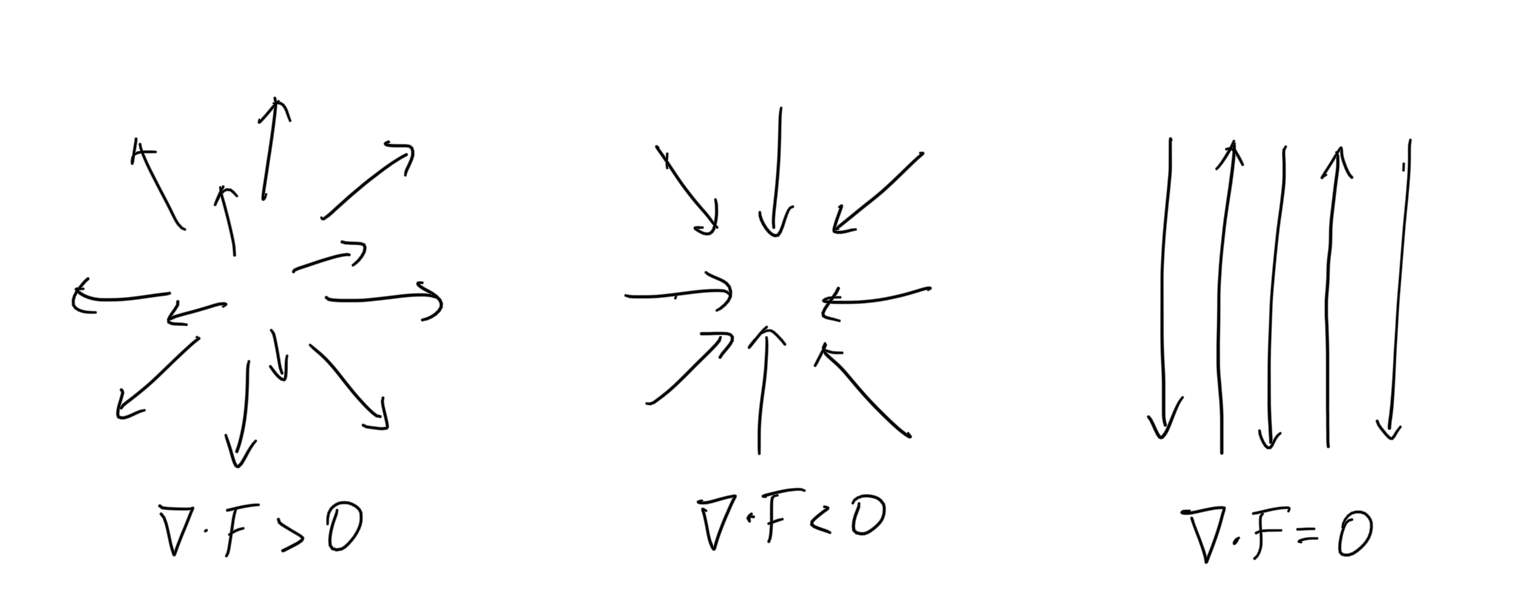
\includegraphics[scale=0.25]{img/Divergence_compared_to_Zero.PNG}
\end{center}

\begin{definition}[Divergence]
The \textbf{divergence} of a vector field $\mathbf{F}: \mathbb{R}^n \longrightarrow \mathbb{R}^n$ is a scalar field defined 
\[\Div \mathbf{F} \coloneqq \nabla \cdot \mathbf{F} = \begin{pmatrix} \frac{\partial}{\partial x_1} \\ \vdots \\ \frac{\partial}{\partial x_n} \end{pmatrix} \cdot \begin{pmatrix} F_1 \\ \vdots \\ F_n \end{pmatrix} = \sum_i \frac{\partial \mathbf{F}_i}{\partial x_i}\]
When $n = 1$, $\mathbf{F}$ reduces to a regular function and $\Div \mathbf{F} $ reduces to the ordinary derivative. Some further properties: 
\begin{enumerate}
    \item By linearity of partials, $\Div$ is also a linear operator. That is, given two vector fields $\mathbf{F}, \mathbf{G}$ and two scalars $\alpha, \beta$, 
    \[\Div (\alpha \mathbf{F} + \beta \mathbf{G}) = \alpha \Div \mathbf{F} + \beta \Div \mathbf{G}\]
    
    \item Divergence satisfies the product rule: Given a vector field $\mathbf{F}: \mathbb{R}^n \longrightarrow \mathbb{R}^n$ and a scalar function $\varphi: \mathbb{R}^n \longrightarrow \mathbb{R}$. 
    \[\nabla \cdot (\varphi \mathbf{F}) = \nabla \varphi \cdot \mathbf{F} + \varphi (\nabla \cdot \mathbf{F})\]
\end{enumerate}
\end{definition}

\begin{example}
The divergence of the origin in the left graph is clearly negative since the net flow is out of the point, while the divergence of the origin in the right graph is positive since the net fluid flow is in. 
\begin{center}
\pgfplotsset{width=7cm,compat=1.16}
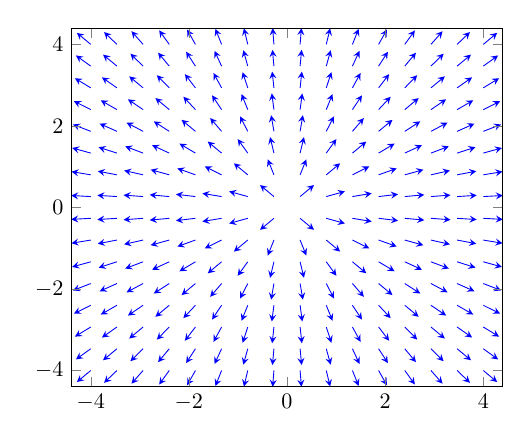
\begin{tikzpicture}[scale=0.8]
\begin{axis}[view={0}{90}, domain=-4:4]
\addplot3 [blue,-stealth,samples=16,
        quiver={
            u={2*x/pow(x^2 + y^2,1/2)},
            v={2*y/pow(x^2 + y^2,1/2)},
            scale arrows=0.2,
        },
    ] { 1};
\end{axis}
\end{tikzpicture}
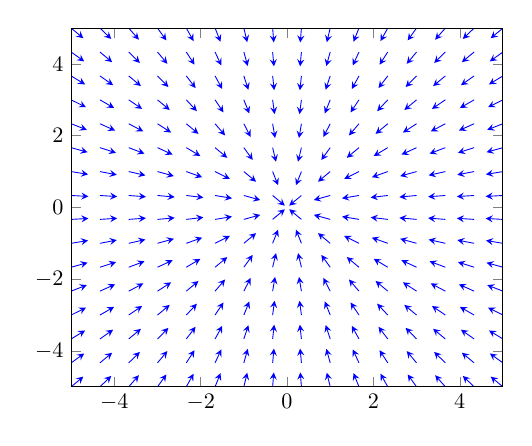
\begin{tikzpicture}[scale=0.8]
\begin{axis}[view={0}{90}]
\addplot3 [blue,-stealth,samples=16,
        quiver={
            u={-2*x/pow(x^2 + y^2,1/2)},
            v={-2*y/pow(x^2 + y^2,1/2)},
            scale arrows=0.2,
        },
    ] { 1};
\end{axis}
\end{tikzpicture}
\end{center}
\end{example}

\begin{lemma}[Divergence in Cylindrical Coordinates]
For vector field $F: \mathbb{R}^3 \longrightarrow \mathbb{R}^3$ expressed in cylindrical coordinates as 
\[F = \begin{pmatrix}
F_r \\ F_\theta \\ F_z
\end{pmatrix}\]
the divergence is
\[\Div F = \nabla \cdot F = \frac{1}{r} \frac{\partial}{\partial r} \big(r F_r \big) + \frac{1}{r} \frac{\partial F_\theta}{\partial \theta} + \frac{\partial F_z}{\partial z}\]
Note that the condition of locality is important, since in general a global cylindrical coordinate system would be inconsistent. 
\end{lemma}

\begin{lemma}[Divergence in Spherical Coordinates]
For vector field $F: \mathbb{R}^3 \longrightarrow \mathbb{R}^3$ expressed in spherical coordinates $(r, \theta, \phi)$, the divergence is 
\[\Div F = \nabla \cdot F = \frac{1}{r^2} \frac{\partial}{\partial r} \big( r^2 F_r) + \frac{1}{r \, \sin{\theta}} \frac{\partial}{\partial \theta} \big( \sin{\theta} F_\theta\big) + \frac{1}{r\, \sin{\theta}} \frac{\partial F_\phi}{\partial \phi}\]
\end{lemma}

\subsection{Curl}
Colloquially, the curl is a vector operator that describes the infinitesimal circulation of a vector field in $3$-dimensional Euclidean space, where the curl at each point is represented by a vector whose length and direction denote the magnitude and axis as the maximum circulation. That is, if one drops a twig or a ball with its center of mass at a certain point, the curl measures how much it will spin. In physics, the rotation of a rigid body in 3-dimensions can be described by a vector $\omega$ along the axis of rotation. $\omega$ is called the \textit{angular velocity vector}, with $||\omega||$ denoting the angular speed of the body. The curl of this vector field measured at the center of mass of the body is measured as $2 \omega$. That is, the curl outputs \textit{twice} the angular velocity vector of any rigid body. Note that unlike the gradient and divergence operators, curl does not generalize as simply to other dimensions. 

\begin{definition}[Curl]
The \textit{curl} of a 3-dimensional $C^k$ vector field $F: \mathbb{R}^3 \longrightarrow \mathbb{R}^3$ is an operator
\[\curl: C^k (\mathbb{R}^3; \mathbb{R}^3) \longrightarrow C^{k-1} (\mathbb{R}^3; \mathbb{R}^3)\]
defined
\[\curl{F} \equiv \nabla \times F \equiv \begin{pmatrix}
\frac{\partial}{\partial x} \\ \frac{\partial}{\partial y}\\ \frac{\partial}{\partial z} \end{pmatrix} \equiv \begin{pmatrix}
\frac{\partial F_3}{\partial y} - \frac{\partial F_2}{\partial z} \\
\frac{\partial F_1}{\partial z} - \frac{\partial F_3}{\partial x} \\
\frac{\partial F_2}{\partial x} - \frac{\partial F_1}{\partial y}
\end{pmatrix}\]
\end{definition}

\begin{definition}[Irrotational Vector Fields]
A vector field $F$ is \textit{irrotational} if 
\[\curl{F} = \mathbf{0}\]
Visually, this indicates that there are no "whirlpools" everywhere, meaning that any rigid body placed anywhere, while it may travel along a path, will not rotate around its own axis. 
\end{definition}

It has been shown that fluid draining from a tub is usually irrotational except for right at the center, which is surprising since the fluid itself is "rotating" around the drain. 

\begin{theorem}
For any $C^2$ vector field $F$, 
\[\Div{\curl{F}} = \nabla\cdot (\nabla \times F) = 0\]
That is, the divergence of any curl is 0. 
\end{theorem}
\begin{proof}
Proved by equality of mixed partials. 
\end{proof}

\begin{definition}
The \textit{Laplace operator}, or \textit{Laplacian}, of a function $f: \mathbb{R}^n \longrightarrow \mathbb{R}$ is the divergence of the gradient. 
\[\nabla^2 f \equiv \nabla \cdot (\nabla f) \equiv \sum_{i=1}^n \frac{\partial^2 f}{\partial x_i^2}\]
\end{definition}

\subsubsection{Conservative, Solenoidal Vector Fields}
\begin{definition}[Conservative Vector Fields]
A vector field $F: U \subset \mathbb{R}^n \longrightarrow \mathbb{R}^n$ is a \textit{conservative vector field} if and only if there exists a scalar field $f: U \subset \mathbb{R}^n \longrightarrow \mathbb{R}$ such that 
\[F = \nabla f\]
on $U$. 
\end{definition}

Conservative vector fields appear naturally in mechanics: they are vector fields representing forces of physical systems in which energy is conserved. 

\begin{theorem}
Given a $C^2$-function $f: \mathbb{R}^3 \longrightarrow \mathbb{R}$,
\[\nabla \times ( \nabla f) = 0\]
That is, the curl of any gradient vector field is the zero vector. 
\end{theorem}
\begin{proof}
$\nabla \times \nabla f$ can be expanded to
\[\bigg( \frac{\partial^2 f}{\partial y \partial z} - \frac{\partial^2 f}{\partial z \partial y}, \; \frac{\partial^2 f}{\partial z \partial x} - \frac{\partial^2 f}{\partial x \partial z}, \; \frac{\partial^2 f}{\partial x \partial y} - \frac{\partial^2 f}{\partial y \partial x}\bigg) = (0, 0, 0)\]
by equality of mixed partials. 
\end{proof}

\begin{definition}[Solenoidal Vector Fields]
A \textit{solenoidal, or incompressible, vector field} is a vector field $F: \mathbb{R}^n \longrightarrow \mathbb{R}^n$ such that
\[\Div F = \nabla \cdot F = 0\]
at all point in the field. That is, the field has no sources or sinks. 
\end{definition}

\begin{example}
The vector field $F: (x, y) \mapsto (y, -x)$ is solenoidal. 
\begin{center}
    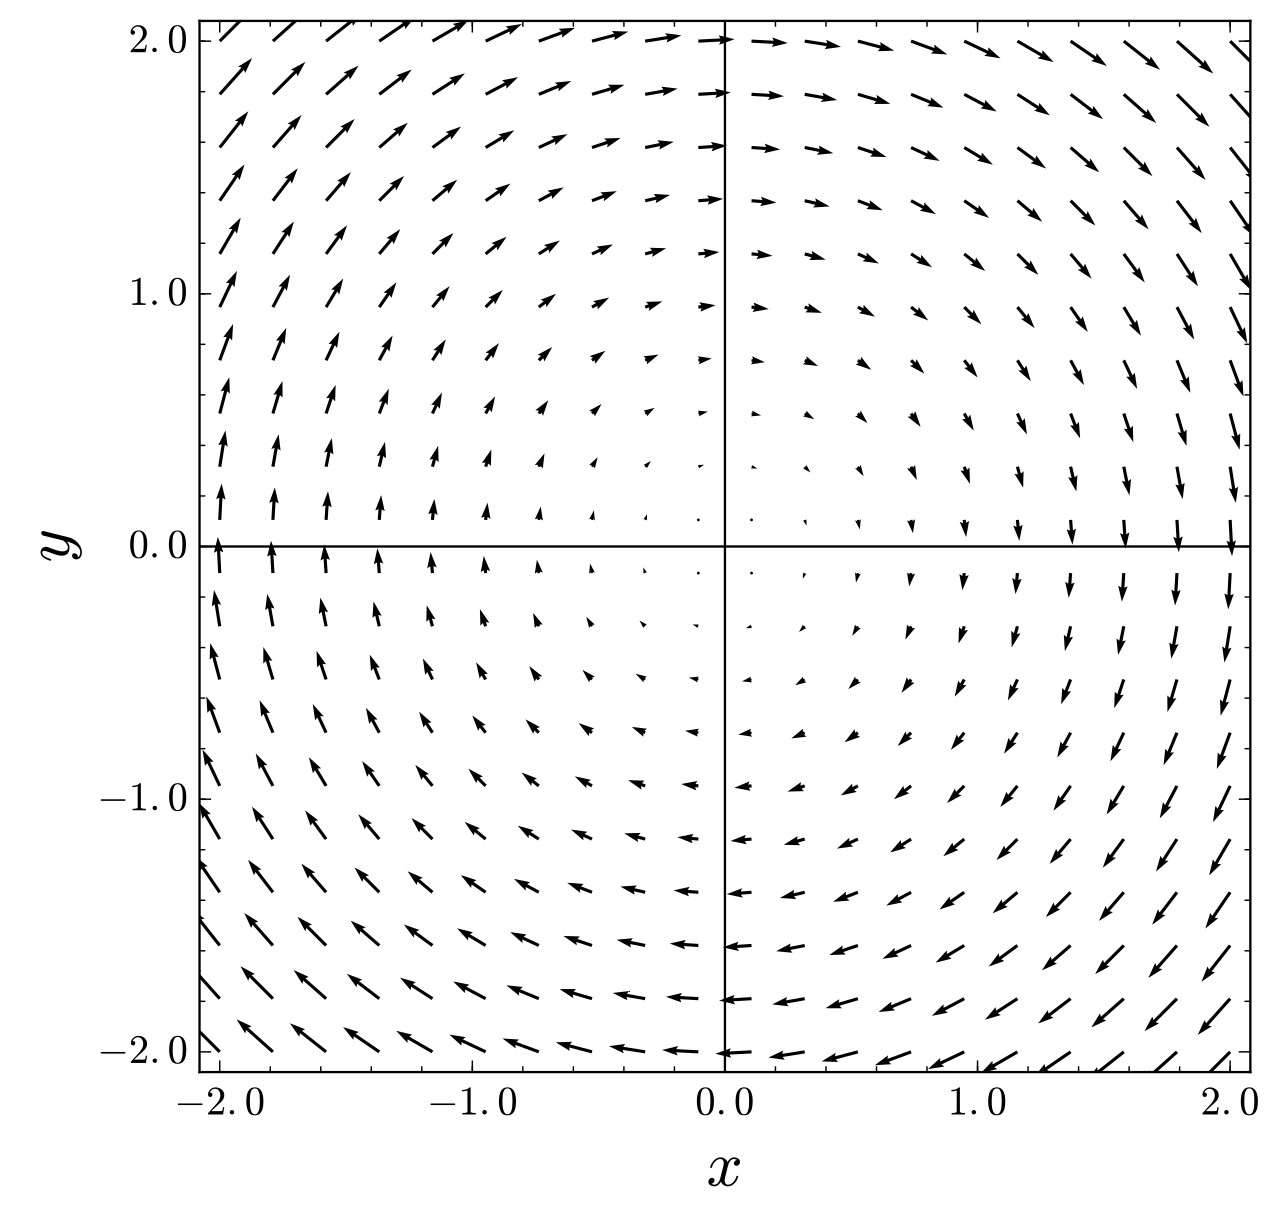
\includegraphics[scale=0.17]{img/Solenoidal_vector_field.png}
\end{center}
\end{example}

\section{Matrix Calculus}
Now we will take a look at functions that have either an input or output as matrices. Essentially, matrices are also vectors, so there is nothing new here to learn, but having a concrete set of notation is useful. First, note that when we talk about a total derivative $D \mathbf{f}_\mathbf{a}$, we can interpret this as a linear map that takes in some small perturbation $\mathbf{h}$ and gives us the result $D \mathbf{f}_\mathbf{a} (\mathbf{h})$. In our column-vector setting, this just corresponded to left matrix multiplication: 
\[D \mathbf{f}_\mathbf{a} (\mathbf{h}) = D \mathbf{f}_\mathbf{a} \mathbf{h}\]
This is not the case in the matrix setting. Let us compare the following: 
\begin{enumerate}
    \item The derivative of $f: \mathbb{R} \rightarrow \mathbb{R}$ at $a$ is a linear function $D f_a: \mathbb{R} \longrightarrow \mathbb{R}$ satisfying $f(a + h) \approx f(a) + D f_a (h) + O(h^2)$. But linearity reduces $D f_a$ to simply a scalar, and so our condition reduces to 
    
    \[f(a + h) \approx f(a) + D f_a h + O(h^2)\]
    
    \item The derivative of a path function $\mathbf{f}: \mathbb{R} \rightarrow \mathbb{R}^m$ is a linear function $D \mathbf{f}_a : \mathbb{R} \longrightarrow \mathbb{R}^m$ satisfying $\mathbf{f}(a + h) = \mathbf{f}(a) + D \mathbf{f}_a (h) + O(h^2)$. Linearity implies that $D \mathbf{f}_a$ is a rank-1 linear map, which reduces to it being a column vector, and our condition reduces to 
    \[\underbrace{\mathbf{f}(a + h)}_{m \times 1} \approx \underbrace{\mathbf{f}(a)}_{m \times 1} + \underbrace{D \mathbf{f}_a}_{m \times 1} \underbrace{h}_{1 \times 1}\]
    
    \item The derivative of a matrix function $\mathbf{F}: \mathbb{R} \rightarrow \mathbb{R}^{m \times n}$ is a linear map $D \mathbf{F}_a: \mathbb{R} \longrightarrow \mathbb{R}^{m \times n}$ satisfying $\mathbf{F}(a + h) \approx \mathbf{F}(a) + D \mathbf{F}_a (h)$. This time, linearity does not reduce it to simple left-hand matrix multiplication. We could just say that this is a left-hand scalar multiplication, but this doesn't generalize well, so we are stuck with just saying that $D \mathbf{F}_a$ is a linear map. 
    \[\underbrace{\mathbf{F}(a + h)}_{m \times n} \approx \underbrace{\mathbf{F}(a)}_{m \times n} + \underbrace{D \mathbf{F}_a (h)}_{m \times n}\]
\end{enumerate}
Now let us take a look at when we have matrix inputs. 
\begin{enumerate}
    \item The derivative of $f: \mathbb{R}^{m \times n} \longrightarrow \mathbb{R}$ is a linear function $D f_{\mathbf{A}} : \mathbb{R}^{m \times n} \longrightarrow \mathbb{R}$ satisfying $f(\mathbf{A} + \mathbf{H}) \approx f(\mathbf{A}) + D f_{\mathbf{A}} (\mathbf{H})$. We could let $D f_{\mathbf{A}}$ be some linear map like $\mathbf{M} \mapsto \mathbf{v}^T \mathbf{M} \mathbf{u}$, where $\mathbf{v}, \mathbf{u}$ is fixed. But in generality, we just have the condition 
    \[\underbrace{f(\mathbf{A} + \mathbf{H})}_{1 \times 1} \approx \underbrace{f(\mathbf{A})}_{1 \times 1} + \underbrace{D f_{\mathbf{A}} (\mathbf{H})}_{1 \times 1}\]
    
    \item The derivative of $\mathbf{f}: \mathbf{R}^{m \times n} \longrightarrow \mathbb{R}^d$ is some linear map $D \mathbf{f}_\mathbf{A} : \mathbf{R}^{m \times n} \longrightarrow \mathbb{R}^d$ satisfying $\mathbf{f} (\mathbf{A} + \mathbf{H}) \approx \mathbf{f}(\mathbf{A}) + D \mathbf{f}_\mathbf{A} (\mathbf{H})$. Again, we could construct some form that would give us a linear map in terms of some matrix multiplication, but in generality, we have the condition 
    \[\underbrace{\mathbf{f} (\mathbf{A} + \mathbf{H})}_{d \times 1} \approx \underbrace{\mathbf{f}(\mathbf{A})}_{d \times 1} + \underbrace{D \mathbf{f}_\mathbf{A} (\mathbf{H})}_{d \times 1}\]
\end{enumerate}

\subsection{Simple Differentiation Rules}

Now we present some theorems on basic differentiation. Proving these just requires us to expand the function and compute the derivatives component-wise. 

\begin{theorem}[Derivative of Affine Map]
Given $f: \mathbb{R}^n \longrightarrow \mathbb{R}^m$ defined $f(\mathbf{x}) = \mathbf{A} \mathbf{x} + \mathbf{b}$ (where $\mathbf{A}, \mathbf{b}$ is not dependent on $\mathbf{x}$), its derivative is 
\[D \mathbf{f} = \mathbf{A}\]
\end{theorem}

\begin{theorem}
Given the scalar $\alpha$ defined by 
\[\alpha = \mathbf{y}^T \mathbf{A} \mathbf{x}\]
where $\mathbf{y} \in \mathbb{R}^{m \times 1}, \mathbf{A} \in \mathbb{R}^{m \times n}$, and $\mathbf{x} \in \mathbb{R}^{n \times 1}$, then 
\[\frac{\partial \alpha}{\partial \mathbf{x}} = \mathbf{y}^T \mathbf{A} : \mathbb{R}^n \longrightarrow \mathbb{R}\]
and 
\[\frac{\partial \alpha}{\partial \mathbf{y}} = \mathbf{x}^T \mathbf{A}^T : \mathbb{R}^m \longrightarrow \mathbb{R}\]
Rewritten in the total derivative notation, we can interpret $\alpha$ as a function of both $\mathbf{x}$ and $\mathbf{y}$ and write 
\[D \alpha_{(\mathbf{x}, \mathbf{y})} = \begin{pmatrix} \mathbf{y}^T \mathbf{A} \\ \mathbf{x}^T \mathbf{A}^T \end{pmatrix} : \mathbb{R}^{n + m} \longrightarrow \mathbb{R}\]
\end{theorem}

\begin{theorem}
Given the scalar $\alpha$ defined by the quadratic form 
\[\alpha = \mathbf{x}^T \mathbf{A} \mathbf{x}\]
where $\mathbf{x} \in \mathbb{R}^{n \times 1}$ and $\mathbf{A} \in \mathbb{R}^{n \times n}$, then 
\[\frac{\partial \alpha}{\partial \mathbf{x}} = \mathbf{x}^T \big( \mathbf{A} + \mathbf{A}^T \big)\]
or in the total derivative notation, 
\[D \alpha_\mathbf{a} = \mathbf{a}^T \big( \mathbf{A} + \mathbf{A}^T \big) : \mathbb{R}^n \longrightarrow \mathbb{R}\]
\end{theorem}

\section{Integration}

\subsection{Geometric Interpretations of Integration}
The concept of integration in one variable calculus limits the applicability of the operation to finding only areas of functions under curves. We will replace the reader's intuition of integration with the following description. Given a function $f: \mathbb{R}^n \longrightarrow \mathbb{R}$, we interpret it as a scalar field that assigns a "weight" to each point in $\mathbb{R}^n$. Now, given any "shape" $B$ in $\mathbb{R}^n$ that is closed (but not necessarily bounded), an integral can calculate the "weighed" volume of $B$ by cutting $B$ into infinitesimally small points, multiplying them by their respective weights determined by $f$, and then summing up the weighed points. Integrating $B$ in $\mathbb{R}$, $\mathbb{R}^2$, and $\mathbb{R}^3$ with a constant scalar field equal to $1$ is equivalent to finding the length, area, and volume of $B$, respectively. We deconstruct specific types of iterated integrals. 

\subsubsection{Single Integral as Weighed Length or Area}
A single integral is calculated from a function $f: \mathbb{R} \longrightarrow \mathbb{R}$. Given some intervals (or a collection of intervals) $B \subset \mathbb{R}$, the integration notation is familiar to us. 
\[\int_B f(x) \; d x\]
We can interpret this integration in two ways. First, we imagine that the function $f$ is a scalar field in $\mathbb{R}$. Therefore, every point $x$ in $\mathbb{R}$ has a certain real number $f(x)$ associated to it. Therefore, the interval $B \in \mathbb{R}$ now consists of points that now have different densities each (which can be negative). The entire $B$ can now be thought of as a 1-dimensional "rod" in $\mathbb{R}$ that has an uneven distribution of mass determined by $f$. The total mass of the rod $B$ is calculated by the integral. In the diagram below, we use different "thickness" to represent different densities. 
\begin{center}
    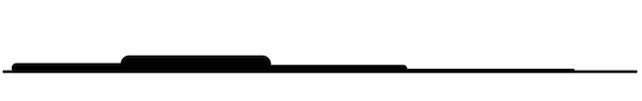
\includegraphics[scale=0.3]{img/Integral_As_Stick_with_Density.PNG}
\end{center}
Secondly, we can visualize the entire graph of $f$ in $\mathbb{R} \oplus \mathbb{R}$. This represents a curve in the $x y$-axis that most beginner calculus students are familiar with. Note that the interval $B$ exists in the x-axis, and in this case, the "weight" of each point $x$ in $B$ is represented as the "height" of the infinitesimally thin bar at $x$. It is easy to see that the weight of the rod at point $x$ and the height of the bar at point $x$ are really the same measure determined by $f$. Therefore, the density distribution in the rod is now modeled as the height of the function at each point. Calculating the integral of this function now calculates the "area" under the curve.

It is important to point out that $B$ does not necessarily need to be a length in the form of $[a,b]$. It can be any union of disjoint lengths, too. However, adding a finite number of single points to $B$ will not affect the integral. It is also customary for $B$ to be closed. 

\subsubsection{Double Integral as Weighed Area or Volume}
The double integral is calculated from function $f: \mathbb{R}^2 \longrightarrow \mathbb{R}$. Given a certain closed subset $B \subset \mathbb{R}^2$, the integration notation is
\[\iint_B f(x, y) \; d A\]

Again, we can interpret double integration in two ways. First, we think of $f$ as a scalar field assigning a density to every point in $\mathbb{R}^2$. Then, the 2-dimensional shape $B$ itself should have a certain density distribution on it determined by $f$. The double integral above then determines the mass of $B$. 

The second way to interpret this is to imagine the 2-dimensional shape $B$ lying in the extended space $\mathbb{R}^2 \oplus \mathbb{R}$. We then model the density distribution as merely the height of the infinitesimally thin bar at each point $x$. Again, the height of this bar at $x$ is precisely its density described in the first interpretation. Therefore, integrating this shape is equivalent to finding the volume of the infinite union of the infinitesimally thin bars at each point in $B$. 

Note again that $B$ need not be one solid region. It can be a union of multiple disjoint ones. However, adding a single point $p$ or a 1-dimensional path $p$ to $B$ will not affect the integral since they have an area of $0$.

\subsubsection{Triple Integral as Weighed Volumes or Hyper-Volumes}
The double integral is calculated from function $f: \mathbb{R}^3 \longrightarrow \mathbb{R}$. Given a certain closed subset $B \subset \mathbb{R}^3$, the integration notation is
\[\iiint_B f(x, y, z) \; d V\]
Following the logic of the previous two examples, the function $f$, interpreted as a scalar field, assigns a scalar at each point $x$ in the solid $B$. Therefore, we can visualize $B$ as a solid, 3-dimensional object in $\mathbb{R}^3$ with a certain density distribution defined by $f$. The total mass of $B$ is therefore determined by the triple integral above.

Following similar logic, we can interpret this integral as the hypervolume of a 4 dimensional object, but this is not often used. 

\subsection{Reduction to Iterated Integrals}
We first state a basic condition of integration. 

\begin{theorem}
Any function $f: \mathbb{R}^n \longrightarrow \mathbb{R}$ that is continuous over a certain region $B \subset \mathbb{R}^n$ can be integrated over $B$. 
\end{theorem}
That is, if $f$ is discontinuous at a certain subset $D \subset B$, then the infinitesimal neighborhoods around each point $d \in D$ is not well defined, since they would always contain two values of $f$ that do not converge to each other at $d$. 

However, there are some discontinuous functions that are in fact integrable. Assuming $B \subset \mathbb{R}^n$ is the region that we are integrating over, 
\begin{enumerate}
    \item Given that there is a subset $N$ in $B$ with volume $0$ over which $f$ is not defined, we can integrate over $B \setminus N$. In the one and two dimensional cases, 
    \[\int_{B \setminus N} f(x) dx \text{ and } \iint_{B\setminus N} f(x) dA\]
    are well-defined. Visually, 
    \begin{center}
        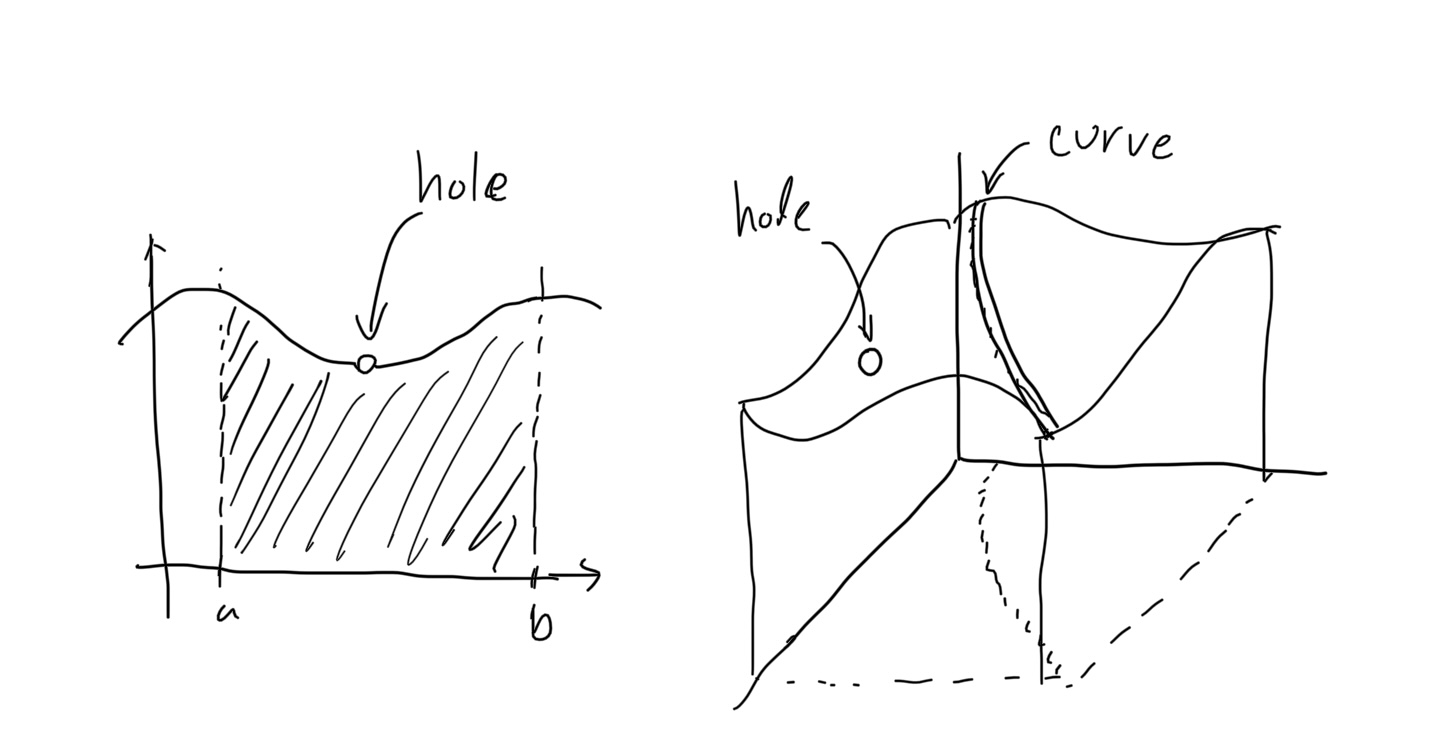
\includegraphics[scale=0.2]{img/Integrable_Hole_Function.jpg}
    \end{center}
    \item The function is defined for all values in the region, but there is a jump in the value of the function. 
    \begin{center}
        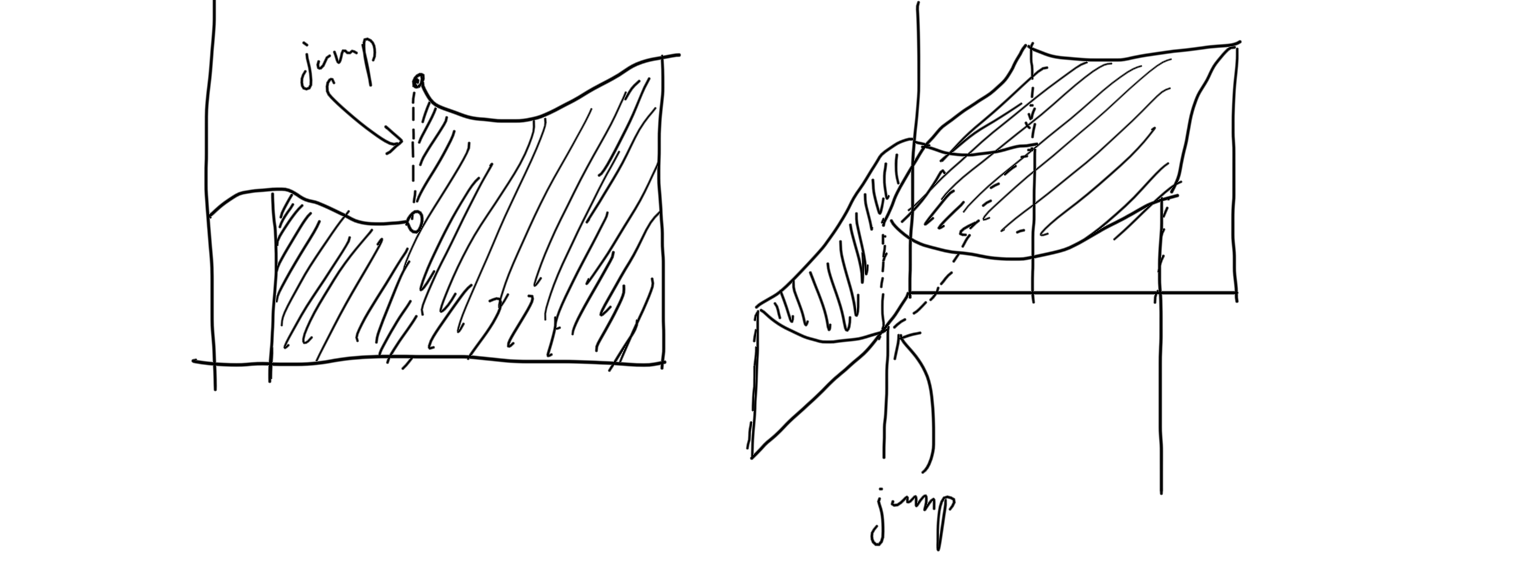
\includegraphics[scale=0.23]{img/Integrable_Jump_Function.PNG}
    \end{center}
\end{enumerate}
Informally, if we can visualize the Riemann sum converging to a well-defined area as the rectangles get thinner and thinner, then a discontinuous function is integrable. Indeed, all continuous functions (over a bounded set) are integrable since their Riemann sums are well defined. 

\subsubsection{Integration over Intervals, Rectangles, Boxes}
The simplest region that we can integrate over is a single interval 
\[B \equiv [a,b] \subset \mathbb{R}\]
a rectangle 
\[B \equiv [a, b] \times [c,d] \subset \mathbb{R}^2\]
and a box 
\[B \equiv [a,b] \times [c,d] \times [e,f] \subset \mathbb{R}^3\]
Clearly, this extends to integration over any dimension. 
\[B \equiv \prod_{i=1}^n [\alpha_i, \beta_i] \subset \mathbb{R}^n\]

Solving these integrals are quite simple. However, to rigorously define the methodology, we must use the following theorems. 

\begin{theorem}[Cavalieri's Principle]
Let $S$ be a bounded $n$-dimensional solid in $\mathbb{R}^n$ (note that $S$ can be an interval in $\mathbb{R}$). Define an $n-1$ subspace $P$ in $\mathbb{R}^n$ and given the quotient space $\mathbb{R}^n / P$ with elements $P_x$, let 
\[S \subset \bigcap_{a \leq x \leq b} P_x\]
That is, $S$ is "in between" affine subspaces $P_a$ and $P_b$. The cross section of $S$ cut by $P_x$ is the intersection of it with $S$
\[\text{Cross Section at } P_x \equiv P_x \cap S\]
Denote the area of this cross section as $A(x)$. Then, 
\[\text{Volume of } S = \int_a^b A(x) \; d x\]
\end{theorem}
This theorem basically says that the volume of $S$ is the sum of the areas of its infinitesimal cross sections. 
\begin{center}
    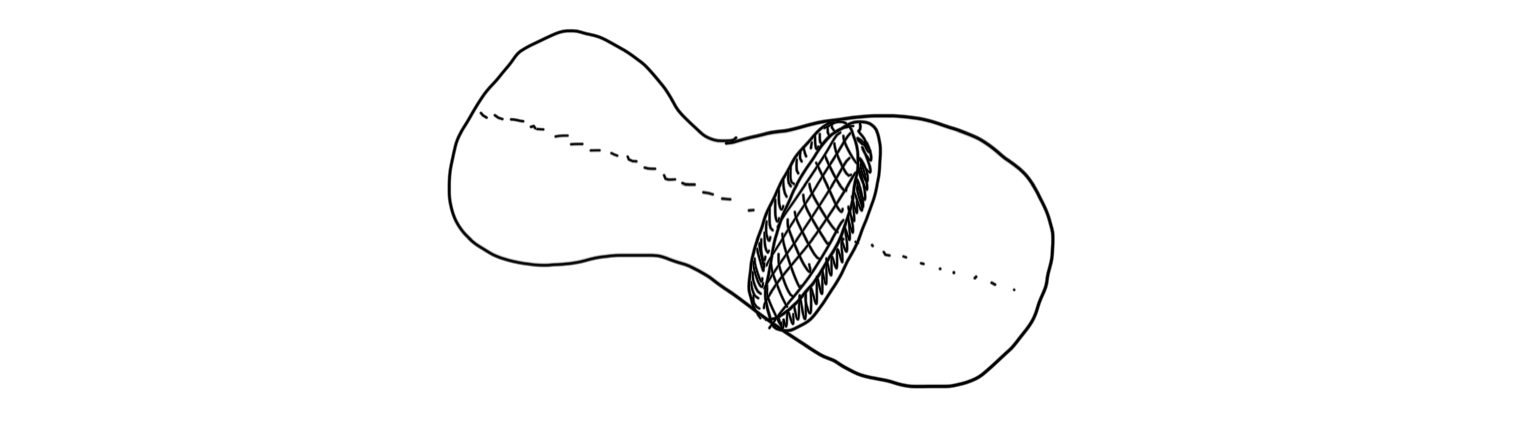
\includegraphics[scale=0.27]{img/Cavalieri_Principle .PNG}
\end{center}
This clearly works for an interval in $\mathbb{R}$, which is computed by the sum of all its "points" (rigorously speaking, infinitesimally thin intervals). The integral works for a shape in $\mathbb{R}^2$, which is computed by the sum of its "line segments" (rigorously speaking, infinitesimally thin rectangles) that add up to the shape. In $\mathbb{R}^3$, the solid is computed by the sum of its cross sections (infinitesimally thin "molded" cylinders). This analogy continues into higher dimensions. 

Given a solid $S \subset \mathbb{R}^n$, it is easy to see that no matter what subspace $P$ we choose–that is, no matter what orientation we choose to "cut" the solid– the sum of all of its cross sections should be equal to the true volume of $S$. In the case when $S$ is a box in $\mathbb{R}^n$, Fubini's theorem states that whether we cut $S$ up along the $x_1$-axis, $x_2$-axis, ..., or the $x_n$-axis, the symmetry in volume is always preserved. This theorem is really just a specific case of this general symmetry in volume. 

\begin{theorem}[Fubini's Theorem]
Given a function $f: \mathbb{R}^n \longrightarrow \mathbb{R}$, let 
\[B \equiv \prod_{i=1}^n [\alpha_i, \beta_i]\]
and let 
$p$ be any permutation of the elements $\{x_1, x_2, ..., x_n\}$. Then 
\begin{align*}
    \int_B f \; d V & = \int_{\alpha_n}^{\beta_n} ... \int_{\alpha_1}^{\beta_1} f(x_1,x_2,...,x_n) \; d x_1 ... d x_n \\
    & = \int_{p(\alpha_n)}^{p(\beta_n)} ... \int_{p(\alpha_1)}^{p(\beta_1)} f(x_1,x_2, ..., x_n) \; d p(x_1) ... d p(x_n) 
\end{align*}
In the two dimensional case, we have
\begin{align*}
    \iint_B f \; d A & = \int_c^d \int_a^b f(x, y) \; d x \, d y = \int_a^b \int_c^d f(x, y) \; d y \, d x 
\end{align*}
\begin{center}
    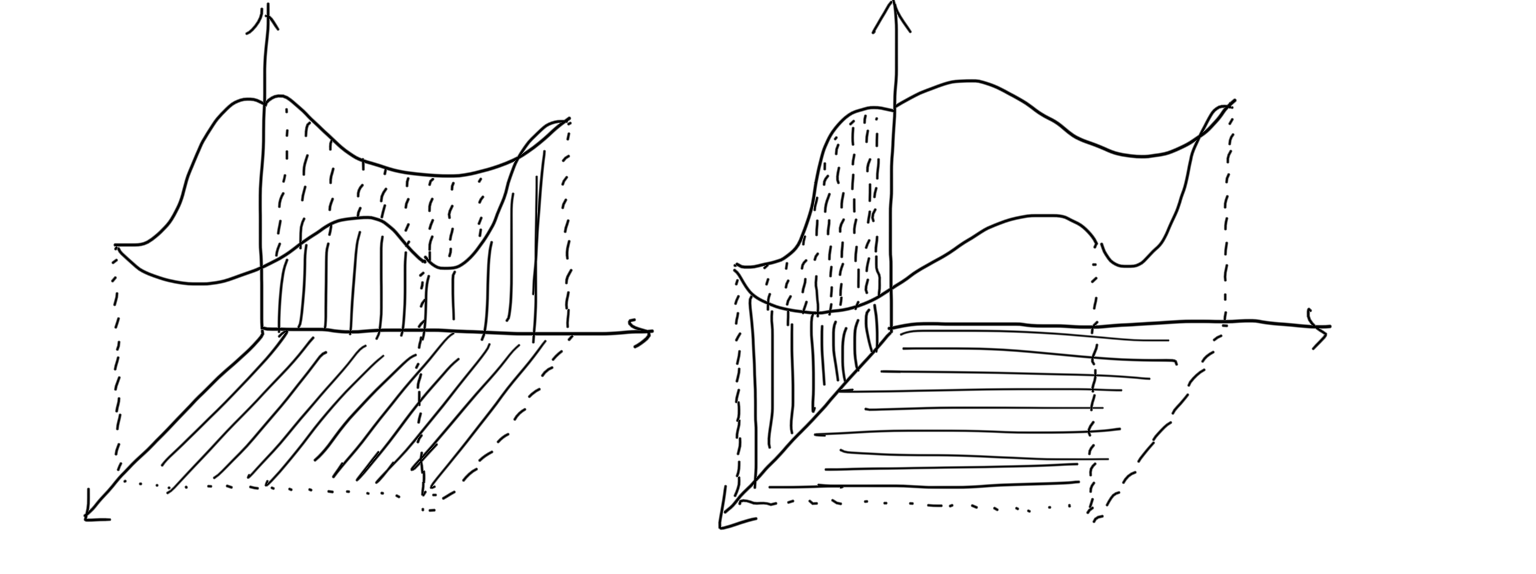
\includegraphics[scale=0.27]{img/Fubini_Theorem.PNG}
\end{center}
In the three dimensional case, we have
\begin{align*}
    \iiint_B f \; d V & 
    = \int_e^f \int_c^d \int_a^b f(x, y, z) \; d x \, d y \, d z = \int_e^f \int_a^b \int_c^d f(x, y, z) \; d y \, d x \, d z \\
    & = \int_c^d \int_a^b \int_e^f f(x, y, z) \; d z \, d x \, d y = \int_c^d \int_e^f \int_a^b f(x, y, z) \; d x \, d z \, d y \\
    & = \int_a^b \int_e^f \int_c^d f(x, y, z) \; d y \, d z \, d x = \int_a^b \int_c^d \int_e^f f(x, y, z) \; d z \, d y \, d x 
\end{align*}
\end{theorem}

Computation of these integrals is simple. You do the innermost integral first with respect to the corresponding variable, while treating the rest of the variables constant. Evaluating each integral outputs a formula for a higher dimensional cross section of the solid $S$. It is clear that computing iterated integrals is really just doing Cavalieri's principle repeatedly. 

\subsubsection{Integration over Solids Bounded by Curves}
We must first define the different types of \textit{elementary regions} first. 
\begin{definition}
A bounded region $D$ in $\mathbb{R}^n$ is said to be $x_i$-simple if it is bounded by the graphs of two continuous functions $u_1, u_2: \mathbb{R}^{n-1} \longrightarrow \mathbb{R}$ of the variables 
\[x_1, x_2, ..., x_{i-1}, x_{i+1}, ..., x_n\]
That is, $D$ can be expressed in the form 
\[\{ x \in \mathbb{R}^n \; | \; u_1 (x_1,..., x_{i-1}, x_{i+1}, ... , x_n) \leq x_i \leq u_2 (x_1, ..., x_{i-1}, x_{i+1}, ..., x_n)\}\]
If a region is simple in all of its variables, it is simply called \textit{simple}. Note that $n$-dimensional boxes are simple regions. 
\end{definition}

\begin{example}
In $\mathbb{R}^2$, the region on the left graph is an $y$-simple region and the region on the right is a $x$-simple region. 
\begin{center}
\begin{tikzpicture}[scale=0.8]
  \draw[<->] (-1,0)--(5,0);
  \draw[<->] (0,-1)--(0,5);
  \draw[<->] (6,0)--(12,0);
  \draw[<->] (7,-1)--(7,5);
  \draw plot [smooth] coordinates {(0.6, 1.2) (1,1) (2,1.4) (3,1.3) (4,1.5) (4.3,1.7)};
  \draw plot [smooth] coordinates {(0.6, 3.9) (1,4.1) (2,4) (3,4.3) (4,4.2) (4.3,4.1)};
  \draw[dashed] (0.6,1.2)--(0.6,3.9);
  \draw[dashed] (4.3,1.7)--(4.3,4.1);
  \draw plot [smooth] coordinates {(8.2,0.6) (8,1) (8.4,2) (8.3,3) (8.5,4) (8.7,4.3)};
  \draw plot [smooth] coordinates {(10.9,0.6) (11.1,1) (11,2) (11.3,3) (11.2,4) (11.1,4.3)};
  \draw[dashed] (8.2,0.6)--(10.9,0.6);
  \draw[dashed] (8.7,4.3)--(11.1,4.3);
  \node[below] at (4.8,0) {$x$};
  \node[below] at (11.8,0) {$x$};
  \node[left] at (0,4.8) {$y$};
  \node[left] at (7,4.8) {$y$};
  \node[above] at (3,4.2) {$u_1$};
  \node[above] at (3,1.3) {$u_2$};
  \node[left] at (8.3, 3) {$v_1$};
  \node[right] at (11.3, 3) {$v_2$};
  \draw[fill] (0.6,0) circle (0.05);
  \node[below] at (0.6,0) {$a$};
  \draw[fill] (4.3,0) circle (0.05);
  \node[below left] at (4.3,0) {$b$};
  \draw[fill] (7,0.6) circle (0.05);
  \draw[fill] (7,4.3) circle (0.05);
  \node[left] at (7,0.6) {$c$};
  \node[left] at (7,4.3) {$d$};
\end{tikzpicture}
\end{center}
\end{example}
We now describe the method of calculating double integrals over elementary regions. 
\begin{theorem}
The double integral over a $y$-simple region $D$ bounded by functions $u_1$ and $u_2$ in $\mathbb{R}^2$ and the $x$-values $a$ and $b$ (as shown in the left graph of example 2.1) is
\[\iint_D f(x, y) = \int_a^b \int_{u_2 (x)}^{u_1 (x)} f(x, y) \, dy \, dx\]
The double integral over an $x$-simple region $D$ bounded by functions $v_1$ and $v_2$ in $\mathbb{R}^2$ and the $y$-values $c$ and $d$ (shown in the right of graph of example 2.1) is 
\[\iint_D f(x, y) = \int_c^d \int_{v_2 (y)}^{v_1 (y)} f(x, y) \, dx \, dy\]
\end{theorem}

\begin{example}
Integrating $f(x, y)$ over the unit disk would have the form
\[\int_{-1}^1 \int_{-\sqrt{1-x^2}}^{\sqrt{1-x^2}} f(x,y) \, dy\, dx \text{ or } \int_{-1}^1 \int_{-\sqrt{1-y^2}}^{\sqrt{1-y^2}} f(x,y) \, dx\, dy \]
Note that the unit disk is both $x$ and $y$ simple. 
\end{example}
\subsection{Change of Basis}
Sometimes, integrating a region over a different basis would make the integral computation much more simpler. In this case, we may be able to transform more complicated regions into elementary regions. We first introduce a change of basis in 2 dimensions and then generalize it into higher dimensions. 
\\
Let $\mathbb{R}^2$ have the standard orthonomal basis $e_1, e_2$, commonly known as the $x, y$ basis. Now, let us construct new basis vectors of $\mathbb{R}^2$, denoted $f_1, f_2$ such that $f_1, f_2$ are functions of $e_1, e_2$. Since they are both bases that span $\mathbb{R}^2$, we can equally represent $e_1, e_2$ as functions of $f_1, f_2$. 
\begin{align*}
    &e_1 = g(f_1, f_2)\\
    &e_2 = h(f_1, f_2) 
\end{align*}
Note that this change of basis does not necessarily have to be linear, as in the context of passive transformation in linear algebra. Then, every point $(x,y)$ in the $(e_1, e_2)$-basis can be rewritten as
\begin{align*}
    (x, y) & = x e_1 + y e_2 \\
    & = x \, g(f_1, f_2) + y \, h(f_1, f_2) \\
    & = u f_1 + v f_2
\end{align*}
Note that it is customary to denote $x, y$ as the coefficients in the $e_1, e_2$ basis and $u, v$ as the coefficients in the new $f_1, f_2$ basis. This way, we can not only write $e_1$ and $e_2$ as functions of $f_1$ and $f_2$, but we can also write the coefficents $x, y$ as functions of the coeffiecents $u, v$! That is, 
\begin{align*}
    & x = x(u, v) \\
    & y = y(u, v)
\end{align*}
which is really just a function 
\[B: \mathbb{R}^2 \longrightarrow \mathbb{R}^2, \;\; B(u, v) = \begin{pmatrix} x(u, v) \\ y(u, v) \end{pmatrix}\]
Notice that $B$ changes the $u, v$ coordinates to the $x, y$ coordinates, and $B^{-1}$ changes the $x, y$ coordinates to the $u, v$ coordinates. 
\[B^{-1}: \mathbb{R}^2 \longrightarrow \mathbb{R}^2, \;\; B^{-1} (x, y) = \begin{pmatrix} u (x, y) \\ v (x, y) \end{pmatrix}\]
Note that these coefficients actually change \textit{contravariantly}, that is, they change inversely with respect to how the basis vectors are changed. In vector calculus, it is conventional to represent a change of basis with functions that relate the coefficients $x, y$ with $u, v$, rather than the bases $f_1, f_2$ with $e_1, e_2$. 

\begin{theorem}[Integration over Change of Bases in $\mathbb{R}^2$]
Let $\mathbb{R}^2$ have the standard orthonomal basis $e_1, e_2$. Now, let us construct new basis vectors of $\mathbb{R}^2$, denoted $f_1, f_2$ such that the coefficients of the vectors in $\mathbb{R}^2$ are related by the change of basis function 
\[B = \begin{pmatrix} x \\ y \end{pmatrix} \implies B(u, v) = \begin{pmatrix} x(u, v) \\ y(u, v) \end{pmatrix}\]
Given region $D \subset \mathbb{R}^2$ and $S = B(D)$ is the region transformed by $B$, the integral of function $f(x, y)$ over region $D$ can be expressed as 
\[\iint_D f(x, y) \, dA = \iint_S f \big( x(u, v), y(u, v) \big) \, \big| J B(u, v) \big| \, d \bar{A}\]
where $\big| J B(u, v) \big|$ is the determinant of the Jacobian matrix of $B$. Expanding the Facobian determinant gives
\[\big| J B(u, v) \big| = \frac{\partial x}{\partial u} \frac{\partial y}{\partial v} - \frac{\partial x}{\partial v} \frac{\partial y}{\partial u}\]
\end{theorem}

\begin{theorem}[Integration over Change of Bases in $\mathbb{R}^3$]
Given that we have the change of basis function 
\[B: \mathbb{R}^3 \longrightarrow \mathbb{R}^3, \;\;\; B(u, v, w) = \begin{pmatrix} x(u, v, w) \\ y(u, v, w) \\ z(u, v, w) \end{pmatrix}\]
a region $D \in \mathbb{R}^3$ and $S = B(D)$, the region transformed by $B$, the integral of $f(x, y, z)$ over region $D$ can be expressed as 
\[\iiint_D f(x, y, z)\, dV = \iiint_S f\big( x(u, v, w), y(u, v ,w), z(u, v, w) \big) \big| J B (u, v, w)\big| \, d \bar{V}\]
where $\big| J B (u, v, w)\big|$ is the Jacobian determinant of $B$. 
\end{theorem}

\begin{example}
Given a real-valued function $f$ defined over the region $D \subset \mathbb{R}^2$, we can perform a change of basis of the $x, y$ coordinates into polar ones within a new region $S$. The change of basis 
\begin{align*}
    & x = r \cos{\theta} \\
    & y = r \sin{\theta} 
\end{align*}
\begin{center}
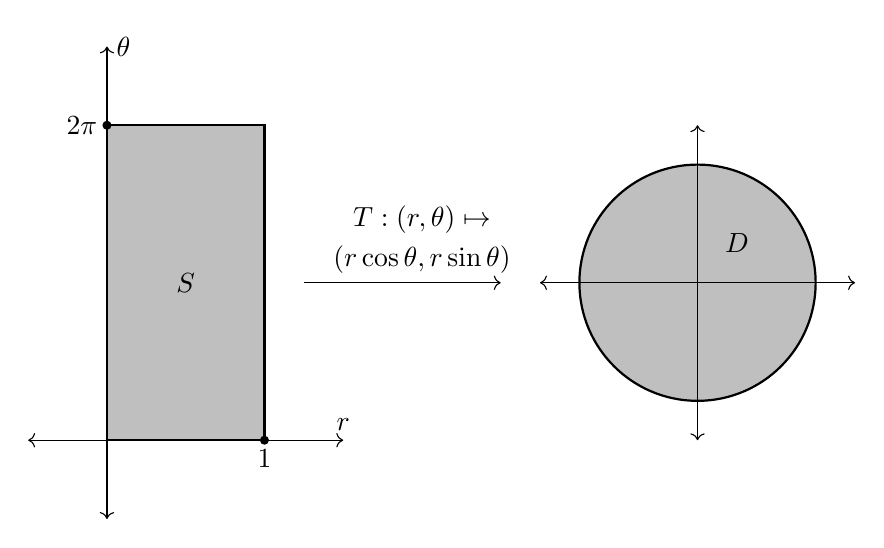
\begin{tikzpicture}
    \draw[thick, fill=lightgray] (7.5,2) circle (1.5);
    \draw[<->] (-1,0)--(3,0);
    \draw[<->] (0,-1)--(0,5);
    \draw[thick, fill=lightgray] (0,0) rectangle (2,4);
    \node at (1,2) {$S$};
    \draw[fill] (0,4) circle (0.05);
    \draw[fill] (2,0) circle (0.05);
    \node[below] at (2,0) {$1$};
    \node[left] at (0,4) {$2 \pi$};
    \node[above] at (3,0) {$r$};
    \node[right] at (0,5) {$\theta$};
    \draw[->] (2.5, 2)--(5,2);
    \node[above] at (4,2.5) {$T: (r, \theta) \mapsto$};
    \node[above] at (4,2) {$ (r \cos{\theta}, r \sin{\theta})$};
    \draw[<->] (5.5,2)--(9.5,2);
    \draw[<->] (7.5,0)--(7.5,4);
    \node at (8,2.5) {$D$};
\end{tikzpicture}  
\end{center}
\end{example}

\begin{theorem}[Integration over Change of Bases in $\mathbb{R}^n$]
Let $\mathbb{R}^n$ have the standard orthonormal basis $e_1, e_2, ..., e_n$, and let us construct a new basis $f_1, f_2, ..., f_n$ such that the coefficients of the vectors in $\mathbb{R}^n$ are related with the functions
\[B: \mathbb{R}^n \longrightarrow \mathbb{R}^n, \;\;\;\; B(u_1, u_2, \ldots, u_n) = \begin{pmatrix}
x_1 (u_1, \ldots, u_n) \\x_2 (u_1, \ldots, u_n) \\ \vdots \\ x_n (u_1, \ldots, u_n)
\end{pmatrix}\]
Given that the region $D \subset \mathbb{R}^n$ is transformed into a new region $S = B(D) \subset \mathbb{R}^n$ under this basis transformation, the integral of function $f(x_1, \ldots, x_n)$ over region $D$ can be expressed as 
\[\int_D f(x) \, dH = \int_S f \big( x_1(u), x_2(u), ..., x_n (u) \big) \big| J B(u_1, \ldots, u_n)\big| \, d \bar{H}\]
where the integral on both the left and right hand side represents integration over an $n$-dimensional region, $x$ represents the $n$-tuple $(x_1, \ldots, x_n)$, $u$ represents the $n$-tuple $(u_1, \ldots, u_n)$, and $\big| J B(u_1, \ldots, u_n)\big|$ represents the Jacobian determinant of function $B$. 
\end{theorem}

We now describe some common change of basis formulas for polar, cylindrical, and spherical coordinates. 

\begin{theorem}[Integration in Polar Coordinates]
\[\iint_{D} f(x, y) \, dx \,dy = \iint_S f(r \cos{\theta}, r \sin{\theta}) r \, dr \, d\theta\]
\end{theorem}

\begin{definition}[Cylindrical, Spherical Coordinates]
In $\mathbb{R}^3$, \textit{cylindrical coordinates} have the following relation to rectangular coordinates. 
\begin{align*}
    & x = r \cos{\theta} \\
    & y = r \sin{\theta} \\
    & z = z
\end{align*}
In $\mathbb{R}^3$, \textit{spherical coordinates} have the following relation to rectangular coordinates. 
\begin{align*}
    & x = \rho \sin{\phi} \cos{\theta} \\
    & y = \rho \sin{\phi} \sin{\theta} \\
    & z = \rho \cos{\phi}
\end{align*}
\end{definition}

\begin{corollary}[Integration in Cylindrical Coordinates]
\[\iiint_D f(x, y, z) \, dx \, dy \, dz = \iiint_S f( r \cos{\theta}, r \sin{\theta}, z) r \, dr \, d\theta \, dz\]
\end{corollary}

\begin{corollary}[Integration in Spherical Coordinates]
\[\iiint_D f(x, y, z) \,dx\,dy\,dz = \iiint_S f(\rho \sin{\phi} \cos{\theta}, \rho \sin{\phi} \sin{\theta}, \rho \cos{\phi}) \rho^2 \sin{\theta} \, d\rho \, d\theta \, d\phi\]
\end{corollary}

\begin{example}[Gaussian Integral]
The following is the (un-normalized) probability distribution function of the Gaussian distribution. 
\[\int_{-\infty}^{\infty} e^{-x^2} \, dx = \sqrt{\pi}\]
\end{example}

\subsection{Average Values, Centers of Mass}
\begin{definition}
The \textit{average value} of a function defined over a region $D \subset \mathbb{R}^n$ is 
\[[f]_{av} = \bigg(\int_D f(x) \,d V \bigg) \bigg/ \bigg( \int_D \, d V \bigg) \]
where both integrals represent integration over the $n$-dimensional region $D$. Informally, the integral above represents the infinitesimal sum of all the values of the function $f$ over $D$ and divides it by the hypervolume of $D$ to average it out. More specifically, the average value of $f: \mathbb{R} \longrightarrow \mathbb{R}$ in the interval $[a,b]$ is defined
\[ [f]_{av} = \bigg(\int_a^b f(x) \,d x \bigg) \bigg/ \bigg( \int_a^b \, d x \bigg) = \frac{1}{b-a} \int_a^b f(x) \,d x \]
For a function $f: \mathbb{R}^2 \longrightarrow \mathbb{R}$ over a two dimensional region $D$, we have 
\[[f]_{av} = \bigg(\iint_D f(x, y) \,dx\,dy \bigg) \bigg/ \bigg( \iint_D \, dx\,dy \bigg)\]
For $f: \mathbb{R}^3 \longrightarrow \mathbb{R}$ over a three dimensional region $V$, we have
\[[f]_{av} = \bigg(\iiint_V f(x, y, z) \,dx\,dy\,dz \bigg) \bigg/ \bigg( \iiint_V \, dx\,dy\,dz \bigg)\]
\end{definition}

It is quite easy to get the center of mass of a system of $n$-distinct points in $\mathbb{R}^n$. We can solve each $x_i$ coordinate for the center of mass by averaging out the $x_i$ coordinates scaled by their respective masses. That is, given points $x_1, x_2, ..., x_n$ with respective masses $m_1, ..., m_n$, the center of mass is defined as
\[\bar{x} = \frac{\sum m_i x_i}{\sum m_i}\]

\begin{definition}
Given an $n$-dimensional continuous mass density distribution, denoted $\delta(x)$, defined over a region $D \subset \mathbb{R}^n$, the center of mass of $D$ can be determined through coordinates.
\[\bar{x_i} = \bigg( \int_D x_i \, \delta(x) d V\bigg) \bigg/ \bigg(\int_D \delta(x) d V \bigg), \; i = 1, 2, 3, ..., n\]
Note that $\delta$ must be continuous (in order for it to be integrable). More specifically, the center of mass of a one dimensional interval $I \subset \mathbb{R}$ is
\[\bar{x} = \bigg(\int_I x\, \delta(x) \, dx\bigg) \bigg/ \bigg(\int_I \delta(x) \, dx\bigg)\]
For a two dimensional region (which we can visualize as a "disk" or "plate," the $x$ and $y$ coordinates for the center of mass is
\begin{align*}
    & \bar{x} = \bigg(\iint_D x\, \delta(x, y) \, dx\,dy\bigg) \bigg/ \bigg(\iint_D \delta(x, y) \, dx\,dy \bigg) \\
    & \bar{y} = \bigg(\iint_D y\, \delta(x, y) \, dx\,dy\bigg) \bigg/ \bigg(\iint_D \delta(x, y) \, dx\,dy \bigg)
\end{align*}
For a three dimensional mass, the $x, y, z$ coordinates of the center of mass of volume $V$ can be found with
\begin{align*}
    & \bar{x} = \bigg(\iiint_V x\, \delta(x, y, z) \, dx\,dy\,dz\bigg) \bigg/ \bigg(\iiint_V \delta(x, y, z) \, dx\,dy \,dz\bigg) \\
    & \bar{y} = \bigg(\iiint_V y\, \delta(x, y, z) \, dx\,dy\,dz\bigg) \bigg/ \bigg(\iint_V \delta(x, y, z) \, dx\,dy\,dz \bigg) \\
    & \bar{z} = \bigg(\iiint_V z\, \delta(x, y, z) \, dx\,dy\,dz\bigg) \bigg/ \bigg(\iint_V \delta(x, y, z) \, dx\,dy\,dz \bigg)
\end{align*}
\end{definition}

\subsection{Improper Integrals}
There are generally two types of improper integrals. 
\begin{enumerate}
    \item The region $D$ integrated over is unbounded. 
    \item The function $f$ that is integrated is unbounded within the region $D$.
\end{enumerate}
\subsubsection{Single Variable Improper Integrals}
These types of improper integrals are usually evaluated using a limiting process. When the interval $I$ is unbounded, say $(1, \infty)$, the integral can be evaluated as 
\[\int_1^\infty \frac{1}{x^2} \,dx = \lim_{b \rightarrow \infty} \int_1^b \frac{1}{x^2} \, dx = \lim_{b\rightarrow \infty} \bigg( 1 - \frac{1}{b} \bigg) = 1\]
In case 2, we can add a limit at the point where the function $f$ diverges as such. 
\[\int_0^1 \frac{1}{\sqrt{x}} \, dx = \lim_{a \rightarrow 0} \int_a^1 \frac{1}{\sqrt{x}} \, dx = \lim_{a \rightarrow 0} (2 - 2\sqrt{a}) = 2\]
We now describe how to integrate over a certain path $p$ embedded in a higher dimensional space $\mathbb{R}^n$, possibly with a scalar or vector field $f$. We must first go over oriented paths. 

\subsubsection{Two Variable Improper Integrals}
Extending the previous case, we use a multivariate limiting process in $\mathbb{R}^2$. We will first work with case 2, when $f$ is unbounded within the region $D$. Let us define an elementary region $D$ in $\mathbb{R}^2$; without loss of generality, we will make it $y$-simple, meaning that $D$ can be expressed as
  \[D \equiv \{ (x, y) \in \mathbb{R}^2 \; | \; a \leq x \leq b, \; \phi_1 (x) \leq y \leq \phi_2 (x)\}\]
We can actually assume that the region in which $f$ is unbounded lies in the boundary $\partial D$. This is because if it lied in the interior of $D$, we could split $D$ into pieces across a path that intersects this region with divergent values, evaluate the integrals over the pieces separately, and then sum the integrals. For example, in the rectangular region below, let the dashed line represent the values where the function $f$ diverges. Then, we can split the region into two rectangular regions shown in the right. 
\begin{center}
\begin{tikzpicture}
  \draw (0,0) rectangle (3,2);
  \draw[dashed] rectangle (2,0)--(2,2);
  \draw[->] (3.5,1)--(5,1);
  \draw (8,0)--(6,0)--(6,2)--(8,2);
  \draw[dashed] (8,0)--(8,2);
  \draw[dashed] (9,0)--(9,2);
  \draw (9,0)--(10,0)--(10,2)--(9,2);
\end{tikzpicture}
\end{center}
Therefore, assuming that $f$ is unbounded in $\partial D$, we can construct a new region 
\[D_{\eta, \delta} \equiv \{(x, y) \in \mathbb{R}^2 \; | \; a + \eta \leq x \leq b - \eta, \; \phi_1 (x) + \delta \leq y \leq \phi_2 (x) - \delta\}\]
for some arbitrarily small numbers $\eta, \delta >0$, meaning that the integral (reduced to iterated integrals using Fubini's theorem) 
\[F(\eta, \delta) \equiv \iint_{D_{\eta, \delta}} f(x, y) \, dA = \int_{a + \eta}^{b - \eta} \int_{\phi_1 (x) + \delta}^{\phi_2 (x) - \delta} f(x, y) \, dy\,dx\]
is well defined. 
\begin{center}
\begin{tikzpicture}
    \draw[<->] (-0.5,0)--(5,0);
    \draw[<->] (0,-0.5)--(0,5);
    \draw (1,1.5)--(1,3);
    \draw plot [smooth] coordinates {(1,3) (1.5,3.3) (2,3.1) (3,3.8) (4,4.2) (4.5,4)};
    \draw (4.5, 4)--(4.5,1);
    \draw plot [smooth] coordinates {(1,1.5) (2,1.7) (3, 1.6) (3.7, 1.3) ( 4.5,1)};
    \draw[dashed] (1.3,1.85)--(1.3,2.9);
    \draw[dashed] (4.2, 3.8)--(4.2,1.4);
    \draw[dashed] plot [smooth] coordinates {(1.3,2.9) (1.5,3) (2,2.8) (3,3.5) (4,3.9) (4.2,3.8)};
    \draw[dashed] plot [smooth] coordinates {(1.3,1.85) (2,2) (3, 1.9) (3.7, 1.6) ( 4.2,1.4)};
    \node at (3,2.5) {$D_{\eta, \delta}$};
    \node[below left] at (2,1) {$D$};
    \draw[->] (2,1)--(2.5,1.85);
\end{tikzpicture}
\end{center}
Clearly, the function $F( \eta, \delta)$ is a function of two variables $\eta$ and $\delta$. So, if the limit 
\[\lim_{(\eta, \delta) \rightarrow (0, 0)} F(\eta, \delta)\]
is well defined, then so is the improper integral. For it to exist, the iterated limits must both equal to a well-defined real number $\mathcal{L}$ (and to each other). That is, 
\[\lim_{\eta \rightarrow 0} \lim_{\delta \rightarrow 0} F(\eta, \delta) = \lim_{\delta \rightarrow 0} \lim_{\eta \rightarrow 0} F(\eta, \delta) = \mathcal{L} \implies \lim_{(\eta, \delta) \rightarrow (0,0)} F(\eta, \delta) = \mathcal{L}\]


It is also worthwhile to note that functions unbounded at isolated points can be evaluated using the methods above using a change of basis. Consider the example below. 

\begin{example}
In the unit disk $D \subset \mathbb{R}^2$, let the function $f$ be defined as 
\[f(x, y) \equiv \frac{1}{\sqrt{x^2 + y^2} }\]
Clearly, $f$ is continuous at every point except $0= (0,0)$, meaning that 
\[\iint_{D \setminus \{0\}} f(x, y)\, dA\]
is well-defined. In order to solve the integral over the entire disk, we convert to polar coordinates and evaluate the limit
\[\iint_{D \setminus \{0\}} f(x, y) \, dA = \lim_{\delta \rightarrow 0} \int_{\delta}^1 \int_0^{2 \pi} r \, f( r \cos{\theta}, r \sin{\theta}) \, d\theta \,dr\]
\end{example}
\begin{center}
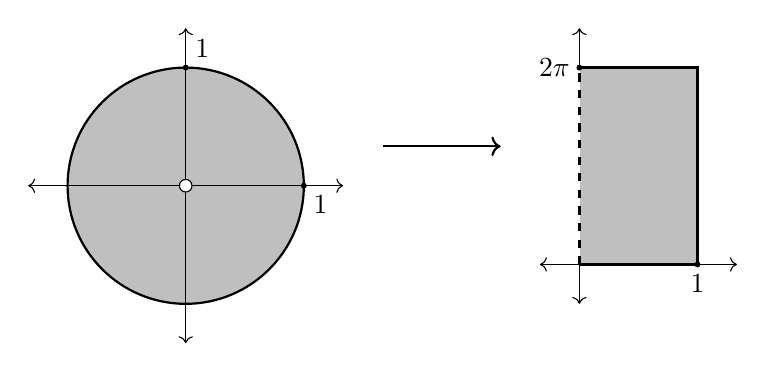
\begin{tikzpicture}
    \draw[thick, fill=lightgray] (0,0) circle (1.5); 
    \draw[<->] (-2,0)--(2,0);
    \draw[<->] (0,-2)--(0,2);
    \draw[fill=white] (0,0) circle (0.08);
    \draw[->, thick] (2.5,0.5)--(4, 0.5); 
    \draw[<->] (4.5,-1)--(7,-1);
    \draw[<->] (5,-1.5)--(5,2);
    \draw[white, fill=lightgray] (5,-1) rectangle (6.5,1.5);
    \draw[thick] (5,-1)--(6.5,-1)--(6.5,1.5)--(5,1.5);
    \draw[thick, dashed] (5,-1)--(5,1.5);
    \draw[fill] (6.5,-1) circle (0.03);
    \node[below] at (6.5,-1) {$1$};
    \node[left] at (5,1.5) {$2 \pi$};
    \draw[fill] (5, 1.5) circle (0.03);
    \draw[fill] (1.5,0) circle (0.03);
    \draw[fill] (0,1.5) circle (0.03);
    \node[below right] at (1.5,0) {$1$};
    \node[above right] at (0,1.5) {$1$};
\end{tikzpicture}
\end{center}

If we are given an unbounded region $D \subset \mathbb{R}^2$, we can first create a bounded region and expand that region using a limit to cover all of $D$. 

\subsection{Line Integrals}
\begin{definition}[Orientations, Simple Curves, Closed Curves]
A path function $p: [a,b]\subset \mathbb{R} \longrightarrow \mathbb{R}^n$ determines a curve in $\mathbb{R}^n$ with endpoints $p(a)$ and $p(b)$. The direction the curve $p$ takes, that is from $p(a)$ to $p(b)$ in $\mathbb{R}^n$ is called the \textit{orientation} of $p$. A path or a curve with a defined orientation is called an \textit{oriented curve}. 

A \textit{simple curve} $C$ to be the image of an injective piecewise $C^1$ map $c: I \subset \mathbb{R} \longrightarrow \mathbb{R}^3$. Since it is inejctive, it does not intersect itself, and $C$ is piecewise smooth in $\mathbb{R}^n$. If $I = [a,b]$, then $c(a)$ and $c(b)$ are the endpoints of the curve. A simple curve with an orientation is called an \textit{oriented simple curve}. 

A closed curve $C$ is the image of piecewise $C^1$ map $c: [a,b] \longrightarrow \mathbb{R}^n$ such that $c(a) = c(b)$. That is, the endpoints of $C$ are equal. A \textit{simple closed curve} is a closed curve that is injective over the interval $[a,b)$. Note that a closed curve has two possible orientations. 
\end{definition}

If $C$ is an oriented simple curve or an oriented simple closed curve, then we can unambiguously define line integrals along them. 

\begin{definition}
Let $h$ be an injective function that takes $[\alpha,\beta] \subset \mathbb{R}$ to the interval $[a, b] \subset \mathbb{R}$. Given an oriented simple path function $p: [a,b]\subset \mathbb{R} \longrightarrow \mathbb{R}^n$, the composition
\[\rho = p \circ h: [\alpha, \beta] \longrightarrow \mathbb{R}^n\]
is called a \textit{reparamaterization} of $p$. Note that since $h$ is injective, it takes endpoints to endpoints. If $h$ preserves the direction in which the path travels, that is, if 
\[(p \circ h)(\alpha) = a \text{ and } (p \circ h)(\beta) = b\]
then $h$ is \textit{orientation preserving}. If
\[(p \circ h)(\alpha) = b \text{ and } (p \circ h)(\beta) = a\]
then $h$ is \textit{orientation reversing}. Note that a path $c$ having the same image as $p$ does not imply that $c$ is a reparamaterization of $p$, since $c$ may not be injective. 
\begin{center}
    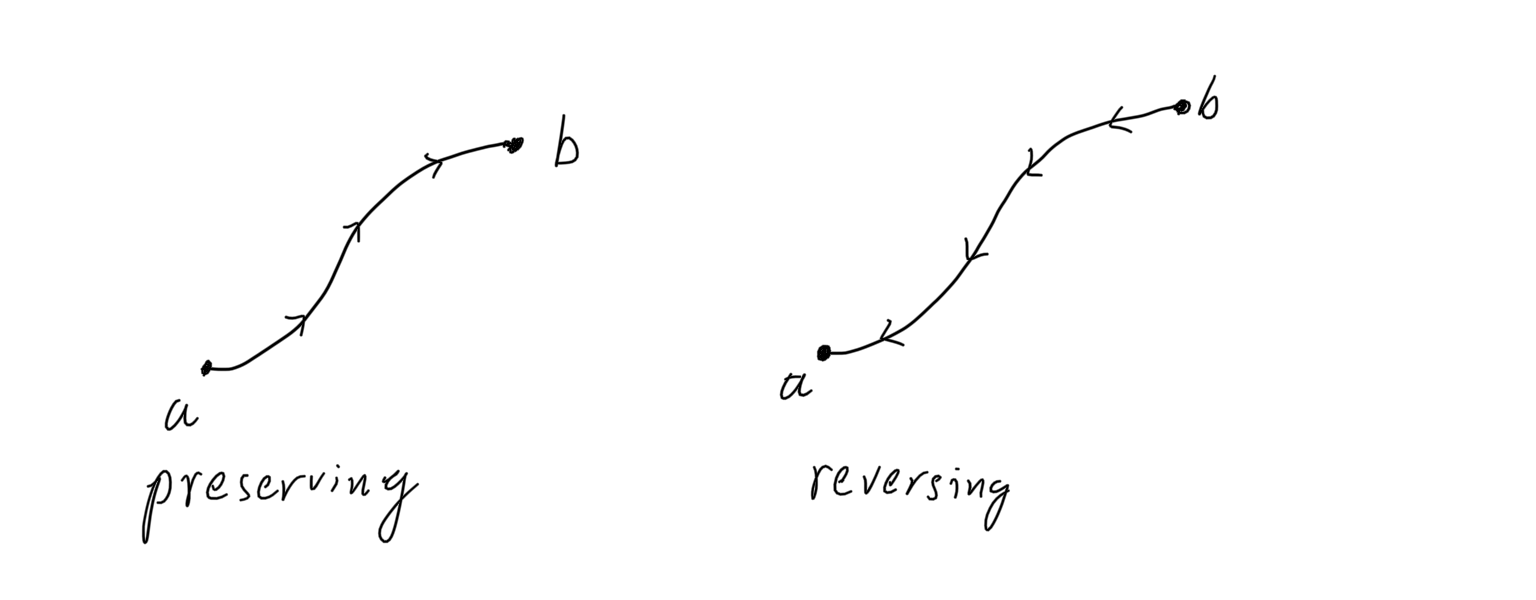
\includegraphics[scale=0.25]{img/Orientation_Preserving_Reversing.PNG}
\end{center}
\end{definition}

\begin{definition}[Scalar Line Integral]
Let $f: \mathbb{R}^n \longrightarrow \mathbb{R}$, which can be interpreted as a scalar field. Now define a $C^1$ path function 
\[c: [a,b] \subset \mathbb{R} \longrightarrow \mathbb{R}^n \]
such that the composition of functions
\[f \circ c: [a, b] \subset \mathbb{R} \longrightarrow \mathbb{R}^n\]
is continuous. Then, the \textit{path integral}, or \textit{scalar line integral}, of $f$ along the path $c$. is defined
\begin{align*}
    \int_c f \;d s & = \int_a^b f\big(c(t)\big) ||c^\prime (t)|| \;d t \\
    & = \int_a^b f\big( x_1 (t), x_2 (t), ..., x_n (t)\big) ||c^\prime (t)|| \; d t
\end{align*}
If $c(t)$ is only piece-wise $C^1$, we can define the path integral by breaking $[a,b]$ into pieces over with $f\big( c(t)\big) ||c^\prime (t)||$ is continuous and then summing the integrals over the pieces. 
That is, 
\[\int_a^b f\big(c(t)\big) ||c^\prime (t)|| \;d t = \sum_{i = 0}^{n-1} \int_{\alpha_i}^{\alpha_{i+1}} f\big(c(t)\big) ||c^\prime (t)|| \; d t\]
\end{definition}
Note that since $f$ is a scalar-valued function, we can interpret a path integral as the sum of infinitesmal segments of the path $c$ having a weight determined by $f$ at each section. 
If $f$ is a constant function outputting $1$ at every point, then the path integral just outputs the length of the path $c$ in $\mathbb{R}^n$. 
\[L = \int_a^b f\big( c(t)\big) ||c^\prime (t)|| \; d t = \int_a^b ||c^\prime (t)|| \; d t\]

\begin{definition}[Vector Line Integral]
Let $F: \mathbb{R}^n \longrightarrow \mathbb{R}^n$ be a vector field on $\mathbb{R}^n$ that is continuous on the $C^1$ oriented path $c: [a, b] \subset \mathbb{R} \longrightarrow \mathbb{R}^n$. The \textit{line integral} of $F$ along $c$ is defined by the formula 
\[\int_c F \cdot d s = \int_a^b F\big( c(t)\big) \cdot c^\prime (t) \; d t\]
where $\cdot$ represents the dot product of $F$ with $c^\prime$ over the interval $[a,b]$. It is also commonly written in differential notation, 
\[\int_c F \cdot ds = \int_c F \cdot (dx_1, \ldots, d x_n) = \int_c F_1 dx_1 + F_2 dx_2 + \ldots F_n dx_n\]
\begin{center}
    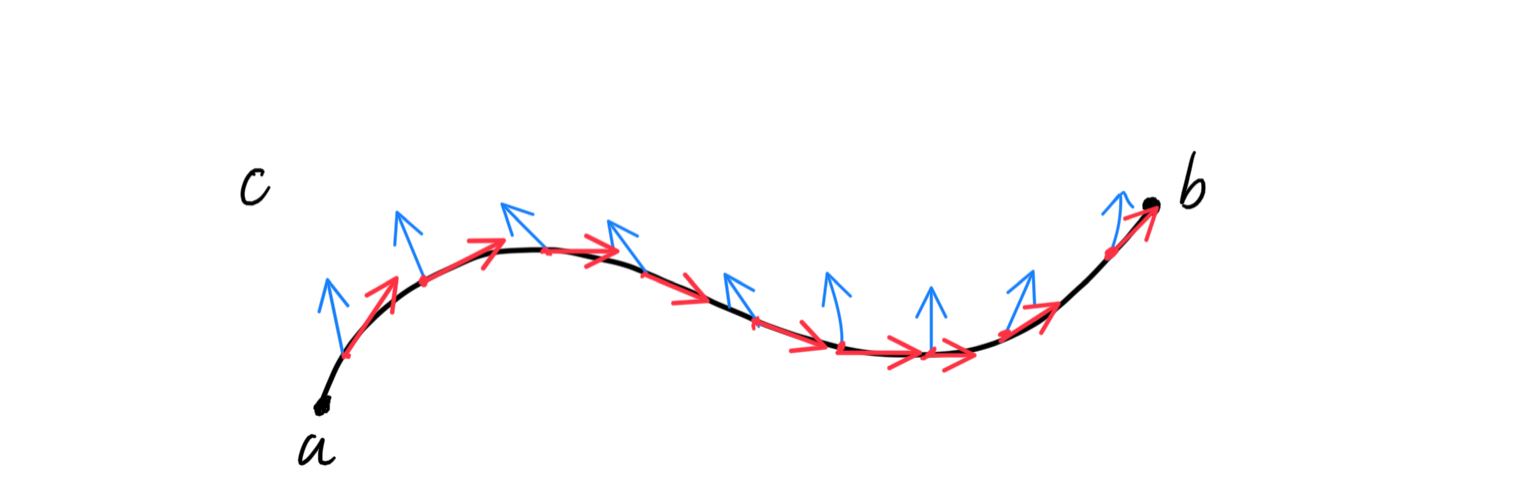
\includegraphics[scale=0.27]{img/Vector_Line_Integral.PNG}
\end{center}
 Similarly with path integrals, we can also define line integrals as the sum of integrals over piece-wise continuous sections of $c$. That is, given an oriented curve $C$ made up of several oriented component curves $C_i$, $i = 1, 2, ..., k$, we can paramaterize $C$ by paramaterizing the pieces $C_i$'s separately. Thus, we can treat $C = C_1 + ... C_k$ and get
\[\int_C F \cdot d s = \sum_{i = 1}^k \int_{C_i} F \cdot d s\]
Note that a vector line integral is a generalization of scalar line integrals, so any results holding for vector line integrals also holds for their scalar counterpart. 
\end{definition}

\begin{example}[Work]
In mechanics, work $W$ is defined as 
\[W = F \cdot d\]
where $F$ is force and $d$ is displacement. With this knowledge, the reader can easily see that the work done by vector field $F$ on a particle traveling along a path $c$ from time $a$ to time $b$ can be calculated by the line integral
\begin{align*}
    W & = \int_a^b F\big( c(t)\big) \cdot c^\prime (t) \; d t \\
    & = \int_c F_1 dx + F_2 dy + F_3 dz
\end{align*}
\end{example}

\begin{theorem}[Invariance of Path Paramaterizations on Vector Line Integrals]
Let $F$ be a vector field and $f$ be a scalar field, both continuous on the $C^1$ path function $p: [a,b] \longrightarrow \mathbb{R}^n$ and let $q: [\alpha, \beta] \longrightarrow \mathbb{R}^n$ be a reparamaterization of $p$. Then, 
\begin{align*}
    q \text{ is orientation preserving} & \implies \int_p F \cdot d s = \int_q F \cdot d s \\
    q \text{ is orientation reversing} & \implies \int_p F \cdot d s = - \int_q F \cdot d s
\end{align*}
\end{theorem}

\subsubsection{Conservative Vector Fields}
We now introduce a fundamental theorem about line integrals over gradient fields. Recall the fundamental theorem of calculus and it's equivalent form. 

\begin{theorem}[Fundamental Theorem of Single Variable Calculus]
Let function $\nabla g: \mathbb{R} \longrightarrow \mathbb{R}$ be the gradient of the single variable $C^1$ function $g: \mathbb{R} \longrightarrow \mathbb{R}$; that is, $\nabla g$ is a conservative vector field on $\mathbb{R}$. Then, 
\[\int_a^b \nabla g (x) \,dx = g(b) - g(a)\]
Note that in the single variable case, 
\[\frac{d}{dx} g(x) = \nabla g(x)\]
This means that the value of the integral of $\nabla g$ only depends on the value of $g$ at the endpoints of the interval $[a,b]$. 
\end{theorem}

We can extend this to line integrals for functions mapping $\mathbb{R}^n$ to $\mathbb{R}$. 

\begin{theorem}[Invariance of Line Integrals in Conservative Vector Fields]
Given that $F: \mathbb{R}^n \longrightarrow \mathbb{R}^n$ is a $C^1$ conservative vector field with $\nabla f = F$ for $C^2$ function $f: \mathbb{R}^n \longrightarrow \mathbb{R}$ and path function $p: [a,b] \longrightarrow \mathbb{R}^n$ is a piecewise $C^1$ path, then 
\[\int_p F \cdot d s = \int_p \nabla f \cdot d s = f\big(p(b)\big) - f\big(p(a)\big)\]
That is, the line integral of any path in a conservative vector field is dependent on the value of $f$ at the endpoints $p(a)$ and $p(b)$. 
\begin{center}
    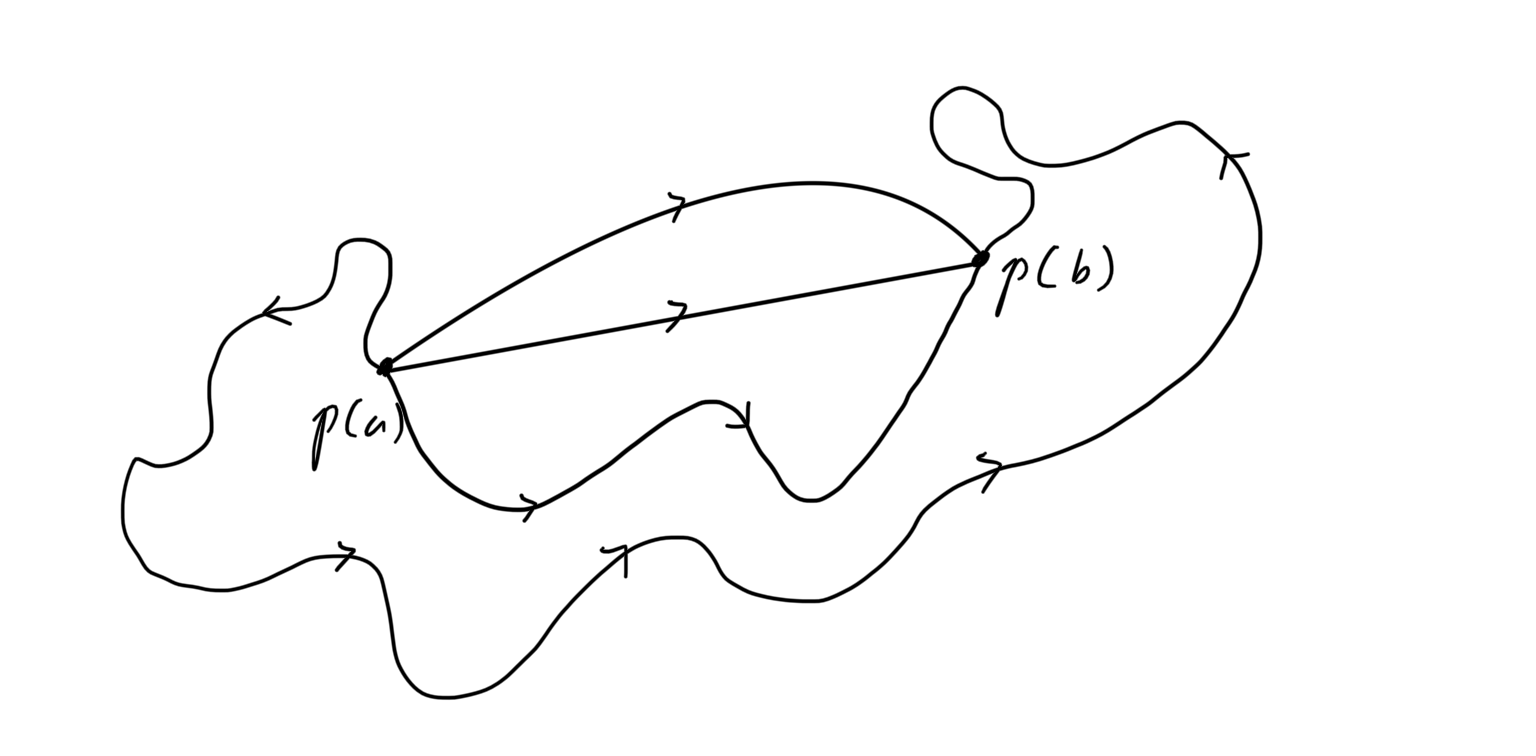
\includegraphics[scale=0.2]{img/Line_Integral_Independence_of_path.PNG}
\end{center}
\end{theorem}

In physics, calculating the work done by a force represented by a vector field requires us to know the path that it travels through. 
\[W = \int_p F \cdot ds\]
However, in many cases $F$ is assumed to be conservative, so it is only necessary that we find the displacement of the particle from its endpoints, resulting in the simplification of the formula.  
\[W = \int_p \nabla f \cdot ds = f\big( p(b)\big) - f \big(p(a)\big)\]

\begin{corollary}[Equivalent Conditions for Vector Field to be Conservative]
The following conditions are equivalent: 
\begin{enumerate}
    \item $F: \mathbb{R}^n \longrightarrow \mathbb{R}^n$ is a conservative vector field. 
    \item The line integral of $F: \mathbb{R}^n \longrightarrow \mathbb{R}^n$ in curve $C$ is path independent; that is, if $C_1$ and $C_2$ are two paramaterizations of $C$, 
    \[\int_{C_1} F \cdot ds = \int_{C_2} F \cdot ds\]
    \item Given that $C$ is a closed loop, the line integral of $F: \mathbb{R}^n \longrightarrow \mathbb{R}^n$ across $C$ is $0$. 
    \[\oint_C F \cdot ds = 0\]
    \item The curl of $F: \mathbb{R}^3 \longrightarrow \mathbb{R}^3$ vanishes
    \[\curl{F} = \nabla \times F = \begin{pmatrix}
    \frac{\partial F}{\partial x} \\\frac{\partial F}{\partial y} \\\frac{\partial F}{\partial z} 
    \end{pmatrix} \times \begin{pmatrix}
    F_1\\F_2\\F_3
    \end{pmatrix}= 0\]
    \item The following partial derivatives of $F: \mathbb{R}^2 \longrightarrow \mathbb{R}^2$ are equal
    \[\frac{\partial F_1}{\partial y} = \frac{\partial F_2}{\partial x}\]
\end{enumerate}
\end{corollary}

We can develop a bit of intuition to determine whether a vector field is conservative or not. If vector field $F$ is conservative, then there exists a smooth scalar field $f$ such that $\nabla f = F$. For each latitude and longitude on a certain map, we can give it an altitude as a function of those coordinates (picture a map with a bunch of hills and valleys). The gradient and thus the vector field is all the vectors that point in the direction of highest ascent. he vector field is all the vectors that point in the direction of highest ascent. Extending the metaphor the path integral is like starting on at a point and climbing the hills and valleys, creating work as you go up a hill (proportional to the steepness and thus the dot product of your motion vector with the gradient vector field in the path integral) and decreasing the work you put in by going down a hill. Since the path is closed, it is like you are going up and down the same amount overall, so the path integral is zero. Following this analogy, the vector field determined by this function (marked as arrows in the $x, y$ plane) is conservative. 
\begin{center}
    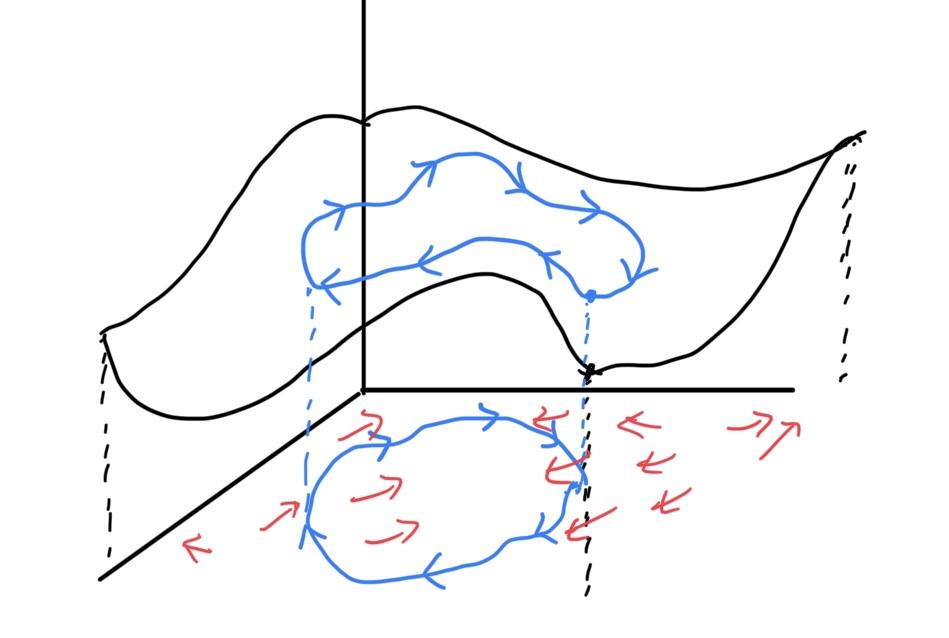
\includegraphics[scale=0.28]{img/Conservative_Vector_Field.jpg}
\end{center}
If we can construct a closed loop around $F$ where the line integral is nonzero, then it means that we have ended up at a "higher" or "lower" (altitude) at the same point. This means that rather than being a certain landscape, there exist different "levels" of values at one point, like a spiraling staircase. For example, look at the solenoidal vector field below, where we can construct a closed loop (a circle going around the origin counterclockwise). There is no "surface" that can be defined such that it contains the solenoid. 
\begin{center}
    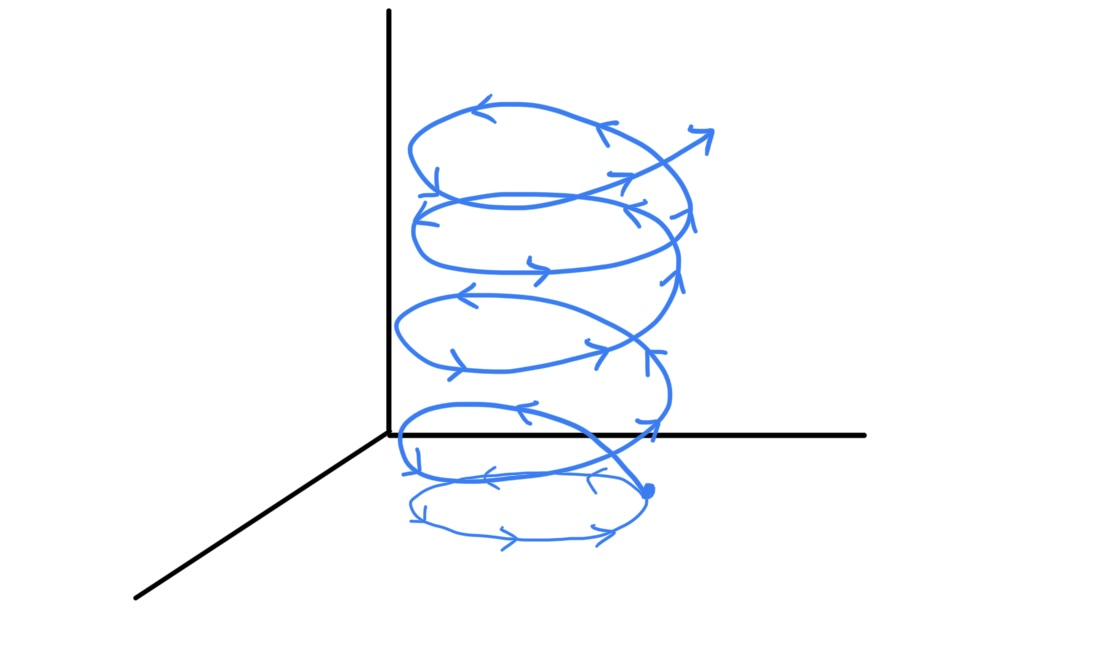
\includegraphics[scale=0.28]{img/Solenoid_nonconservative.jpg}
\end{center}
Clearly, as a particle travels through the vector field along the path, it does positive work while it has zero displacement, and clearly, there exists no function that can output both these values as determined by vector field $F$. 

\begin{theorem}[Helmholtz Decomposition]
Let $F: \mathbb{R}^3 \longrightarrow \mathbb{R}^3$ be a $C^2$ vector field. Then, $F$ can be decomposed into a curl-free component and a divergence-free component. That is, there exists vector fields $A$ and $\Phi$
\[F = - \nabla \cdot \Phi + \nabla \times A\]
\end{theorem}

\subsubsection{Curvature}
\begin{definition}[Curvature at a Point]
Let $c: [a, b] \longrightarrow C \subset \mathbb{R}^3$ be a unit-speed paramaterization of $C$, meaning that $||c^\prime (t)|| = 1$ for all $t \in [a,b]$, and let $p = c(t_0)$ be a point in $C$. The \textit{curvature} $\kappa(p)$ at $p$ is a mapping defined
\[\kappa: C \longrightarrow \mathbb{R}, \;\; \kappa(p) \equiv ||c^{\prime \prime} (t_0)||\]
Notice that since we require a unit speed paramaterization of $C$, we do not need to worry about how a given curve is paramaterized. 
\end{definition}

Since the curvature is defined pointwise for each point in curve $C$, we can integrate over all the curvatures in $C$ to define the total curvature. 

\begin{definition}[Total Curvature]
The \textit{total curvature} of a curve $c: [a,b] \longrightarrow C \subset \mathbb{R}^3$ is the scalar line integral 
\[\int_C \kappa \, ds\]
\end{definition}

We now present an important theorem in differential geometry. 
\begin{theorem}[Fary-Milnor Theorem]
Given a unit speed paramaterization $c: [a,b] \longrightarrow C \subset \mathbb{R}^3$, if $C$ is closed (that is, $c(a)=c(b)$), then 
\[\oint_C \kappa\, ds \geq 2 \pi\]
and equals $2\pi$ only when $C$ is a circle. Furthermore, if $C$ is a closed space curve with 
\[\oint_C \kappa\, ds \leq 4\pi\]
then $C$ is "unknotted." That is, $C$ can be continuously deformed without every intersecting itself into a planar circle. Therefore, for knotted curves $C$, we have
\[\oint_C \kappa \, ds > 4\pi\]
\end{theorem}

\subsection{Surface Integrals}
Surface integrals are the $2$-dimensional analogue, or the double integral version, of line integrals. It is the integration of surfaces. 

\subsubsection{2-Dimensional Paramaterizations of Surfaces}
Just like how we create path functions using a paramaterization function $p: [a, b] \subset \mathbb{R} \longrightarrow \mathbb{R}^n$, we can parameterize surfaces by defining a function 
\[\varphi: D \subset \mathbb{R}^2 \longrightarrow \mathbb{R}^n, \;\;\; \varphi (u, v) \equiv \begin{pmatrix} x_1 (u, v) \\ \vdots \\ x_n (u, v) \end{pmatrix}\]
The surface 
\[S = \varphi(D)\]
corresponding to the function $\varphi$ is its image. If $\varphi$ is differentiable or is of class $C^1$, then we call $S$ a \textit{differentiable} or $C^1$ surface, respectively. 

For those that are familiar with differential geometry, this makes every paramaterized surface a 2-manifold induced by the single homeormophism $\varphi$. In fact, it is more than just locally homeomorphic; it is \textit{globally} homeomorphic. 


\begin{definition}[Tangent Vectors of Surfaces Embedded in $\mathbb{R}^3$]
Given surface paramaterization 
\[\varphi: \mathbb{R}^2 \longrightarrow \mathbb{R}^3, \;\;\; \varphi(u, v) \equiv \begin{pmatrix}
x (u, v) \\ y(u, v) \\ z(u, v) 
\end{pmatrix}\]
it is visually clear that there can be up to two linearly independent tangent vectors at a point on the surface $S$. We can calculate these two vectors by embedding two nonparallel paths in $D \subset \mathbb{R}^2$ and taking the derivative with respect to a point traveling through these paths, which would give us a tangent vector on $S$. To keep things simple, we take the partial derivatives with respect to $u$ and $v$. 
\begin{center}
    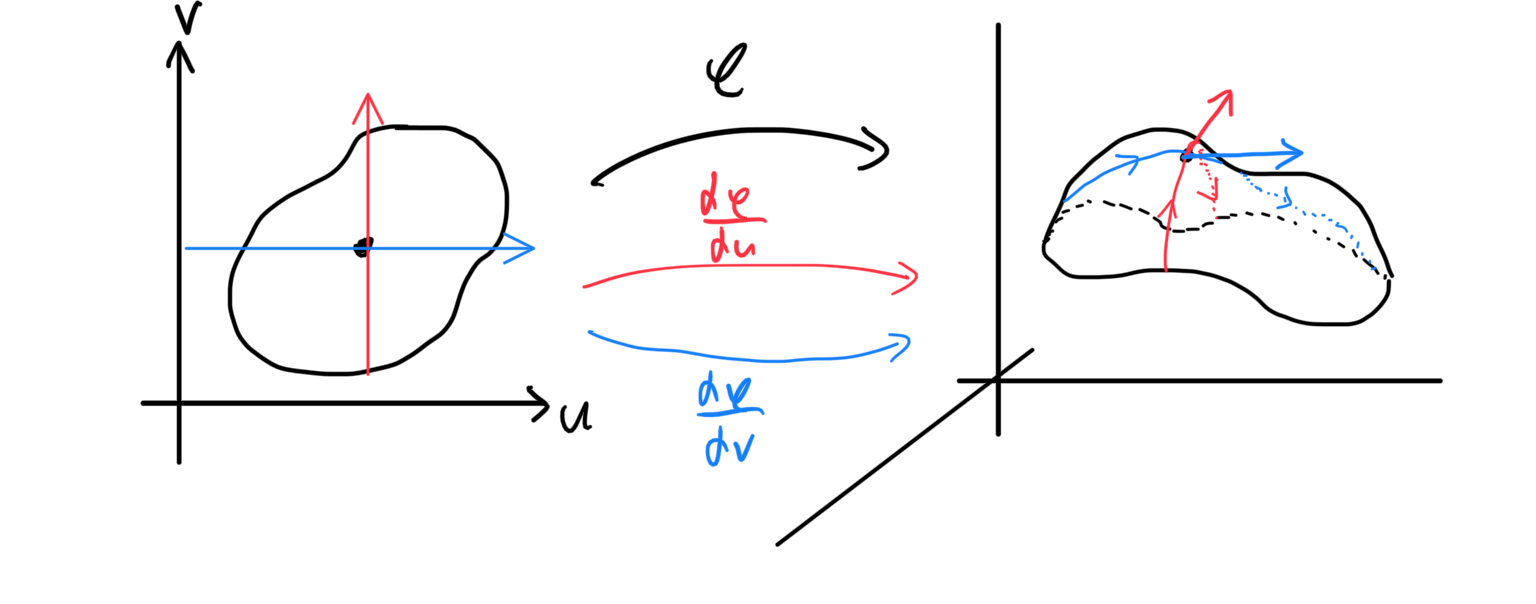
\includegraphics[scale=0.28]{img/Partial_Derivatives_with_respect_to_U_V.PNG}
\end{center}
Clearly, these paths are functions 
\begin{align*}
    \frac{\partial \varphi}{\partial u} \equiv \begin{pmatrix}
     \frac{\partial x}{\partial u} \\ \frac{\partial y}{\partial u} \\ \frac{\partial z}{\partial u}
    \end{pmatrix} : \mathbb{R}^2 \longrightarrow \mathbb{R}^3\\
    \frac{\partial \varphi}{\partial v} \equiv \begin{pmatrix}
     \frac{\partial x}{\partial v} \\ \frac{\partial y}{\partial v} \\ \frac{\partial z}{\partial v}
    \end{pmatrix} : \mathbb{R}^2 \longrightarrow \mathbb{R}^3
\end{align*}
where 
\[\frac{\partial \varphi}{\partial u} (u_0 ,v_0), \; \frac{\partial \varphi}{\partial v} (u_0, v_0)\]
represent two vectors in $\mathbb{R}^3$ that are tangent to $S$ at the point $\varphi(u_0, v_0) \in \mathbb{R}^3$. 
\end{definition}

We must make sure that the surface $S$ is smooth in the sense that (informally) there aren't any wrinkles, points, folds, or self-intersections in such a way that the tangent plane to the surface is not well-defined. 

\begin{definition}[Regular Surfaces]
To formalize this concept, we say that $S$ is \textit{regular}, or \textit{smooth}, at point $(u_0, v_0)$ if
\[\frac{\partial \varphi}{\partial u} \times \frac{\partial \varphi}{\partial v} \neq 0\]
where $\times$ is the Euclidean cross product. That is, if the vector that is orthogonal to the two tangent vectors is well defined at a point, the surface is said to be smooth at that point. Note that $\frac{\partial \varphi}{\partial u}$ is parallel to $\frac{\partial \varphi}{\partial v}$ if and only if their cross product is $0$. 
\begin{center}
    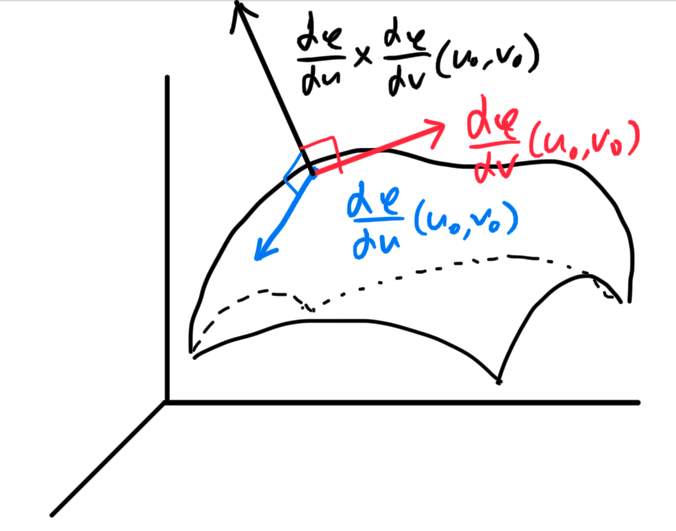
\includegraphics[scale=0.3]{img/Cross_Product_Regular_Surfaces.PNG}
\end{center}
It is quite clear that $(\frac{\partial \varphi}{\partial u} \times \frac{\partial \varphi}{\partial v})(u_0, v_0) \neq 0 \implies \frac{\partial \varphi}{\partial u}$ and $\frac{\partial \varphi}{\partial v}$ are linearly independent. This means that an entire span of tangent vectors, i.e. a tangent plane, of the surface $S$ at $\varphi(u_0, v_0)$ exists. 
$S$ is said to be \textit{regular} if it is regular at all points $\varphi(u_0, v_0) \in S$. 
\end{definition}

In fact, the tangent plane at $\varphi(u_0, v_0)$ is the set of points 
\[\{\varphi(u_0, v_0) + \frac{\partial \varphi}{\partial u} (u_0, v_0) c_1 + \frac{\partial \varphi}{\partial v} (u_0, v_0) c_2 \; | \; c_1, c_2 \in \mathbb{R} \}\]
which is precisely the affine tangent plane spanned by $T_u$ and $T_v$. Note also that the vector $T_u \times T_v$, if nonzero, is normal to this plane, which leads to this equivalent definition. 

\begin{definition}[Tangent Planes of Surfaces]
Given a paramaterized surface $\varphi: D \subset \mathbb{R}^2 \longrightarrow \mathbb{R}^3$ that is regular at $\varphi(u_0, v_0)$, the tangent plane of the surface $S$ at $\varphi(u_0, v_0) = (x_0, y_0, z_0)$ is defined
\[\{(x, y, z) \in \mathbb{R}^3 \;|\; (x-x_0, y-y_0, z-z_0) \cdot n = 0\}\]
where $n = (\frac{\partial \varphi}{\partial u} \times \frac{\partial \varphi}{\partial v})(u_0, v_0)$. 
\end{definition}

We finally construct the concept of signed areas before defining surface integration. 
We have all the tools we need to calculate surface areas, but remember that integration also covers the concept of \textit{signed areas}, which could be negative. In order to define this, we define the concept of orientation on surfaces. 

\subsubsection{Orientation of Surfaces}

\begin{definition}[Oriented Surfaces]
An \textit{oriented surface} is a two-sided surface with one side specified as the \textit{outside/positive} side and the other side as the \textit{inside/negative} side. Note that an oriented surface is not guaranteed to have two sides (e.g. a Mobius strip). To ensure that there exist two sides, $S$ must be regular. 

Surprisingly, a paramaterization does not have an intrinsic orientation. Rather, we determine the orientation ourselves by choosing a unit vector that generally points towards the outside of the surface $S$. Again, this choice is arbitrary, but it is customary to choose a vector that generally points "out." Either way, the orientation (unit) vector at every point $\varphi(u, v) \in S$, denoted as $n$, is 
\[n\big(\varphi(u, v)\big) = \pm \frac{\frac{\partial \varphi}{\partial u} \times \frac{\partial \varphi}{\partial v}}{\big|\big|\frac{\partial \varphi}{\partial u} \times \frac{\partial \varphi}{\partial v}\big|\big|}\]
which can be visually calculated using the right hand rule. 
\begin{center}
    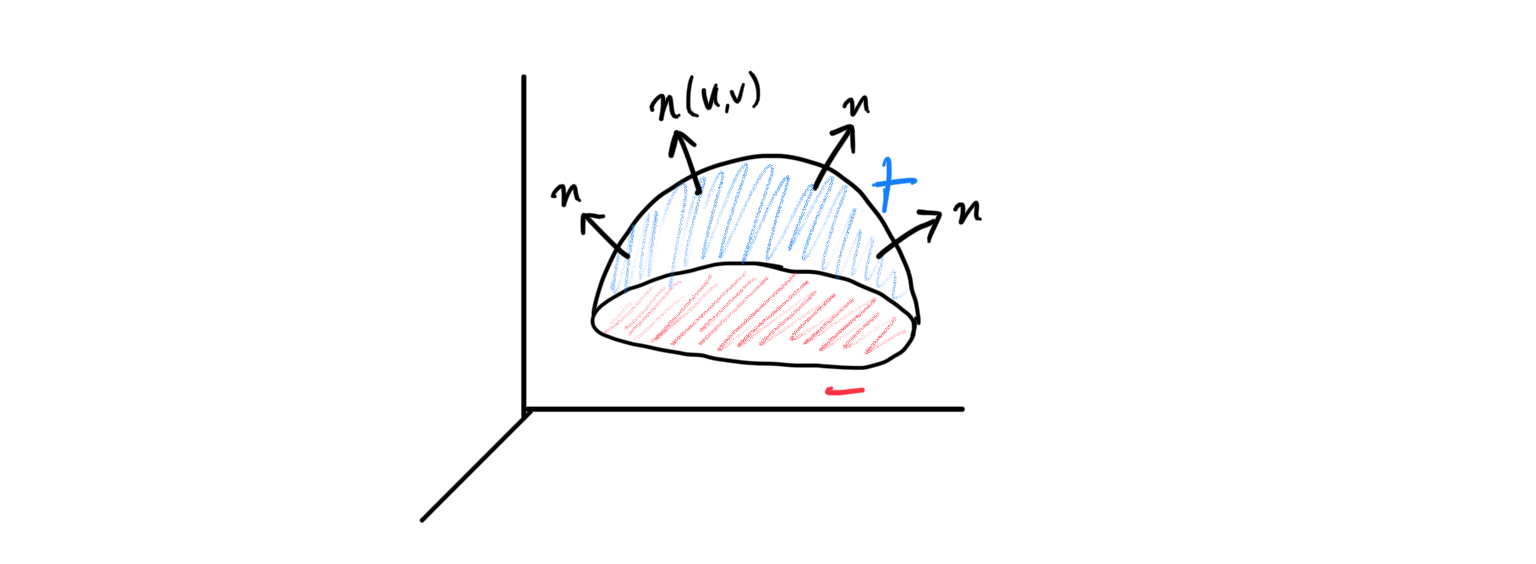
\includegraphics[scale=0.23]{img/Orientation_Unit_Vector.PNG}
\end{center}
\end{definition}

\begin{definition}[Orientation Preserving, Reversing Paramaterizations]
Given an oriented surface $S$ with its positive side determined by the direction of unit vector $n\big( \varphi(u,v)\big)$, the paramaterization $\varphi$ is said to be \textit{orientation preserving} if 
\[n \big( \varphi(u, v)\big) = \frac{\frac{\partial \varphi}{\partial u} \times \frac{\partial \varphi}{\partial v}}{\big|\big|\frac{\partial \varphi}{\partial u} \times \frac{\partial \varphi}{\partial v}\big|\big|}\]
and \textit{orientation reversing} if
\[n \big( \varphi(u, v)\big) = - \frac{\frac{\partial \varphi}{\partial u} \times \frac{\partial \varphi}{\partial v}}{\big|\big|\frac{\partial \varphi}{\partial u} \times \frac{\partial \varphi}{\partial v}\big|\big|}\]
\end{definition}

So, to find whether a paramaterization is orientation preserving or reversing, it suffices to find the cross product $T_u \times T_v$ and see if it points in the same direction of the normal vector $n$ (which should have already been determined when deciding the orientation of $S$). 

Given a paramaterization $\varphi$ and an un-oriented surface $S$, we can also just construct $\varphi$ to be orientation-preserving (or reversing) by \textit{defining} the normal vector $n$ to be 
\[n\big( \varphi(u, v)\big) = \frac{\frac{\partial \varphi}{\partial u} \times \frac{\partial \varphi}{\partial v}}{\big|\big|\frac{\partial \varphi}{\partial u} \times \frac{\partial \varphi}{\partial v}\big|\big|} \;\; \bigg( \text{or } n\big( \varphi(u, v)\big) = - \frac{\frac{\partial \varphi}{\partial u} \times \frac{\partial \varphi}{\partial v}}{\big|\big|\frac{\partial \varphi}{\partial u} \times \frac{\partial \varphi}{\partial v}\big|\big|} \bigg)\]
So rather than finding out whether a paramaterization $\varphi$ is orientation preserving or reversing by comparing $T_u \times T_v$ with $n$, we have defined $n$ in a way such that $\varphi$ must be orientation preserving (or reversing). We can utilize these tools of paramaterization to now define the surface integral. 

\subsubsection{Scalar, Vector Surface Integrals}

A physical interpretation of a scalar surface integral is the weighted surface area of a certain surface. 

\begin{definition}[Scalar Surface Integrals]
Let $f: \mathbb{R}^3 \longrightarrow \mathbb{R}$ be a $C^1$ scalar field defined on a paramaterized surface $S \subset \mathbb{R}^3$ with paramaterization $\varphi: D \subset \mathbb{R}^2 \longrightarrow \mathbb{R}^3$. That is, $\varphi(D) = S$. We define the integral $f$ over $S$ to be
\begin{align*}
    \iint_S f \; dS & = \iint_S f(x, y, z) \; dS \\
    & = \iint_D f\big( \varphi(u, v)\big) \bigg|\bigg|\frac{\partial \varphi}{\partial u} \times \frac{\partial \varphi}{\partial v}\bigg|\bigg| \; du \,dv
\end{align*}
Note that this will require us to transform $f$, a function of $x, y, z$, into the function $f \circ \varphi$ of $u, v$. Additionally, if the paramaterization of the surface $S$ is not defined, then it one must be constructed. It is also clear that if $S$ is a union of surfaces $S_i$, then its surface integral is the sum of the surface integrals of the $S_i$'s. 
\end{definition}

Letting the scalar field $f$ be the constant field equal to $1$, the scalar surface integral measures the surface area of $S$. 
\[A(S) = \iint_S \; dS = \iint_D \Big|\Big|\frac{\partial \varphi}{\partial u} \times \frac{\partial \varphi}{\partial v}\Big|\Big| \; du\, dv\]
It is easy to see that the orientation of the paramaterization $\varphi$ does not affect scalar surface integrals, since the sign of the orientation gets nullified by the absolute value sign over $||\frac{\partial \varphi}{\partial u} \times \frac{\partial \varphi}{\partial v}||$. 

Its physical interpretation is to measure the rate at which a fluid (determined by a vector field $F$) is crossing a given surface $S$. It also has many applications in electromagnetism. 

\begin{definition}[Vector Surface Integrals]
Let $F$ be a vector field defined on surface $S$, the image of a paramaterized surface $\varphi$. The \textit{surface integral} of $F$ over $S$ is defined below, which is equivalent to summing up the dot product of the vector field and the normal vector to the surface. 
\begin{center}
    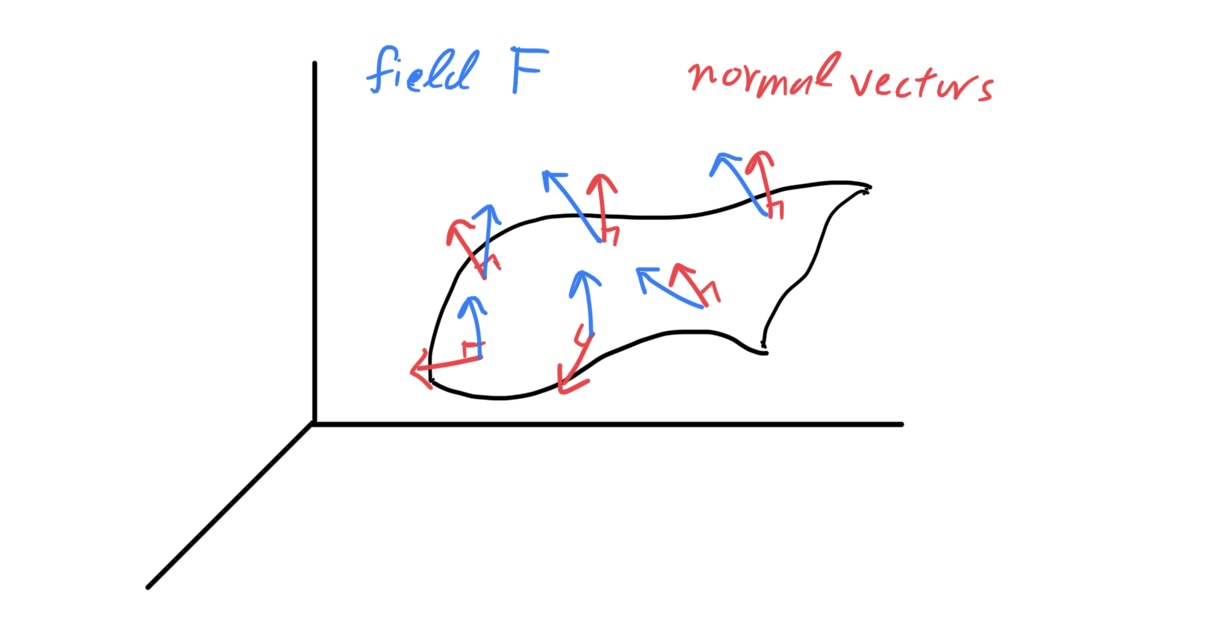
\includegraphics[scale=0.3]{img/Vector_Surface_Integral.jpg}
\end{center}
It can be calculated with the following formulas by converting it into a scalar surface integral where the scalar field is the value of the dot product of the vector field with the normal vectors of the surface. 
\begin{align*}
    \iint_{S} F \cdot d S & = \iint_S (F \cdot n) \; dS \\
    & = \iint_D \Bigg( F\big( \varphi(u, v)\big) \cdot \frac{\frac{\partial \varphi}{\partial u} \times \frac{\partial \varphi}{\partial v}}{\Big|\Big|\frac{\partial \varphi}{\partial u} \times \frac{\partial \varphi}{\partial v} \Big|\Big|} \Bigg) \, \bigg|\bigg|\frac{\partial \varphi}{\partial u} \times \frac{\partial \varphi}{\partial v}\bigg|\bigg|\; du\,dv \\
    & = \iint_D F\big(\varphi(u, v)\big) \cdot \bigg( \frac{\partial \varphi}{\partial u} \times \frac{\partial \varphi}{\partial v}\bigg) \; du\,dv
\end{align*}
\end{definition}

Since we are now talking about vector fields, the orientation of the paramaterization is now significant. Visually, if the orientation of the surface $S$ generally aligns with the vector field $F$, then the integral will be positive (since two vectors $\alpha, \beta$ generally pointing in the same direction implies that $\alpha \cdot \beta > 0$). The orientation of the paramaterization, which is dependent on $\frac{\partial \varphi}{\partial u} \times \frac{\partial \varphi}{\partial v}$, determines the direction of the normal vector $n$ (since it is defined to be $(\frac{\partial \varphi}{\partial u} \times \frac{\partial \varphi}{\partial v}) / \big|\big|\frac{\partial \varphi}{\partial u} \times \frac{\partial \varphi}{\partial v}\big|\big|$. Therefore, changing the orientation of $\varphi$ will reverse the direction of $n$, which will then reverse the sign of the integral since $n$ now points in the opposite direction of the vector field $F$ than it previously did (by reversing the sign of the dot products). This is formalized in the theorem below. 

\begin{theorem}[Invariance of Surface Paramaterizations on Vector Surface Integrals]
Let $S$ be an oriented surface and let $\varphi_1$ and $\varphi_2$ be two regular paramaterizations with $F$ a continuous vector field defined on $S$. Then, assuming $\varphi_1$ is orientation preserving, 
\begin{align*}
    \varphi_2 \text{ is orientation preserving } & \implies \iint_{\varphi_1} F \cdot d S = \iint_{\varphi_2} F \cdot d S \\
    \varphi_2 \text{ is orientation reversing } & \implies - \iint_{\varphi_1} F \cdot d S = \iint_{\varphi_2} F \cdot d S 
\end{align*}
\end{theorem}

\subsubsection{Surface Integrals over Graphs}
Given that we have the graph of a function $g: \mathbb{R}^2 \longrightarrow \mathbb{R}$ rather than a general surface, we can paramaterize it simply as
\[\varphi(u, v) \equiv \big(u, v, g(u, v) \big)\]
\begin{center}
    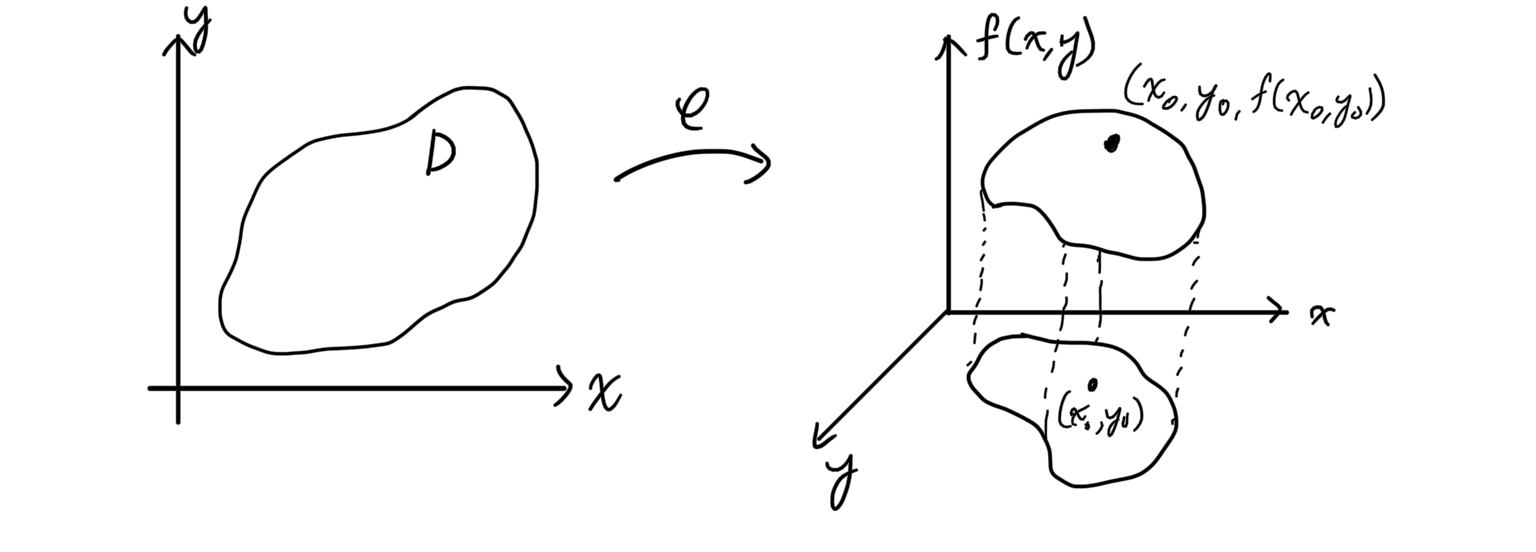
\includegraphics[scale=0.25]{img/Paramaterize_Surfaces_as_Graphs.PNG}
\end{center}
This means that 
\[\frac{\partial \varphi}{\partial u} \times \frac{\partial \varphi}{\partial v} = 
\begin{pmatrix}
-\frac{\partial g}{\partial u} \\ -\frac{\partial g}{\partial v} \\ 1
\end{pmatrix} \implies \bigg|\bigg|\frac{\partial \varphi}{\partial u} \times \frac{\partial \varphi}{\partial v} \bigg|\bigg| = \sqrt{1 + \Big(\frac{\partial g}{\partial u}\Big)^2 + \Big( \frac{\partial g}{\partial v}\Big)^2}\]
So we can simplify the equation for the surface area $S$ of the graph of $g$ over the region $D$ in the $x y$-plane, as 
\begin{align*}
    A(S) & = \iint_S \; d S = \iint_D \bigg|\bigg|\frac{\partial \varphi}{\partial u} \times \frac{\partial \varphi}{\partial v} \bigg|\bigg| \; d A \\
    & = \iint_D \sqrt{1 + \Big(\frac{\partial g}{\partial u}\Big)^2 + \Big( \frac{\partial g}{\partial v}\Big)^2} \; d u \, d v
\end{align*}
With the same $g$, we can find the weighed surface area of $S$ over the scalar function $f: \mathbb{R}^3 \longrightarrow \mathbb{R}$ with the formula
\[\iint_S f \; d S = \iint_D f\big(u, v, g(u, v)\big) \sqrt{1 + \Big(\frac{\partial g}{\partial u}\Big)^2 + \Big( \frac{\partial g}{\partial v}\Big)^2} \; d u \, d v\]
Finally, with the same graph $g$, the surface integral over the vector field $F$ is
\begin{align*}
    \iint_S F \cdot d S & = \iint_D F\big(\varphi(u, v)\big) \cdot \bigg( \frac{\partial \varphi}{\partial u} \times \frac{\partial \varphi}{\partial v}\bigg) \; d u \, d v \\
    & = \iint_D \bigg( F_1(u, v) \Big(- \frac{\partial g}{\partial u}\Big) + F_2 (u, v) \Big( - \frac{\partial g}{\partial v} \Big) + F_3 (u, v) \bigg) \; d u \, d v
\end{align*}

\subsection{Integral Theorems}
Recall the differential notation for writing line integrals. For 2 and 3 dimensions, it is written as
\begin{align*}
    & \int_C F \cdot d s = \int_C F \cdot (d x, d y) = \int_C F_1 \, d x + F_2 \, d y \\
    & \int_C F \cdot d s = \int_C F \cdot (d x, d y, d z) = \int_C F_1 \, d x + F_2 \, d y + F_3 \, d z 
\end{align*}
\subsubsection{Green's Theorem}
Green's Theorem gives the relationship between a line integral around a simple closed curve $C$ and a double integral over the plane region $D$ bounded by $C$. 

\begin{theorem}[Green's Theorem in $\mathbb{R}^2$]
Let there be a 2-dimensional $C^1$ vector field $F$ on $\mathbb{R}^2$ defined on a simple oriented closed piecewise-smooth curve $C$ and its bounded region $D \subset \mathbb{R}^2$ (that is, $C = \partial D$). Let the orientation of the path of $C$ be such that it is traveling \textit{counterclockwise}, i.e. a point traveling through $C$ would see the region $D$ to its \textit{left}, denoted as $C^+$ and the clockwise orientation as $C^-$.  Then, 
\[\oint_{C^+} F_1 \, d x + F_2 \, d y = \iint_D \bigg( \frac{\partial F_2}{\partial x} - \frac{\partial F_1}{\partial y} \bigg) \; d x \, d y\]
By reversing the orientation, it is clear that we have
\[\oint_{C^-} F_1 \, d x + F_2 \, d y = - \iint_D \bigg( \frac{\partial F_2}{\partial x} - \frac{\partial F_1}{\partial y} \bigg) \; d x \, d y\]
Note that this theorem is expressed in terms of the components of the vector field $F$. 
\begin{center}
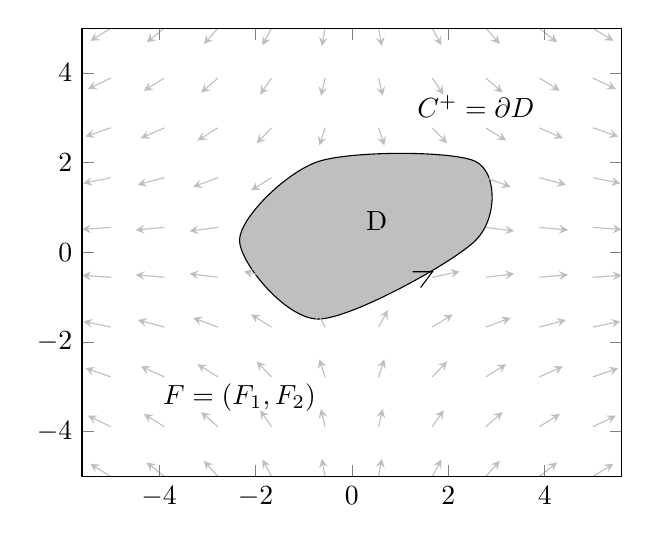
\begin{tikzpicture}
    \draw[fill=lightgray] plot [smooth cycle] coordinates {(2,3) (3,4) (5,4) (5,3) (3,2)};
    \node [above left] at (4,3) {D};
    \begin{axis}[view={0}{90}]
    \addplot3 [lightgray,-stealth,samples=10,
        quiver={
            u={3*x/pow(x^2 + y^2,1/2)},
            v={-2*y/pow(x^2 + y^2,1/2)},
            scale arrows=0.2,
        },] { 1};
    \end{axis}
    \node at (2,1) {$F = (F_1, F_2)$};
    \node at (5,4.7) {$C^+ = \partial D$};
    \draw (4.3,2.4)--(4.45,2.6)--(4.2,2.6);
\end{tikzpicture}
\end{center}
\end{theorem}

Green's theorem has many applications in physics. For example, in order to solve two-dimensional flow integrals measuring the sum of fluid outflowing from a volume, Green's theorem allows us to calculate the total outflow summed about an enclosing area . 

\begin{corollary}
Let $D$ be a region for which Green's theorem applies with positively oriented boundary $\partial D$. Then, the area of $D$ can be computed with the formula
\[A(D) = \frac{1}{2} \oint_{\partial D} x \, d y - y \, d x\]
\end{corollary}

Green's theorem can be used to determine the area of centroid of plane figures solely by integrating over the perimeter. 

\subsubsection{Stokes' Theorem}
Green's theorem relates line integrals to double integrals. Stokes' theorem generalizes Green's theorem by relating line integrals to surface integrals of 2-dimensional surfaces embedded in $\mathbb{R}^3$. 

\begin{theorem}[Stokes' Theorem]
Let $S$ be an oriented regular surface defined by paramaterization $\varphi: D \subset \mathbb{R}^2 \longrightarrow \mathbb{R}^3$, and let the image of the boundary $\partial D$ under $\varphi$ be the boundary $\partial S$ of $S$. We can interpret $\partial S$ as a path mapping from $\mathbb{R} \longrightarrow S \subset \mathbb{R}^3$. 
\begin{center}
  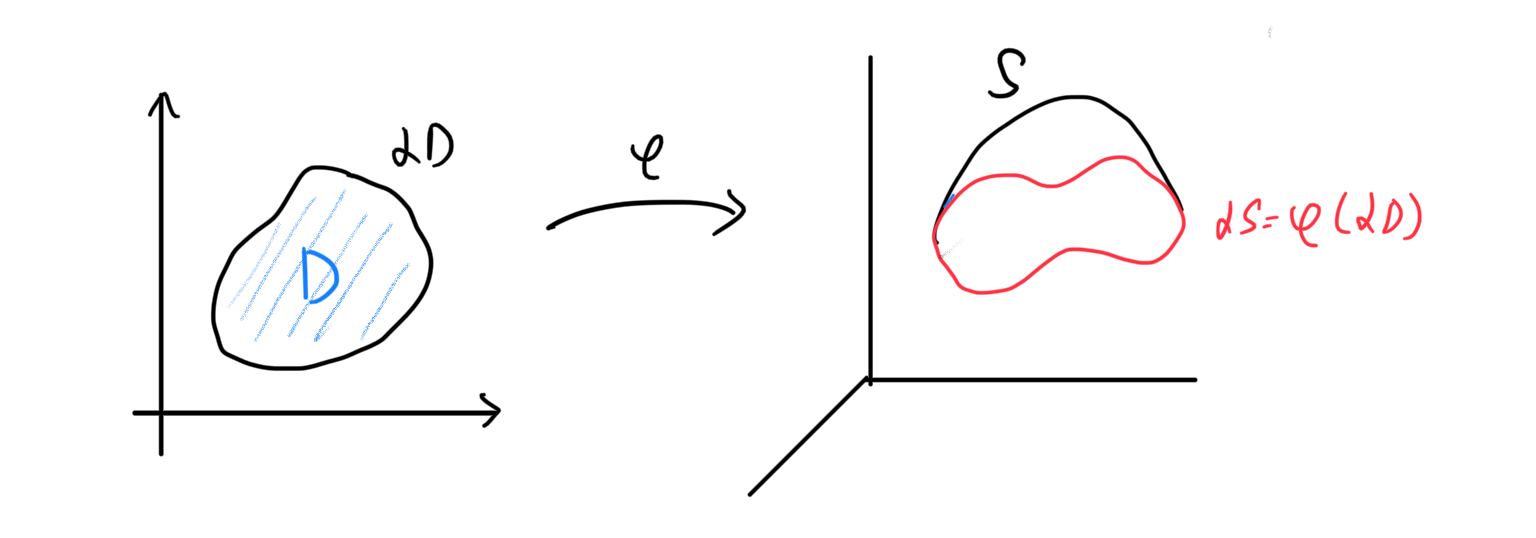
\includegraphics[scale=0.27]{img/Boundary_Mapping.PNG}
\end{center}
The orientation unit vector $n$ of $S$ induces the positive orientation of $\partial S$, denoted $\partial S^+$. Visually, if you are walking along the curve with your head is pointing in the same direction as the unit normal vectors while the surface is on the left then you are walking in the positive direction on $\partial S$. 
\begin{center}
    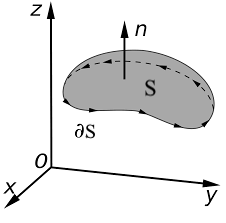
\includegraphics[scale=0.8]{img/Stokes_Theorem_Orientation.png}
\end{center}
Given that $F$ is a $C^1$ vector field defined on $S$, then
\[\iint_S \curl{F} \cdot dS = \iint_S \big( \nabla \times F \big) \cdot d S = \oint_{\partial S^+} F \cdot d s\]
If $S$ has no boundary, that is, if the image of $p^\prime = \partial S$ is not a simple closed curve, then the integral is $0$. 
\end{theorem}

The above theorem implies that the vector surface integral of a surface without a boundary (i.e. a closed graph, such as a sphere) is always $0$ along the curl of any $C^1$ field. Geometrically, this means that given a closed solid $S$ with field $\nabla \times F$, the rate of flow of the vector field into $S$ is equal to the flow out of $S$. 

\subsubsection{Gauss' Theorem}
The divergence theorem relates the flux of a vector field through a closed surface to the divergence of the field in the volume enclosed. 

\begin{theorem}[Gauss' Divergence Theorem]
Let $V$ be a subset of $\mathbb{R}^3$. Denote by $\partial V$ the oriented closed surface that bounds $V$ (with outward pointing normal orientation vectors), and let $F$ be a $C^1$ vector field defined on a neighborhood of $V$. Then, 
\[\iiint_V \Div{F} \; d V = \iiint_V (\nabla \cdot F) \; d V = \oiint_{\partial V} F \cdot d S = \oiint_{\partial V} (F \cdot n) \; dS\]
where the two left-most integrals are volume integrals, and the two right-most integrals are surface integrals. Intuitively, this makes sense; the volume integrals represent the total of the sources in volume $V$, and the right hand side represents the total flow across the boundary $\partial V$. 
\begin{center}
    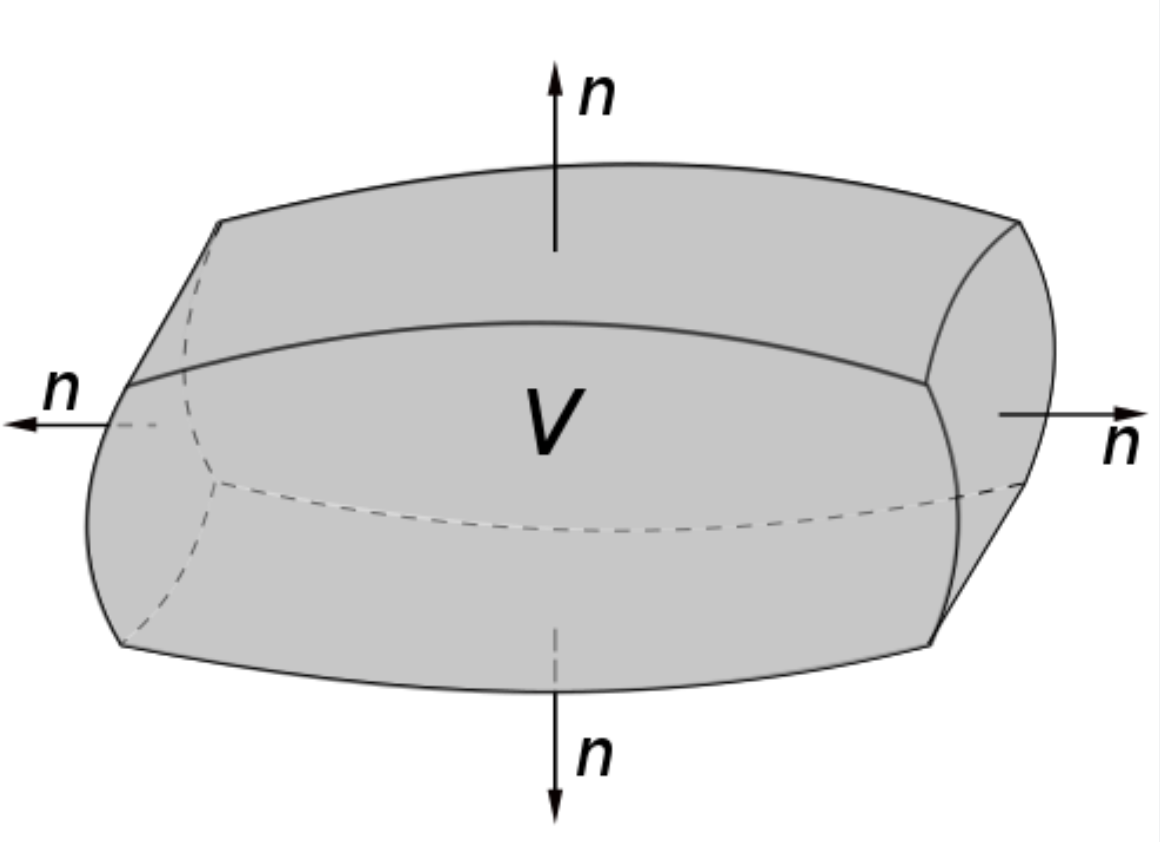
\includegraphics[scale=0.35]{img/Gauss_Theorem_Volume.png}
\end{center}
\end{theorem}



\end{document}

